\documentclass[phdcss]{SDSUThesis}
%\documentclass{article}
\usepackage{amsmath}
\usepackage{amssymb}
\usepackage[utf8]{inputenc}

\usepackage{natbib}
%\usepackage{url}
\usepackage[nottoc,notbib]{tocbibind}

%to get the tilde in \texttt environments
\usepackage[T1]{fontenc}

%I keep getting a fancyhdr warning, this should suppress it
\setlength{\footskip}{4.35004pt}

\renewcommand{\cfttoctitlefont}{\hfill\uppercase}    %TOC Title Font
%\renewcommand{\cfttoctitlefont}{\hfill\bfseries}    %TOC Title Font
%\renewcommand{\cftloftitlefont}{\hfill\bfseries}    %LOF Title Font
\renewcommand{\cftloftitlefont}{\hfill\uppercase}    %LOF Title Font
%\renewcommand{\cftlottitlefont}{\hfill\bfseries}    %LOT Title font
\renewcommand{\cftlottitlefont}{\hfill\uppercase}    %LOT Title font
\renewcommand{\cftaftertoctitle}{\hfill}            %%
\renewcommand{\cftafterloftitle}{\hfill}            %% make titles centered.
\renewcommand{\cftafterlottitle}{\hfill}            %%
\renewcommand{\cftpartfont}{\bfseries}              %Part font
\renewcommand{\cftpartpagefont}{\bfseries}          %Part page# font
\renewcommand{\cftchapfont}{\bfseries}              %Chapter font
\renewcommand{\cftchappagefont}{\bfseries}          %Chapter page# font
% vertical spacing overrides...the default gaps drove me nuts.
\renewcommand{\cftbeforechapskip}{0em}
\renewcommand{\cftbeforepartskip}{0em}
\chapterfont{\centering\nohang\normalsize\bfseries}
\sectionfont{\normalsize\bfseries}


% from https://tex.stackexchange.com/questions/521422/equation-with-numbering-in-table
% for CompFormula table
\usepackage{booktabs}
\usepackage{tabularx}
\usepackage{siunitx}

\usepackage{{makecell}}
\setcellgapes{3pt}\makegapedcells

\usepackage{array,collcell}
\newcommand\AddLabel[1]{%
  \refstepcounter{equation}% increment equation counter
  (\theequation)% print equation number
  \label{#1}% give the equation a \label
}
\newcolumntype{M}{>{\hfil$\displaystyle}X<{$\hfil}} % mathematics column
\newcolumntype{L}{>{\collectcell\AddLabel}r<{\endcollectcell}}


\title{FUNCTIONAL DATA ANALYSIS AND SPATIAL ANALYSIS FOR ON-FARM STRIP TRIALS}
\author{PETER CLAUSSEN}
%\degree{Ph.D.}
%\major{Computational Science and Statistics}
%\docmonth{August}
\docyear{2025}
\docadvisor{Jung-Han Kimn}    % dissertation/thesis advisor name
\depthead{Eun Heui Kim}     % dept head name
\dept{Mathematics \& Statistics}    % department name

%\bibliographystyle{plain}

\usepackage{Sweave}
\begin{document}

\frontmatter

\maketitle

\acceptancepage

\begin{center}
   ACKNOWLEDGMENTS
\end{center}

   Many thanks to Dr. Jung-Han Kimn for his diligent review of this material and his work with the university to help move this work forward, My gratitude to Dr. Chris Saunders for his work; I doubt I'll know all he's done to help me. Much thanks to Dr. Kurt Cogswell who helped put me on the path to this work. Finally, I'd like to thank Kyle Kepner and Margaret Kappenman with GDM Solutions for allowing me the flexibility to pursue my studies.
   


\pagebreak

%\renewcommand{\contentsname}{TABLE OF CONTENTS}
%\begin{center}
%   TABLE OF CONTENTS
%\end{center}

\clearpage
\phantomsection
\pdfbookmark[0]{\contentsname}{contents}
\tableofcontents

%\clearpage

%\listoftables

%\clearpage
%\listoffigures
 
\clearpage

%\begin{center}
%ABSTRACT
%\end{center}

\addcontentsline{toc}{part}{Abstract}
 
 \begin{center}
ABSTRACT
\end{center}

\begin{center}
FUNCTIONAL DATA ANALYSIS AND SPATIAL ANALYSIS FOR ON-FARM STRIP TRIALS
\end{center}

\begin{center}
PETER CLAUSSEN
\end{center}

\begin{center}
2025
\end{center}

Collaborative on-farm trials of agronomic practices have been an established method of interaction between researchers and their target audience (the farmers). With the advent of precision agriculture practices, the on-farm strip trial has become a popular method of collaborative research. Precision agriculture practices allows farmers to precisely control the application of an agronomic product or practice to specific strips in a cropland, and to leave as standard practice strips, or check strips, intermingled with the test strips.

In spite of their popularity, there has been little development in the methods of analyzing strip trials. In this thesis, two examples of strip trials are considered. The first is considered an ideal case of a strip trial, where the test strips are long and narrow and together with the check strips form a uniform rectangle. With this example, methods of analyzing strips as functional data objects are developed and functional paired $t$-tests and functional trend analysis is applied. 

The second example is a strip trial where the test product was applied more haphazardly and performs poorly when the strips are analyzed as functional data. To provide an analysis of these data, the trend analysis is extended to a two-dimensional spatial analysis as a method to determine the effect of the applied product.


\mainmatter

%\clearpage


\clearpage
\phantomsection 
%\addcontentsline{toc}{part}{Chapters}

%\end{abstract}

\Sconcordance{concordance:Thesis.tex:/Users/dakotajudo/Work/git/YieldDataModels/Thesis.Rnw:1 64 1 1 0 49 1 1 5 1 21 6 1 1 %
16 1 1 1 25 163 1 1 14 1 2 14 1 1 14 1 2 10 1 1 4 1 2 3 1 1 12 1 2 169 1 1 5 1 2 8 1 1 5 1 1 1 6 1 2 63 1 1 %
11 1 2 7 1 1 22 1 2 36 1 1 30 15 0 1 2 137 1 1 23 1 1 1 38 1 2 4 1 1 40 1 2 5 1 1 41 1 2 7 1 1 8 1 2 97 1 1 %
28 2 1 1 6 1 2 30 1 1 47 1 1 1 6 1 2 8 1 1 56 1 1 1 7 1 2 7 1 1 64 1 12 1 20 1 25 1 22 1 1 3 21 1 29 1 15 1 %
24 56 1 1 4 1 2 4 1 1 7 1 2 3 1 1 7 1 2 3 1 1 7 1 2 3 1 1 7 1 2 3 1 1 8 1 2 3 1 1 8 1 2 3 1 1 7 1 2 3 1 1 7 %
1 2 4 1 1 7 1 2 33 1 1 6 1 2 21 1 1 51 1 1 1 4 1 2 2 1 1 5 29 1 1 3 14 0 1 2 1 1 1 7 1 2 3 1 1 4 1 2 8 1 1 %
28 1 14 1 1 1 6 1 2 10 1 1 36 1 1 1 6 1 2 8 1 1 33 1 1 1 6 1 2 12 1 1 17 38 1 1 5 1 2 3 1 1 13 27 1 1 5 1 2 %
19 1 1 13 3 1 1 7 1 2 3 1 1 9 1 1 1 4 1 2 12 1 1 7 1 2 4 1 1 7 1 2 4 1 1 7 1 2 13 1 1 24 1 1 1 6 1 2 26 1 1 %
5 1 2 4 1 1 5 1 2 4 1 1 5 1 2 4 1 1 5 1 2 6 1 1 15 1 2 14 1 1 4 25 1 1 6 1 2 3 1 1 40 1 1 1 5 1 2 8 1 1 5 1 %
1 1 6 1 2 3 1 1 38 24 1 1 5 1 2 4 1 1 5 1 2 4 1 1 5 1 2 4 1 1 5 1 2 4 1 1 5 1 2 61 1 1 7 20 1 1 5 5 1 1 5 1 %
2 4 1 1 6 1 2 8 1 1 10 4 1 1 22 1 1 1 5 1 2 4 1 1 5 1 2 3 1 1 5 1 2 30 1 1 6 1 2 7 1 1 8 1 2 6 1 1 5 1 2 13 %
1 1 5 1 2 6 1 1 12 1 27 1 1 1 5 1 2 7 1 1 11 2 1 1 12 1 2 10 1 1 12 1 2 9 1 1 24 1 1 1 5 1 2 3 1 1 21 1 1 1 %
5 1 2 4 1 1 5 1 2 33 1 1 19 1 1 1 5 1 2 9 1 1 20 1 1 1 5 1 2 4 1 1 5 1 2 4 1 1 5 1 2 29 1 1 8 1 30 1 4 1 1 1 %
8 1 2 155 1 1 14 1 2 14 1 1 14 1 2 14 1 1 24 1 1 1 14 1 2 28 1 2 21 1 57 1 101 1 1 1 6 1 2 3 1 1 6 1 2 7 1 1 %
47 1 46 2 1 1 11 1 6 1 1 1 12 1 2 6 1 1 12 1 2 6 1 1 6 1 2 3 1 1 6 1 3 7 1 1 31 1 1 1 7 1 2 4 1 1 7 1 2 12 1 %
1 16 1 20 1 56 108 1 1 7 6 1 1 47 47 1 1 12 1 2 19 1 1 6 1 2 5 1 1 11 24 1 1 20 1 1 1 7 1 2 14 1 1 12 1 16 1 %
60 1 1 1 8 3 1 1 47 1 1 1 6 1 2 3 1 1 16 1 1 1 7 1 2 3 1 1 26 7 1 1 6 1 1 1 14 1 2 4 1 1 16 1 20 1 55 109 1 %
1 5 1 2 3 1 1 47 58 1 1 6 1 3 3 1 1 11 7 1 1 12 1 2 19 1 1 20 1 1 1 7 1 2 56 1 1 11 25 1}


%This document draws from
%FunctionalForms.Rmd
%FunctionalAnalysisStripTrials.Rmd
%FunctionalAnalysisRegression.Rmd
%Spatial Analysis of a Strip Trial
%Spatial Analysis of a Strip Trial Trimmed



%Begin FunctionalAnalysisStripTrials 


%% See ASA_CSSA_SSSA/2018/ThoughtsAboutPower -->

% Data used for this thesis

% Read and process data for example 2

\chapter{Overview}\label{ChapOverview}

Consider the problem of on-farm participatory research. On farm trials have a long history, and one popular model is to provide a farmer-collaborator with a small amount of product (for example, fungicide) to test on a portion of crop lands. The work presented in this thesis works toward a simple goal - can it be determined with some degree of statistical rigor if the product application was effective? The area of design and analysis of on-farm participatory research has not undergone the degree of development, with respect to experimental design and analysis, as the more traditional \textit{small-plot} trials, which have been conducted worldwide in some form for more than a century. The material in this thesis is presented as a contribution toward the development of methods for analysis on-farm strip trials.

\section{Chapter Outline}

Chapter \ref{ChapOnFarmStripTrials} is a review of the literature of on-farm strip trial analysis and discuss the nature of yield monitor data, followed by Chapter \ref{RepresentativeStripTrialsChapter} describing two representative strip trials that will serve as sources for example data analyzed in this thesis. This chapter introduces data before completing the relevant literature review so that examples of functional data from representative trials can be used to motivate later chapters.

Chapter \ref{SmoothingFunctionsChapter} considers how temporal data collected during harvest (harvest passes) can be modeled using spline bases functions. Chapter \ref{UnivariateAndFunctionalDataAnalysisChapter} describes the similarity to traditional \textit{univariate} data analysis to pointwise functional data analysis.

Chapter \ref{FunctionalDataAnalysisChapter} demonstrates the application of pointwise functional data analysis (paired sample $t$-tests) using the smoothed harvest passes as observational units. Chapter \ref{TrendAnalysisChapter} complements Chapter \ref{FunctionalDataAnalysisChapter} by applying a pointwise trend analysis in place of pointwise $t$-tests. Chapter \ref{SpatialAnalysisChapter} extends the pointwise trend analysis over smoothed yield monitor curves in Chapter \ref{TrendAnalysisChapter} to a two dimensional response surface analysis of strip trials, where smoothing criteria is based on the properties of spatial random fields. Finally, Chapter \ref{ConclusionsChapter} presents a summary of the analysis methods presented in this thesis.

It should be noted that this document is example of literate programming. That is, this document contains narrative text with embeded R code using the SWeave syntax \cite{leisch-12-2002}.

\clearpage

\chapter{On-farm strip trials}\label{ChapOnFarmStripTrials}

\section{Overview of on-farm trials}

Collaborative research between agronomists and farmers has a long history \cite{doerge-07-1999, kyveryga-11-2019, riley-03-2001}. The importance of farm-scale experiments was recognized early in the development of the development of agricultural testing \cite{student-12-1923, student-02-1938}. In the internet era, collaboration with, and dissemination of information to farmers has greatly increased. For example, the Nebraska On-Farm Research Network \cite{agriculture-2024} allows users to browse on-farm trials dating to 1990.  Precision agriculture (PA) technologies have greatly increased opportunities for on-farm research (for example, \cite{lawes.r-03-2012, taylor-08-2011}). 


Collaborative trials that are largely conducted by the farmer, independent of researcher intervention are of particular interest. In such cases, farmers are given a sample of a new technology - crop varieties, pesticides, etc - and encouraged to apply the new technology to a small portion of their acreage to demonstrate the effectiveness of the new technology. The farmer benefits by being able to see for himself the effectiveness (or lack thereof) of the new technology, while the researcher benefits from being able to pool the results from multiple collaborators. 


In this thesis, I propose methods specifically to analyze single on-farm strip trials \cite{network-2023, hicks-1997, kyveryga-06-2018}. A strip trial is executed by applying experimental treats to strips that typically span the entire length of a crop land, and in some cases may be arranged to complement traditional small-plot trials. On-farm strip trials can have an advantage over more traditional small plot trials with respect to statistical power in detecting differences among certain kinds of treatments \cite{kandel-2018, li-09-2022, laurent-2022}, typically because the size of the strips are less sensitive to spatial variability inherent in most crop lands. My ultimate goal is to provide a presentation of the results of a strip trial to collaborators that can provide some statistical support to answer the question 
\begin{quotation}
   Did the new product work well enough in the strip trial for the collaborator to adopt the new technology for application to a larger percent of his total acreage?
\end{quotation}

For this thesis, I will define on-farm research as comparative experiments such that

\begin{enumerate}
 \item trials are conducted on farmer-managed crop-lands
 \item treatments are applied using farmer-owned equipment  
 \item data is collected using farmer-owned harvesters 
\end{enumerate}

The term term crop-land will used the for an area of ground planted and harvested by a farmer. The term \textit{field} is more commonly used. There exist mathematical entities known as \textit{random fields}, and the term  \textit{field} will be used to imply the latter context, and \textit{crop-land} for the former.

Further, items 2) and 3) imply the use of GPS-enabled technology to record placement of experimental treatments and the corresponding crop yields, 2) determines the size of the experimental unit, while 3) determines the size of the observational unit. Specifically, the dimensions of the experimental units will be determined by the width of farm implements used to apply treatment and by the length of a typical application pass. In many cases, the width of the application implement is greater than the width of the harvester, so there may be multiple harvest passes per application pass. 

Consider a \textit{pass} as a simple complete farming operation, e.g. the interval between when a planter is lowered into the soil at one end of the field to when the planter is raised at the other end of the field, when a sprayer starts spraying at one of the field and continues to the opposite end of the field, or when a harvester enters unharvested crop at one end of the field and continues in a roughly linear motion to the opposite end. Because of differences in planter or sprayer and harvester widths, there may be multiple harvester passes per planter or sprayer pass. However, experimental products are usually applied at planting time, or at some interval during the growth season, so the basic experimental unit, the \textit{strip} consists of a single pass of a planter or sprayer. Thus, in the analysis of strip trials, I will make the distinction between harvest passes and experimental strips.

In practice, before analysis a pass may be trimmed to exclude the end-of-row headlands, which may include overlapping applications \cite{bullock-11-2019}. Strips should also ideally be applied to inner rows only to avoid side of field effects \cite{bullock-11-2019}. There is inherent spatial variability in the accuracy of yield monitors \cite{gauci-12-2023} and that yield monitor data frequently contains artifacts \cite{marchant-2019} but an appropriate choice of interpolation of yield points can minimize point-to-point variability.


Each strip may be thought of in terms of a traditional plot, albeit a very long and very thin plot, and in some cases the results of a strip trial is presented in a manner analogous to traditional small-plot trials \cite{kandel-2018, laurent-2022}. This practice has a long history \cite{wishart-1934}. However, a strip in the shape a very long and very thin rectangle becomes increasingly similar to a single line, and  yield as function of position on this line can easily be modeled. Thus, the analysis of yield monitor data from strip trials is a likely candidate for functional data analysis, and much of this thesis will be devoted to the representation of strips as functional data, and developing functional data analysis of the strips.


Strictly speaking, on-farm strip trials do no necessarily require the use of GPS enabled harvesters. In the past, weigh wagons have been used to measure yield of strips in on-farm participatory testing, \cite{nelson-06-2015, wuest-1994, yan-03-2002}, for example. However, this method to determine strip yield is not suitable to analysis as functional data; while such methods have been in common use and are valid in context, I will ignore such experiments for my proposed analysis. 

Some on-farm experiment can be conducted as single strips; the methods discussed in this thesis assumes multiple strips. Other methods have been proposed for the analysis of single-strip trials \cite{hatfield-06-2018, cho-2021}. On-farm strip trials may be unreplicated within a single location \cite{yan-03-2002, plant-2007, schmidt-04-2018}. In some cases inferences can be made if the experiment is replicated analyzed across multiple locations \cite{schmidt-04-2018, yan-03-2002}. Methods have proposed that can be used to generate $p$-values of a sort, taking advantage of geospatial correlation within portions of the field \cite{plant-2007, willers-01-2008} These analysis should not be used to make inferences about the difference between treated and untreated analysis protions of a field, primarily because the proposed analyses are based on unreplicated experimental units. On-farm trials may be paired with research station-based traditional small-plot experiments, as with mother-baby trials \cite{snapp-01-1999, virk-2008}.

Bramley, et. al \cite{bramley-10-2022}, discuss on-farm experimentation in the context of checkerboard pattern arrangements. They discuss pros and cons of rigorous statistical analysis of on-farm experiments, but in general are sympathetic to the interpretability of experimental results, particularly in the context of farmer-collaborator observations of the experimental treatments. As their title suggests, they emphasize the \textit{farmer-centric} approach to on-farm experiments, and the software used to present and analyze research results. Following their suggestions, in this thesis soe consideration will be given to the automation of identifying functional forms for strip trial data. Tanaka, et. al, \cite{tanaka-05-2023} describe what might also be called a checkerboard pattern, but buffer space is included between the individual experimental units, unlike \cite{bramley-10-2022}. Tanaka, et. al, describe a fertilizer trial where response is analysed using regression models. While not in strips, thus not compatible with the functional data analysis methods described Chapters \ref{FunctionalDataAnalysisChapter} and \ref{TrendAnalysisChapter}, arrangements of this sort may be amenable to the spatial analysis described in Chapter \ref{SpatialAnalysisChapter}.

\clearpage

\section{Overview of yield monitor data}\label{YieldMonitorOverview}

Yield is recorded in units of bushels per acre. This requires the use of several sensors in the harvester \cite{grisso-2009, whelan-2013, luck-2014}. Grain flow sensors measure the rate at which grain moves within the harvester. Typically, there are two types of sensors in used; impact-type which measures the force of grain hitting a metal plate connected to a strain gauge or potentiometer, and volumetric-type sensors which measure the volume of grain as it is lifted inside the harvester in an elevator. Flow rate is typically recorded at one second intervals as in these example data.

Yield in bushels per acre is usually standardized to a specific grain moisture content, so to properly record yield, harvesters are equipped with grain moisture sensors. There are many types of moisture sensors, but in general, grain moisture is not sampled at the same rate as grain flow; in these example data, moisture measurements are taken at 10-15 second intervals. Moisture is typically reported as a percent water. Yield flow rate volumes are recorded as \textit{wet} weight, and yield monitor software uses to covert grain flow to a standardized \textit{dry} weight.

Harvesters are equipped with ground speed sensors, which measure the speed of the harvester as it travels through the standing crops. This, combined with swath width or cut width (meters or feet, depending on the specific yield monitor), is used by yield monitor software to convert grain flow in weight per second to weight per area, resulting in a dry yield volume. Yield is converted according to the following formula  \cite{luck-2014} :
\begin{equation}
Yield \left( \frac{bushels}{acre} \right) = 43560 \left( \frac{m \times t}{d \times w \times p} \right) \left( \frac{100-MC_{harvest}}{100-MC_{market}} \right)
\end{equation}
where
\begin{itemize}
\item $m$ = mass flow rate ($lb/sec$)
\item $t$ = logging interval of the yield monitoring system ($sec$)
\item $d$ = distance traveled between logged data points ($ft$)
\item $w$ = header cut width setting ($ft$)
\item $p$ = grain density or test weight ($lb/bu$)
\item $MC_{harvest}$ = moisture content from yield monitor sensor (wet weight) ($\%$)
\item $MC_{market}$ = marketable moisture content (dry weight) ($\%$)
\item $43560$ = conversion from $ft^2$ to acres.
\end{itemize}

Yield is mapped to specific geographic coordinates through GPS sensors, which associated a longitude and latitude with each recorded grain flow data point. While each yeild measurement is mapped to a point location, it should be remembered that each point represents an estimate of yield over an area as described above. 

There is a lag between the time the grain enters the combine and when the grain reaches the grain flow sensor; it is usually possible for operators to adjust lag time to improve the accuracy of GPS coordinates associated with yield points. Functional data analysis may be used to align \cite{bivand.r-2013} individual passes to account for this lag, but the alignment of functional data is outside the scope of this thesis.

\clearpage

\section{A survey of methods to analyze on-farm trials}

Piepho, et al, \cite{piepho-11-2011} proposes a method of analysis of strip trials, according to the following algorithm:
\begin{enumerate}
  \item overall assessment of the treatments based on plot-averages
  \item overall assessment of the treatments based on subsamples without taking geo-referencing into account
  \item inspection of residuals from step (2) for associations with covariates
  \item overall assessment of the treatments based on spatial modelling of geo-reference subsamples with and without taking covariates into account
  \item spatial analysis of all geo-referenced subsamples based on categorized deflect angles with and without taking covariates into account.
\end{enumerate}

This method involves dividing the field into 30m grid, with each grid designated as a plot This method does not consider strips as experimental entities, instead the data were averaged and centered on the midpoint each grid, then geospatial methods were applied. This method does have the advantage of incorporation of geospatial information such as EC. Overlaying grids has been a historically recommended method for summarizing yield monitor data \cite{franzen-12-2008}.

\cite{lawes.r-03-2012} produces graphic displays similar to those presented in this thesis. However, instead of finding functional forms for the data, the data were divided into a regular 5 meter grid of $n$ rows by $m$ columns, and pairwise $t$ tests was performed between two rows by subsetting the original $n \times m$ array into groups of five consecutive columns and two rows. The process was repeated by moving the position where the five columns were selected, for a total of $m-5$ total $t$-tests. This method was considered analogous to a moving window regression, with the exception that the windows were used for $t$-tests. This method seems fundamentally flawed since the five columns used a replicates are not independent experimental units \cite{crawford-1997}; as described, the analysis method used with only two rows.

The Iowa Soybean Association On-Farm Research Network provides simple $t$-test based analysis of on-farm trials, but also provides a online, interactive tool (ISOFAST)\cite{laurent-11-2019} for summarizing results of multiple on-farm trials. They generally ignore spatial effects at the field level, but with ISOFAST allow broader geographical tests of the on-farm effectiveness of a variety of agricultural products and practices.


Evans et al. \cite{evans-11-2020} used geographically weighted regression for the analysis of strip trials. This method has the advantage of partitioning variance in strip trials into a spatial variability component and a treatment component. Stefanova, et al. \cite{stefanova-04-2023} used a clustering method to delineate strips into comparable pseudo-environments, then analyzed the resulting clusters as multi-environment trials using linear mixed models. As with ISOFAST, these methods sacrifice local spatial analysis for the good of a broader geographical spatial analysis.

On-farm participatory trials are not limited to strip trials. The Data‐Intensive Farm Management Project (DIFM) \cite{bullock-11-2019} combines randomized blocks of systematically randomized variable rates of inputs in grids. Spatial analysis of strip-plot and split-field trials has also been used with some success \cite{griffin-08-2008}. 


The examples used to present a method of functional analysis are better understood as systematic strip arrangements, as opposed to more traditionally randomized trials. Randomization is key if causal effects are to be investigated, but randomization may not always be practical, so in many cases farmers are recommended to use systematic strips. The relative merits of systematic arrangements versus randomized arrangements has been debated for much longer than strip trials have been made avaiable to farmers \cite{yates-01-1939}. If trends are accounted for, systematic trials can be effective \cite{alesso-11-2019, cao-06-2022}. In the chapter \ref{TrendAnalysisChapter}, trend analysis is incorporated with functional data analysis of a systematic trial.

\clearpage

\chapter{Representative strip trials}\label{RepresentativeStripTrialsChapter}

\section{Overview}

I will be using two distinctly differ data sets as representative of on-farm strip trials. The first example (Example 1) was executed as a uniform rectangle with uniformly-sized experimental units and a relatively uniform crop stand throughout. This represents a best-case scenario for an on-farm trial. 

The second example (Example 2) was executed in a cropland that was not a simple rectangle, such that experimental units are not of the same length. This example represents a case with extensive naturally occuring yield variability \cite{grisso-04-2009} that complicate interpretation of yield maps. This cropland also had areas that were not planted, making this experiment something of a worse-case scenario for obtaining meaningful results that can be communicated to the farmer-collaborator. 

\section{Data conversion from GPS formatted files to R compatible format}

The two example trials trials were conducted independently by different farmer-collaborators, using different harvest equipment. Different yield monitor manufacturers use different native file formats for GPS-tagged yield data. Ag Leader SMS software \cite{agleader} was used to convert the native data from Example 1 to GIS shapefile format \cite{listed-07-1998}; the yield data for Example 2 was exported to GIS shapefile format from John Deere Operations Center (\texttt{operationscenter.deere.com}). 

Shapefiles were read into QGIS \cite{qgis} then exported to CSV format to be imported into R \cite{rcore}. Unless otherwise stated, all data manipulation and statistical analysis were performed using R. Before statistical analysis, the data were anonymized by converting GPS coordinates, which can be used to identify the specific collaborators field, to distance in meters from an origin point. The origin was found by subtracting the minimum latitude or longitude in corresponding data columns from each of the coordinates associated with a yield data point. 

GPS distance units were converted to meters based on the haversine formula \cite{robusto-01-1957} where degrees of latitude or longitude are converted to metric unit by first establishing a midpoint latitude ($lat_{mid}$)for the data to be converted, then calculating meters per degree (of latitude or longitude) according to
\begin{equation}
   \begin{aligned}
      m/deg_{lat} & = 111132.954 - 559.822 * cos( 2.0 * lat_{mid} ) + 1.175 * cos( 4.0 * lat_{mid}) \\
      m/deg_{lon} &= (\pi/180 ) * 6367449 * cos ( lat_{mid} )
   \end{aligned}
\end{equation}
Geotagged yield points in GPS units for latitude and longitude where then multiplied by the appropriate conversion factor to compute geographical tags denoted \texttt{Northing} and \texttt{Easting}. The conversion was computed using an R function adapted from code obtained from \texttt{https://stackoverflow.com/questions/639695/how-to-convert-latitude-or-longitude-to-meters}

%<<add.metric.function, eval = FALSE>>=
%add.metric <- function(data, origin=c(NA,NA)) {
%  #adapted from https://stackoverflow.com/questions/639695/how-to-convert-latitude-or-longitude-to-meters
%  if(any(is.na(origin))) {
%    origin[1] <- min(data[,'X'])
%    origin[2] <- min(data[,'Y'])
%  }
%  data[,'Easting'] <- data[,'X'] - origin[1]
%  data[,'Northing'] <- data[,'Y'] - origin[2]
%  latMid <- (min(data[,'Y']) + max(data[,'Y']))/2
%  m_per_deg_lat = 111132.954 - 559.822 * cos( 2.0 * latMid ) + 1.175 * cos( 4.0 * latMid)
%  m_per_deg_lon = (3.14159265359/180 ) * 6367449 * cos ( latMid )
%  data[,'Easting'] <- data[,'Easting']*m_per_deg_lon
%  data[,'Northing'] <- data[,'Northing']*m_per_deg_lat
%  return(data)
%}
%@

The final version of the data include three columns that are of interest for the proposed analysis:
\texttt{Easting} as the number of meters from the lower left (southwest) corner in an easterly direction of the cropland where the grain was harvested, \texttt{Northing} as the number of meters in a northerly direction, and \texttt{Yield}, which is yield in bushels per acre, renamed from the original data; this was done to make analysis consistent across yield data providers.

\clearpage

\section{Strip trial, Example 1}\label{Example1Section}

\begin{figure}\centering
\includegraphics{Thesis-Example1Maps}
\caption{Seeding and yield monitor harvest maps for Example 1. The upper graph shows that varieties are planing in alternating strips with two harvest passes per strip. The lower graph shows instantaneous yield estimates colored by yield value. There are conspicuous low yielding regions at about 100 m and about 200 m \texttt{Easting}}\label{Example1Maps}
\end{figure}

In this first example, two varieties were tested using a split-planter comparison method \cite{doerge-07-1999}.
Two varieties were assigned to the left and to they right half of a standard corn planter. Variety names were entered in the original data as \texttt{Product}, these were anonymized to letters \texttt{B} and \texttt{E} - this was part of a larger strip trial with additional test varieties.

Grain was harvested  with a GSP enabled combined, with the width of the harvester one-half the planter width. Twelve passes  were planted, representing two planted strips, and 24 passes were harvested. The data were trimmed to excluded head rows and side rows to improve uniformity of the strips. The length of each harvest pass was approximately 400m. The harvest and yield maps are shown in Figure \ref{Example1Maps}. The data were not screened from outliers, after the endrows and edgerows were removed from the analysis there were no meaningful outliers in the remaining data points (Figure \ref{Example1Histogram}).

\clearpage

\section{Strip trial, Example 2}\label{Example2Section}



\begin{figure}\centering
\includegraphics{Thesis-Example2SprayYieldMaps}
\caption{Spraying and yield monitor harvest maps for Example 2. In this example, the boom used to spray the field covered 4 harvest passes, so there are 4 harvest passes per experimental strip. There were also several wetlands that prevented planting in some regions of the cropland.}\label{Example2SprayYieldMaps}
\end{figure}

Example 2 is a fungicide trial where the collaborator was instructed to spray a fungicidal treatment in alternating strips in a field of his choosing; the number and location of strips was also chosen by the farmer. In this case, the collaborator started spraying at the gate leading into the field and moved to the east with each spray pass. The sprayer boom covered the width of four harvest passes, so each treated strip consisted of four harvest pass samples. Spray and harvest maps are show in Figure \ref{Example2SprayYieldMaps}. The harvest shape files were edited in QGIS, first by superimposing the spray plan layer, then tagging individual yield points with strip numbers, such blocks 2,4,6 and 8 were sprayed and strips 1,3,5 and 7 were not sprayed and selected to be paired with sprayed strips. Endrows and yield data in non-experimental parts of the field were trimmed for functional data analysis, so that only pairs of sprayed/unsprayed strips were retained. The western most strip of each pair was untreated, while the easternmost strip of each pair was sprayed. This excluded the far eastern edge row from the analysis.


Example 1 required little data cleaning \ref{Example1Histogram}. More extensive methods of cleaning data have been proposed, taking advantage of knowledge of the types of measurement errors associated with combined yield monitors \cite{wiebold-07-2003, simbahan-2004, ping-2005, luck-06-2015, kharel-03-2019}, however, the most popular software \cite{sudduth-11-2007, sudduth-07-2012} for automated screening of yield monitor data is not available for MacOS (which was used for these analysis) and is dated; version 2.0 was not available at the time of this writing.

The cropland where Example 2 was execute contained several incipient wetlands that could not be planted; instead buffer rows were planted and harvested around each wetland (as shown by gaps in the yield map). Harvest values from these buffer rows were included in the yield associated with harvest strips, but may introduce error in yield estimates for some locations in the strips. The data were screened to remove outliers; yield values were limited to $\ge 0$ and $<80$. Histograms of the data before and after cleaning are shown in Figure \ref{Example2Histograms}.

\begin{figure}\centering
\includegraphics{Thesis-Example1Histogram}
\caption{Histogram of yield samples for Example 1. The data are skewed, which is consistent for yield monitor data, as there are many low-yielding regions in the cropland. This increase the number of samples in the left tail. The right tail is typically limited by yield potential of the crop planted.}\label{Example1Histogram}
\end{figure}

\begin{figure}\centering
\includegraphics{Thesis-Example2Histograms}
\caption{Histogram of yield samples for Example 2, before and after cleaning. The the upper graph there were some unreasonably large yield values, and an excess of 0 values for instantaneous yield estimates. The data were filtered to limit yield estimates from $0<y_i<80$ as show in the lower graph.}\label{Example2Histograms}
\end{figure}

%\begin{figure}\centering
%<<fig=TRUE,width=6,height=4>>=
%ggplot(Example1.dat, aes(Easting,Northing)) + 
%           geom_point(aes(colour = Block),size=2) + 
%           scale_colour_manual(values=cbPalette) +
%           labs(colour = 'Block', x='Easting', y='Northing', title = 'Seeding Map')
%@
%\caption{Block Map, Example 1}\label{blocks_sample1}
%\end{figure}

\clearpage

\chapter{Univariate and Functional Data Analysis}\label{UnivariateAndFunctionalDataAnalysisChapter}

\section{Overview}

In many cases, on-farm strip trials are analyzed as if each strip were a single plot, and the analysis proceeds as if the strip data could be summarized by a single point estimate - that is, there is only one yield observation per strip. This this thesis thhis will be referred to as \texttt{univariate analysis}, to differentiate this method from functional data analysis, where each strip is analyzed as a sequence of observations in space.

To introduce functional data analysis, I start with a simple strip trial for variety testing as described in Section \ref{Example1Section}. Simple univariate analysis then is extended to an analysis of functional data. Strip means are summarized in Figure \ref{Example1StripYieldsPlot} and Table \ref{SummaryExample1Strips}. Unless otherwise noted, figures were produced using \texttt{ggplot} \cite{wickham-2016}.

\section{Univariate data analysis}\label{UnivariateDataAnalysis}

First, assume there are $N_1$ treated strips and $N_2$ untreated strips. All yield monitor data points associated with a single strip are pooled by simple averaging. Thus, if a strip has $k=1,\cdots,K$ total yield monitor points, denoted  $Y_{ijk}$, then
\begin{equation}
y_{ij} = \frac{\sum_{k=1}^{K_{ij}} Y_{ijk}}{K_{ij}}
\end{equation}
Yield data points are modeled as subsamples, so $y_{ij}$ represents a plot mean.

The two examples used in this thesis are limited to the case where treated strips are paired with untreated strips. This suggests a paired comparison $t$ test. Calculate the $j^{th}$ paired difference as
\begin{equation}
d_j = y_{1j} - y_{2j}
\end{equation}
where $y_{1j}$ and $y_{2j}$ are individual strip yield estimates, 1 representing the first of strip of a pair, and 2 representing the second, with the subscript $j$ representing $j^{th}$ pair of strips for $1,\dots,n$ pairs.
%%We pair strips moving from south to north, so $y_{1j}$ corresponds to the southern most strip of a pair

Let $\bar{d} = \frac{1}{n} \sum_{j=1}^n d_j$, then the $t$ statistic takes the form
\begin{equation}
t_0 = \frac{\bar{d}}{S_d/\sqrt{n}}
\end{equation}
where $n$ is the number of pairs and the standard deviation of the paired differences is given by
\begin{equation}
S_d = \sqrt{\frac{\sum_{j=1}^n (d_j - \bar{d})^2}{n-1}}
\end{equation}

Alternatively, instead of reporting the results with the null hypothesis $t$-test, A confidence interval for the paired mean difference can also be reported. A 95\% confidence interval takes the form
\begin{equation}
   \bar{d} \pm t_{0.025,\nu} S_d / \sqrt{n}
\end{equation}
where $t_{0.025,\nu}$ is the 97.5\% quantile with $\nu$ degrees of freedom .

%We can then test this hypothesis with a two independent sample $t$ test \cite{montgomery-2019} of the form

%\begin{equation}
%t_0 = \frac{\bar{y}_1 - \bar{y}_2}{S_p \sqrt{\frac{1}{N_1}+\frac{1}{N_2}}}
%\end{equation}
%where $\bar{y}_1$ and $\bar{y}_2$ are sample means with $N_1$ and $N_2$ observations per mean. $S_p$ is a pooled standard %deviation given by

%\begin{equation}
%S_p = \sqrt{\frac{{(N_1-1)S_1^2 + (N_2 -1) S_2^2}}{N_1 + N_2 -2}}
%\end{equation}
%where $S_1^2$ and $S_2^2$ are the sample variances associated with each mean, given by

%\begin{equation}
%S_i^2 = \frac{\sum_{j=1}^{N_{i}} (y_{ij} - \bar{y}_i )^2}{N_i-1}
%\end{equation}
%for $i = 1,2$

\clearpage

\section{Functional data analysis}

Following \cite{ramsay-2005}, each formula from the univariate analysis has a functional equivalent (Table \ref{CompFormula}). For simplicity, data from fields such that strips have been planted in nearly east-west or north-south orientations  that is, parallel to either latitudinal or longitudinal lines are included in this thesis. For example, in Example 1, the crops were planted in rows running east to west. The origin where $x=0$ is the western most or southern most border of the field, and $x$ represents a distance from this border.  Denote a single strip as $y_{ij}(x)$, for $i=1,2$ and $j=1,..,n$ where $n$ is the number of pairs of strips. Proceed to a point-wise paired $t$-test by evaluating $y_{ij}$ at uniformly spaced geographical points $x_j$ in the range of the data. The example data does not necessitate rotating strips as in \cite{marchant-2019}.

%\begin{table}[h!]
%\centering
%\begin{aligned} 
% \text{Formula} & \text{Univariate} & \text{Functional} \\ 
% \hline
%\text{Means model}          & $y_{ij} = \mu_i + e_{ij}$
%                     & \begin{equation}\label{FunctionMeansModel}y_{ij}(x) = \mu_i(x) + e_{ij}(x)\end{equation}\\ 
%\text{Paired Difference}    & $d_j = y_{1j} - y_{2j}$ 
%                     & \begin{equation}\label{FunctionPairedDifference}d_j(x) = y_{1j}(x) - y_{2j}(x)\end{equation} \\
%\text{Mean Difference}      & $\bar{d} = \frac{1}{n} \sum_{j=1}^n d_j$ 
%                     & \begin{equation}\label{FunctionMeanDifference}\bar{d}(x) = \frac{1}{n(x)} \sum_{j=1}^n(x) d_j(x)\end{equation}  \\ 
%\text{Number of Pairs}      & $n$ 
%                     & \begin{equation}\label{NumberofPairs}n(x)\end{equation}\\ 
%\text{S.D. of paired differences}    & $S_d = \sqrt{\frac{\sum_{j=1}^n (d_j - \bar{d})^2}{n-1}}$ 
%                     & \begin{equation}S_d(x)\label{SDPairedDifferences} = \sqrt{\frac{\sum_{j=1}^n(x) (d_j(x) - \bar{d(x)})^2}{n(x)-1}}\end{equation}\\
%\text{$t$ statistic}        & $t_0 = \frac{\bar{d}}{S_d/\sqrt{n}}$ 
%                     & \begin{equation}t_0(x)\label{FunctionTStatistic} = \frac{\bar{d}(x)}{S_d(x)/\sqrt{n(x)}}\end{equation}\\ 
%\text{95\% Confidence Interval} & $\bar{d} \pm t_{0.025,\nu} S_d / \sqrt{n}$
%                         & \begin{equation}\label{FunctionCI}\bar{d}(x) \pm t_{0.025,\nu} S_d(x) / \sqrt{n(x)}\end{equation}
%\end{aligned} 
%\label{CompFormula}
%\end{table}

%\begin{table}[h!]
%\centering
%\begin{tabular}{r r r} 
% \hline
% Formula & Univariate & Functional \\ 
% \hline
%Means model          & $y_{ij} = \mu_i + e_{ij}$
%                     & \begin{equation}y_{ij}(x) = \mu_i(x) + e_{ij}(x)\label{FunctionMeansModel}\end{equation}\\ 
%Paired Difference    & $d_j = y_{1j} - y_{2j}$ 
%                     & \begin{equation}\label{FunctionPairedDifference}d_j(x) = y_{1j}(x) - y_{2j}(x)\end{equation} \\
%Mean Difference      & $\bar{d} = \frac{1}{n} \sum_{j=1}^n d_j$ 
%                     & \begin{equation}\label{FunctionMeanDifference}\bar{d}(x) = \frac{1}{n(x)} \sum_{j=1}^n(x) d_j(x)\end{equation}  \\ 
%Number of Pairs      & $n$ 
%                     & \begin{equation}\label{NumberofPairs}n(x)\end{equation}\\ 
%S.D. of paired differences    & $S_d = \sqrt{\frac{\sum_{j=1}^n (d_j - \bar{d})^2}{n-1}}$ 
%                     & \begin{equation}S_d(x)\label{SDPairedDifferences} = \sqrt{\frac{\sum_{j=1}^n(x) (d_j(x) - \bar{d(x)})^2}{n(x)-1}}\end{equation}\\
%$t$ statistic        & $t_0 = \frac{\bar{d}}{S_d/\sqrt{n}}$ 
%                     & \begin{equation}t_0(x)\label{FunctionTStatistic} = \frac{\bar{d}(x)}{S_d(x)/\sqrt{n(x)}}\end{equation}\\ 
%95\% Confidence Interval & $\bar{d} \pm t_{0.025,\nu} S_d / \sqrt{n}$
%                         & \begin{equation}\label{FunctionCI}\bar{d}(x) \pm t_{0.025,\nu} S_d(x) / \sqrt{n(x)}\end{equation}
%Sample Mean    & $\bar{y}_i = \frac{\sum_{j=1}^{N_i} y_{ij}}{N_i}$ & $\bar{y}_i(d) = \frac{\sum_{j=1}^{N_i(d)} y_{ij}(d)}{N_i(d)}$  \\ 
%Sample Variance    & $S_i^2 = \frac{\sum_{j=1}^{N_i} (y_{ij}-\bar{y}_i)^2}{N_1 - 1}$ &  $S_i^2(d) = \frac{\sum_{j=1}^{N_i(d)} (y_{ij}(d)-\bar{y}_i(d))^2}{N_1(d) - 1}$ \\ 
%Pooled Standard Deviation    & $S_p = \sqrt{\frac{(N_1 -1) S_1^2 + (N_2-1)S_2^2}{N_1+N_2-2}}$ & $S_p^2(d) = \frac{(N_1(d) -1) S_1^2(d) + (N_2(d)-1)S_2^2(d)}{N_1(d)+N_2(d)-2}$  \\ 
%$t$ statistic    & $t_0=\frac{\bar{y}_1-\bar{y}_2}{S_p \sqrt{\frac{1}{N_1}+ \frac{1}{N_2}}}$  & $t_0(d)=\frac{\bar{y}_1(d)-\bar{y}_2}{S_p(d) \sqrt{\frac{1}{N_1(d)} + \frac{1}{N_2(d)}}}$  \\ 
%\end{tabular}
%\caption{Univariate and Functional forms of statistics used to compare strips. $i = 1, 2$ is the number of treatments, $j = 1, \cdots, J$ are the number of strips per treatment and $x$ is the distance from one side of the field (\texttt{Northing} or \texttt{Easting}, depending on the example.)}
%\label{CompFormula}
%\end{table}

% see https://tex.stackexchange.com/questions/521422/equation-with-numbering-in-table
\begin{table}[]
 \begin{tabularx}\textwidth{@{}lML@{}}
 \toprule
 \textbf{Description} & \multicolumn{1}{l}{\textbf{Functional Form}}
                              & \multicolumn{1}{l}{}\\ \midrule
  Means model               & y_{ij}(x) = \mu_i(x) + e_{ij}(x)
                      & FunctionMeansModel \\
  Paired Difference    & d_j(x) = y_{1j}(x) - y_{2j}(x)
                      & FunctionPairedDifference \\
  Mean Difference        & \bar{d}(x) = \frac{1}{n(x)} \sum_{j=1}^n(x) d_j(x)
                      & FunctionMeanDifference \\
  Number of Pairs        &  n(x)
                      & NumberofPairs \\
  S.D. of paired differences  & S_d(x) = \sqrt{\frac{\sum_{j=1}^{n(x)}(d_j(x) - \bar{d(x)})^2}{n(x)-1}}
                      & SDPairedDifferences \\
  $t$ statistic      & t_0(x) = \frac{\bar{d}(x)}{S_d(x)/\sqrt{n(x)}}
                      & FunctionTStatistic \\
  95 Percent C. I.   & \bar{d}(x) \pm t_{0.025,\nu} S_d(x) / \sqrt{n(x)} 
                      & FunctionCI \\
  \bottomrule
  \end{tabularx}
 \caption{Functional forms of statistics used to compare strips. $i = 1, 2$ is the number of treatments, $j = 1, \cdots, J$ are the number of strips per treatment and $x$ is the distance from one side of the field (\texttt{Northing} or \texttt{Easting}, depending on the example.)}
  \label{CompFormula}
\end{table}


In general, the observations for strip $i$, $y_{i}(x)$, will take a functional form
\begin{equation}
y_{i}(x) = F_{i}(x) + e_{i}(x)
\end{equation}
where $F_{i}$ is the data generating process (e.g. yield potential) and $e_{i}$ is random error associated with measurement. Factors contributing to $e$ are discussed in more detail in Section \ref{YieldMonitorOverview}. In practice, the exact function $F$ is unknown, but can be approximated by a functional form $f$. With respect to yield monitor data, $f$ serves two purposes. It is used to smooth noisy yield monitor data and to interpolate between observation points. The second part is necessary to provide a common basis for functional data analysis. Yield monitor samples are collected at one second intervals, but the speed of the combine varies as it moves along a harvest pass, so the distance between each sample varies. Functional data for these examples is to be analyzed using distance as a basis, so the function $f$ converts raw data from a time basis to a distance basis. That is, instead of arbitrary $x$, a specific set of data points $x_j$ is selected as the support of the bases functions.

\clearpage

\chapter{Smoothing Functions for Functional Data}\label{SmoothingFunctionsChapter}

\section{Overview}

In this section, different methods of finding functional forms of yield monitor data are compared, using as an example a single harvest pass. The raw yield measurements for a single harvest pass are fit to smoothing functions using different libraries in R, in order to determine a function that is flexible enough to allow for some control of the smoothing but that also is sophisticated enough to find suitable smoothing curves without extensive supervision.

\begin{figure}\centering
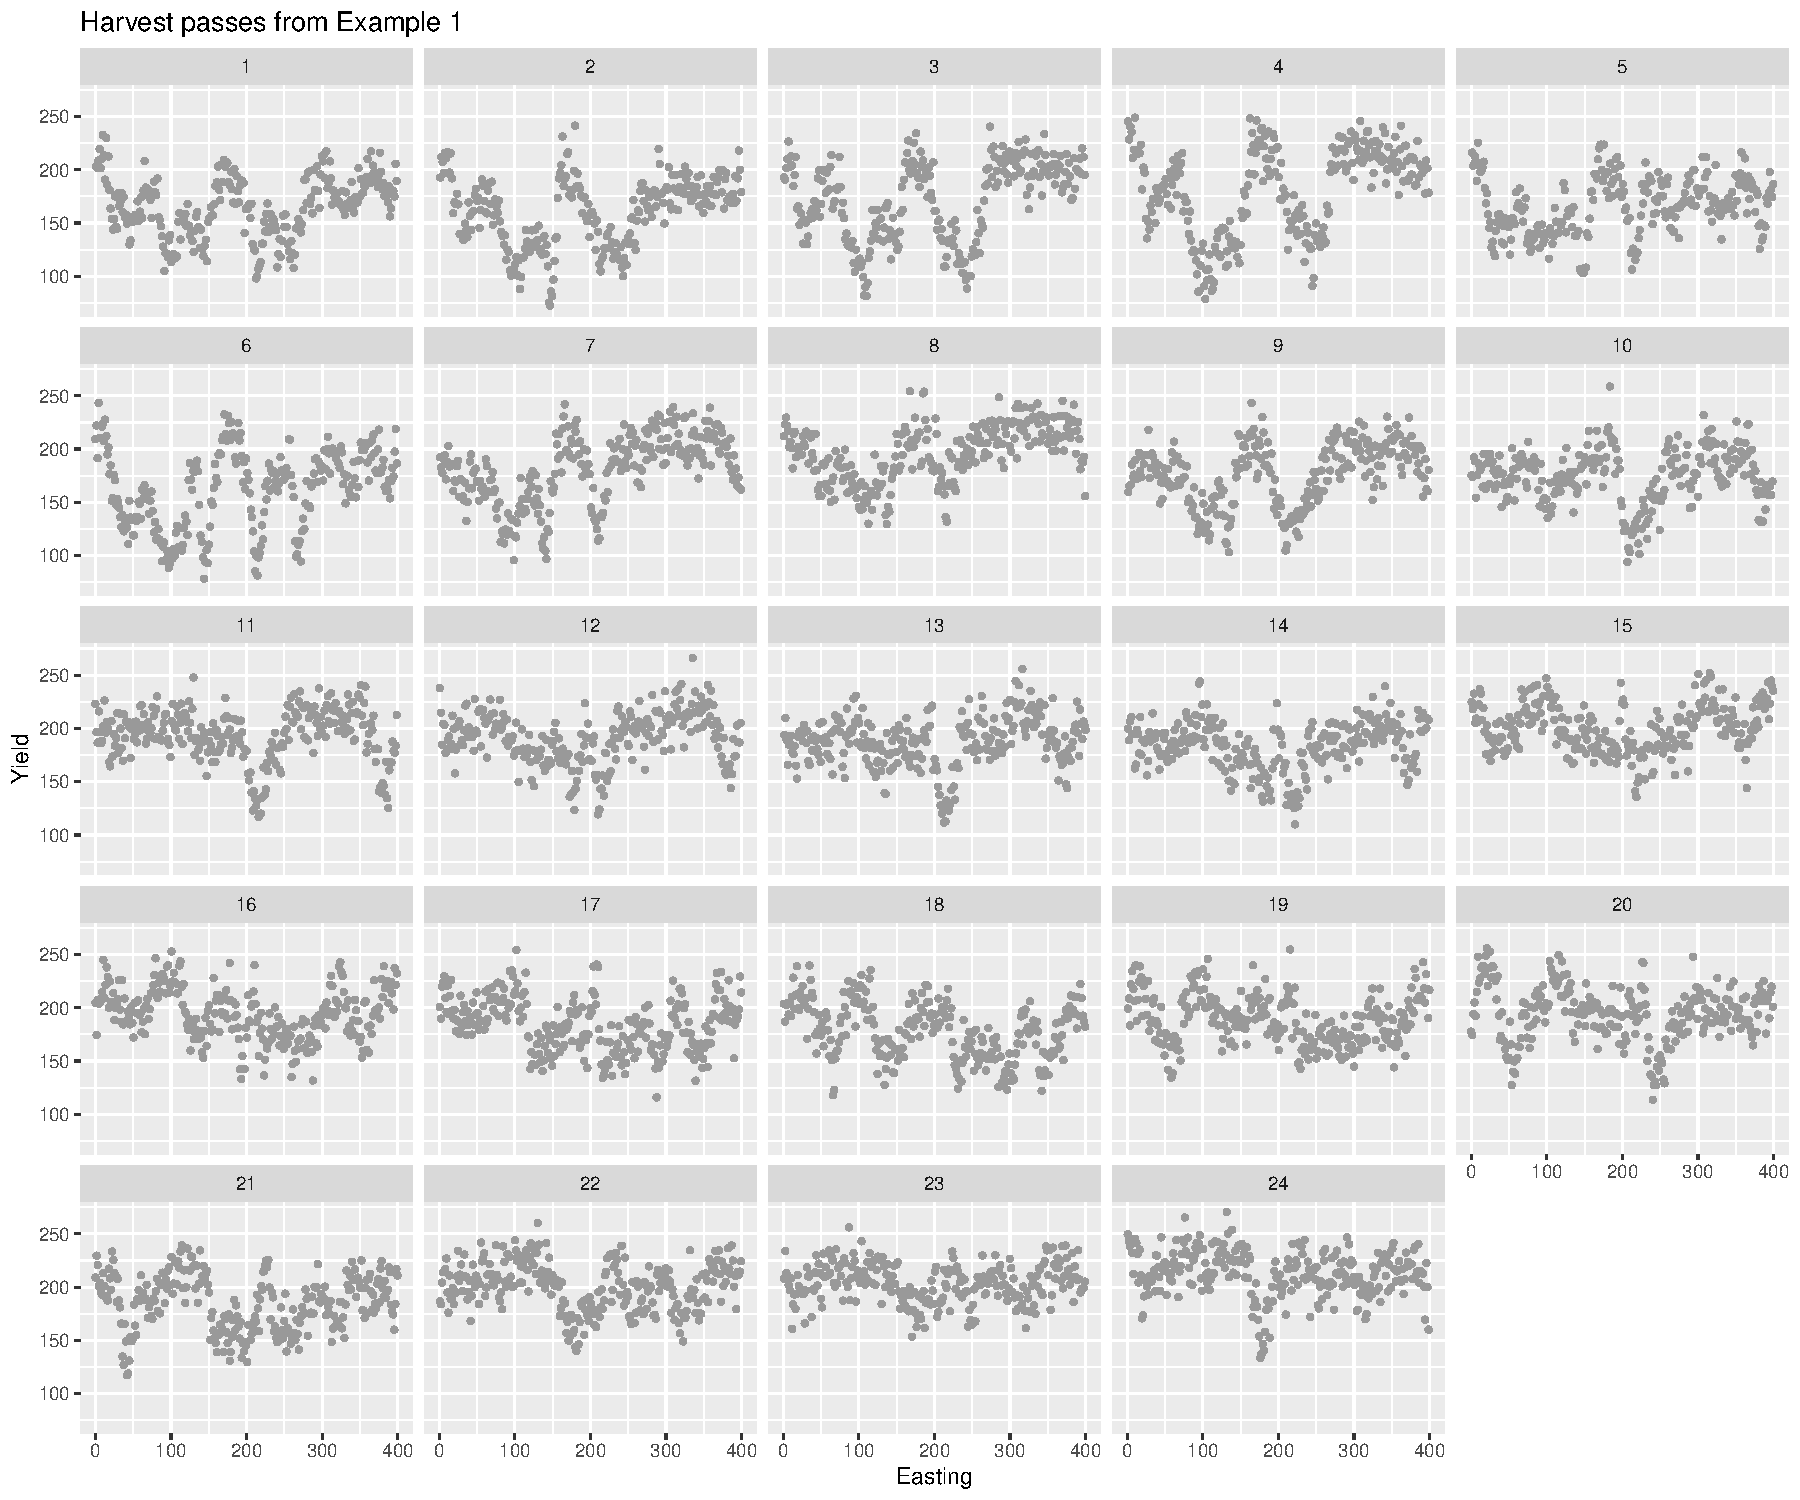
\includegraphics{Thesis-RawSwaths}
\caption{Harvest passes with no smoothing. For the first example data set, there are 24 sets of instantaneous yield points to be smoothed an interpolated by functional forms. See Figure \ref{RawSwath} for more details}\label{RawSwaths}. 
\end{figure}

To provide a context for the extent of the problem of finding functional forms for observational units (harvest passes) in a single strip trial, the yield observations from Example 1 are considered, plotted by position of the observation (\texttt{Easting}) grouped by harvest pass number (\ref{RawSwaths}). As seen in following sections, key parts of finding a functional form for these data is choosing a functional basis for these data, then identifying an appropriate degree of smoothness for the functional basis. If there were no time constraints, each harvest pass could be fit individually, finding the unique combination of basis functions and smoothing parameters optimal for each harvest pass. However, it is assumed that obtaining unique solutions for each harvest pass is impractical, and I will, in this section, attempt to determine if there is an implementation of smoothing functions such that the default behavior of the fitting library provides a solution sufficient for all harvest passes in these data without fine-tuning smoothing parameters. Methods for automating the process will be suggested in this thesis.

\clearpage

\section{Smoothing functions for a single observational unit}


\begin{figure}\centering
\includegraphics{Thesis-RawSwath}
\caption{Representative harvest pass with no smoothing. These data are the 24$^{th}$ or northern most harvest pass shown in Figure \ref{RawSwaths}. Instantaneous yield estimates are shown as gray points. Yield estimates are taken a 1 second intervals, but it is the location of estimates that is of primary interest, so points are plotted versus meters \texttt{Easting}}\label{RawSwath}
\end{figure}

To illustrate different methods of fitting functional forms to data an example a single harvest pass taken from Example 1 (Section \ref{Example1Section}). The last harvest pass of the data (pass number 24) has been selected arbitrarily. The original yield observations for this harvest pass are shown in Figure \ref{RawSwath}.

Consider Figure \ref{RawSwath} as a single specific instance of some $y_{ij}$ The goal here to find an smoothing function $f$ that minimizes deviations from the true data generating process $F$ and maps data samples at uniform time intervals to a uniform set of distance points, while preserving the features of the original data. Specifically, in the case of \ref{RawSwath}, inspection of the data leads to the following features: A decrease from approximately 240 $bu/ac$ over the first 10m followed by a rise that appears to end at about 80m. There may be a slight decrease in yield from 80m to 110m, but yield appears stable from 110m to 160m. At 160m, there is an abrupt decrease in yield which rises to a more stable yield at about 210m. There may be small fluctuations in yield from 210m to 300m, where there appears to be a small decrease in yield from 300m to 330m, then yield appears stable until a possible decrease at 400m. A functional representation of the data should reflect the features found by visual inspection of the raw data.

Choosing an appropriate function $f$ is part of the art of functional analysis. The choice of function is largely going to depend on the relative importance placed on two components of the functional form - smoothing and interpolation. Functional data are in theory continuous values, but data are commonly collected at discrete intervals, and measurement errors occur during when functions are sampled. Smoothing occurs when functional forms are chosen to minimize variance between the function values at sample points and the sampled values.

%A generalized additive model following from our previous examples may take the form (adapted from \cite{wood-2017} )

%\begin{equation}
%g(y_i) = \mathbf{A_i} \mathbf{\theta} + f(x_{1i}) +f(x_{2i},x_{3i}) + e_i
%\end{equation}

%where $\mathbf{A_i} \mathbf{\theta}$ are the strictly parametric components of the model and  $f(\circ)$ is a function form of the covariate $x_1, \dots$. In the functional analysis of strip trials, $\mathbf{A_i} \mathbf{\theta}$ would represent the treatment structure while $f(x_{1i})$ represents a smooth function of yield over distance.

%In this case, we can assume $g(y_i)=y_i$ and $\mathbf{A_i} \mathbf{\theta} = \mu_i$, so this simplifies to a linear model with respect to the smoothing function. We will use distance from the a fixed end of the field as covariate $x = x_1$

%\begin{equation}
%y_i = f(x) + e_i
%\end{equation}

%\section{Forms of $f(x)$}

%The choice of $f(x)$ depends largely on a smoothing parameter $\lambda$ that determines how 'smooth' or 'wiggly' the resulting interpolating function fits the data. Too smooth and the data are under fit, losing information. If the fit is too rough and the data are over fit, including too much error variance in the model. We use the R library \texttt{mgcv} to perform generalized cross-validation \cite{wood-2017}, p 169, of the fitted function $f_i(x)$ to obtain an appropriately smooth $f_i(x)$. Fitted values are then taken as the true yield at point $x$, and this value is used to compute summary statistics for functional data analysis. 

\clearpage

\section{Representing $f$}

To simplify discussion in this next section, only a single functional variable $y$ will be considered, dropping the $ij$ subscript notation. Following \cite{wood-2017}, represent a simple smoothing function of one covariate as
\begin{equation}
y_i = f(x_i) + e_i
\end{equation}\label{SimpleFunctionalForm}
where $y$ is the response variable, $x$ is a covariate, $f$ is a smooth function and the $e_i$ are normally distributed random variables. In this context, the function $F$ that generates the data in Figure \ref{RawSwath} is represented as an computational form $f$.

Several mathematical models exist that are used to approximate $f$. In this section some possible functional forms are reviewed, again following \cite{wood-2017}, p. 162. Define a \textit{basis} as a space of functions which includes $f$, which represents a fuctional representatition of $$F$$ as an element. Ideally, $f$ is an optimal approxatiomation of $F$, by some definition or optimal. There are different methods for choosing optimality. A basis is defined by some set of functions $b_j(x)$, $j = 1, \cdots, k$. Represent $f$ as a sum of the basis functions,
\begin{equation}
f(x) = \sum_{j=1}^k \beta_j b_j(x)
\end{equation}\label{GenericBasisFunctions}
with $\beta_j$ being unknown parameters to be found from data. Rewrite this in matrix form as
\begin{equation}
f(\mathbf{x}) = \mathbf{X} \mathbf{\beta}
\end{equation}\label{BasisFunctionsMatrixForm}
where $X_{ij} = b_{j}(x_{i})$ and $\mathbf{\beta} = \left\{\beta_1, \beta_2, \cdots \right\}$

\clearpage

\subsection{Polynomial functions}

Polynomial functions are frequently used as functional forms due to their simplicity and flexibility. Unlike power or exponential functions, polynomial functions can be fit to data using ordinary least squares (polynomial regression), while any number of data points can be fit exactly using polynomials of sufficiently high order.

Polynomial functions take the form
\begin{equation}
f(x_i) = \beta_0 + \beta_{1} x + \dots + \beta_{k} x_i^k
\end{equation}
where $k$ is the order of the polynomial. Clearly, a polynomial function forms a basis. Write the polynomial function as
\begin{equation}
f(x) = \sum_{j=1}^{k+1} \beta_{j} x^{j-1}
\end{equation}

 
\begin{figure}\centering
\includegraphics{Thesis-PolynomialSmoothing}
\caption{Interpolation of yield points using a linear model of degree 12. Instantaneous yield estimates are shown in gray lines, while a polynomial curve of degree twelve smoothing the points is shown as a line.}\label{PolynomialSmoothing}
\end{figure}

Figure \ref{PolynomialSmoothing} show a polynomial of order 12 superimposed over the original data. This function in general smoothly interpolates the data, but does over-smooth the key feature at 180m. 

\subsection{Local smoothing}

\begin{figure}\centering
\includegraphics{Thesis-SeveralPolynomials}
\caption{Smoothing the raw data with polynomials of increasing order. Instantaneous yield estimates are shown by gray points, and polynomial functions interpolating and smoothing these points are shown as lines}\label{SeveralPolynomials}
\end{figure}


A problem with polynomial regression is the regression is by definition global; the entire range of $x_i$ is fit by a single function This may allow for non-local influences. Data in one region, particularly points with unusual leverage, can influence the fit in other regions of the data \cite{fox-1997}. The order $k=12$ for Figure \ref{PolynomialSmoothing} was chosen after some trial and error. If increasing the the order of the polynomial, dramatic oscillations in what appear by inspection to be relatively smooth parts of the original data can be seen in Figure \ref{SeveralPolynomials}.

%Thus, any midpoint value between two arbitrary points $x_i$ and $x_i$ can be interpolated exactly with a polynomial of order 1. i.e $y = a +bx_i$. One possible functional form for $y_{ij}$, then, computes $y(d)$ for any $d$ by identifying the $y_{ikK}$ bounding $d$ and finding the straight line interpolation between the points.

An alternative approach, piecewise linear regression, partitions the data into \textit{bins} defined by a set of endpoints for each bin or \textit{knots} \cite{wood-2017}. Multiple linear models result, each restricted to a bin \cite{fox-1997}. Bins, and thus the individual linear models, are joined at the knots. The basis for this interpolation is a series of simple linear function.

Let the knots be represented as ${x^{*}_j} : j = 1, \cdots, k$ such that $x^{*}_j>x^{*}_{j-1}$. For $j=2,\cdots, k-1$,  The basis functions of a \textit{piecewise} linear interpolation \cite{wood-2017} can be represented as
\begin{equation}
b_j(x) = 
  \begin{cases} 
      (x-x^{*}_{j-1})/(x^{*}_j-x^{*}_{j-1}) &  x^{*}_{j-1} < x \le x^{*}_{j} \\
      (x^{*}_{j+1}-x)/(x^{*}_{j+1}-x^{*}_{j}) & x^{*}_{j} < x \le x^{*}_{j+1} \\
      0 & \text{otherwise}
   \end{cases}
\end{equation}\label{PiecewiseLinearBasis}
with 
\begin{equation}
b_1(x) =
\begin{cases}
(x^{*}_2-x)/(x^{*}_2 - x^{*}_1) & x < x^{*}_2 \\
0 & \text{otherwise}
\end{cases}
\end{equation}
and
\begin{equation}
b_k(x) =
\begin{cases}
(x - x^{*}_{k-1})/(x^{*}_k - x^{*}_{k-1} ) & x > x^{*}_{k-1} \\
0 & \text{otherwise}
\end{cases}
\end{equation}

\begin{figure}\centering
\begin{Schunk}
\begin{Soutput}
$x
[1] "Easting"

$y
[1] "Yield"

$title
[1] "Single harvest pass, piecewise linear interpolation"

attr(,"class")
[1] "labels"
\end{Soutput}
\end{Schunk}
\includegraphics{Thesis-PiecewiseLinear}
\caption{Piecewise linear interpolation. Instantaneous yield estimates (shown as gray points) are interpolated by a set of short linear curves. There are 12 knots specified for this interpolation, resulting in 11 linear basis functions. The number of knots in this curve was deemed optimal by inspection.}\label{PiecewiseLinear}
\end{figure}

Figure \ref{PiecewiseLinear} shows piecewise linear regression superimposed on the observed harvest values for the example strip data. With 12 knots, piecewise linear regression appears to preserve key features of the original data. However, the choice of knots was be made by inspection; there was no automated method for choosing knots. Code for this figure was adapted from \cite{wood-2017}. We will use the same number of knots in Figure \ref{ComparingSplineFits}

%Piecewise <- data.frame(
%  Easting = seq(min(x), max(x) ,len = 10000)
%)
%Piecewise[,'Yield'] <- predict(model, newdata = data.frame(x = Piecewise[,'Easting']))
%Knots = data.frame(
%  Easting = seq(min(x), max(x), len = K + 2)[-c(1, K + 2)]
%)
%Knots[,'Yield']  = predict(model, newdata = data.frame(x = Knots[,'Easting']))
                           
%ggplot(SinglePass.dat, aes(Easting,Yield)) + 
%   geom_line(linewidth=1,color=cbPalette[1]) + 
%   #geom_point(size=1,color=cbPalette[1]) + 
%   geom_line(aes(Easting,Yield),linewidth=1,color=cbPalette[2],data=Piecewise) +
%   geom_point(size=2,color=cbPalette[2],data=Knots) 

\clearpage

\subsection{Spline basis functions}

Although smoothing functions, such as a Fourier series \cite{schoenberg-04-1946} for data have been discussed historically, this thesis is limited exploration to smoothing functions commonly referred to as \textit{splines} \cite{perperoglou-2019}.  As with the piece wise regression model, spline models are commonly piecewise and constrained to be continuous at the knots. Most splines also have the constraint that the first and second derivatives are also continuous; and in most cases cubic splines are used, such that a cubic polynomial interpolates the region between knots \cite{perperoglou-2019}.

%Following \cite{perperoglou-2019}, a cubic spline function with three knots $x^{*}_1, x^{*}_2$ and $x^{*}_3$ can be represented as
%\begin{equation}
%f(x) = \beta_0 + \beta_1 x + \beta_2 x^2 + \beta_3 x^3 + \beta_4(x-x^{*}_1)^3 + \beta_5(x-x^{*}_2)^2 + \beta_6(x-x^{*}_3)^3
%\end{equation}

\cite{wood-2017} p. 201 defines a cubic spline function $f(x)$ with $k$ knots, $x_1, \cdots x_k$, as
\begin{equation}
f(x) = a^-_j(x)f(x_j) + a^+_j(x) f(x_{j+1}) + c^-_j(x) f''(x_j) + c^+_j f''(x_{j+1}) \text{ if } x_j \le x \le x_{j+1}
\end{equation}
where 
\begin{equation}
\begin{aligned}
a^-_j(x) &= (x_{j+1}-x)/(x_{j+1}-x_{j}) \\
a^+_j(x) &= (x-x_j)/(x_{j+1}-x_{j}) \\
c^-_j(x) &= \left[ (x_{j+1} - x)^3/(x_{j+1}-x_{j}) - (x_{j+1}-x_{j})^2 \right] / 6\\
c^+_j(x) &= \left[ (x-x_j)^3/(x_{j+1}-x_{j}) - (x_{j+1}-x_{j})(x-x_j)\right] / 6\\
\end{aligned}
\end{equation}

(Note that for this discussion, we use the notation $x_i$ to represent sampling points from data, while $x_j$ identify the position of knots)

Suppose knots are defined by ${x_i, y_i : i=1,..,n}$. The natural cubic spline $g(x)$ is defined as a function over the bins defined by $[x_j, x_{j+1}]$ where a cubic polynomial interpolates over each bin \cite{wood-2017}. The knots are joined in such a way as the whole spline is continuous to the second derivative, where $g(x_i)=y_i$, while $g''(x_1) = g''(x_n) = 0$. Natural splines with $k$ knots will have $k+1$ degrees of freedom; the number of splines, minus one plus the two constraints the the second derivative \cite{perperoglou-2019}.

B-splines are an alternative representation of a spline basis \cite{wood-2017, perperoglou-2019}. Define $m+1$ as the order of the basis (so, for a cubic spline $m=2$). B-splines are non-zero over the interval between $m+3$ knots, so are less local than ordinary splines. A $k$ parameter b-spline is defined over $k+m+2$ knots\cite{wood-2017}, so b-splines have $p+k$ degrees of freedom \cite{perperoglou-2019}, where for cubic splines $p=3$. Restated, b-splines with $d.f.$ degrees of freedom will have $d.f.-3$ knots in the case of a cubic spline basis.

An $(m+1)^{th}$ order b-spline takes the form 
\begin{equation}
f(x) = \sum_{i=j}^k B^m_j(x) \beta_j
\end{equation}

The basis functions for b-splines are typically defined recursively \cite{wood-2017, perperoglou-2019}, taking the form \cite{wood-2017}
\begin{equation}
   B_j^m(x) = \frac{x-x_j}{x_j+m+1}B^{m-1}(x) + \frac{x_{j+m+2}-x}{x_{i+m+2}-x_j+1}B^{m-1}_{j+1}(x), i = 1, \cdots, k
\end{equation}
with
\begin{equation}
   B^{-1}_j(x) = 
   \begin{cases} 
      1 & x_j \leq x < x_{j+1} \\
      0 & otherwise
   \end{cases}
\end{equation}

Extending the b-spline are p-splines \cite{eilers-1996}. Note that both natural splines and b-splines are commonly fit using ordinary least squares regression, by minimizing an objective function taking the form
\begin{equation}\label{OLSObjective}
S = \sum_{i=1}^m \left\{  y_i - \sum_{j=1}^n \beta_j B_j(x_i) \right\}^2
\end{equation}

In contrast, solutions for p-splines involve some version of a penalty function in addition to the ordinary least squares penalty in Equation \ref{OLSObjective}. The ordinary least squares penalty is named as such because solutions found using this penalty minimize the sum of squared differences between the observed values and the predicted values. Equation \ref{OLSObjective} is frequently written as in Equation \ref{OLSModel}.

P-splines has become a somewhat generic term for splines \cite{eilers-09-2010} where the objective function contains an additional penalty function that adjusts for the smoothness of the spline. For example, \cite{eilers-1996} add a finite difference penalty, so that the function to be minimized takes the form
\begin{equation}\label{PBsplines}
S = \sum_{i=1}^m \left\{  y_i - \sum_{j=1}^n \beta_j B_j(x_i) \right\}^2 + \lambda \sum_{j=k+1}^n (\Delta^k \beta_j)^2
\end{equation}
where $\lambda$ is a tuning parameter to control the degree of penalization, and ultimately the \textit{wiggliness} allowed when fitting the splines. \cite{eilers-09-2010} have taken a preference to refer this form as the PB-spline. In the same reference, \cite{eilers-09-2010} refer to a PT-spline. PT-splines are not explicity used in in this thesis, so this thesis leaves out the mathematics in detail, but simply state that PT-splines include essentially a ridge-regression penalty. In \texttt{mgcv}, \cite{wood-2017} implements a penalized spline (\texttt{bs='ps'}) where the penalty is a \textit{difference penalty} applied to coefficients of $\mathbf{\beta}$, written as
\begin{equation}\label{WoodPS}
\mathcal{P} = \sum_{i=1}^{k-1} \left( \beta_{i+1} - \beta_{i} \right)^2
\end{equation}

Note that the \cite{wood-2017} version of penalized splines (Formula \ref{WoodPS}) is similar to, but simpler than, the version labeled PB-splines by \cite{eilers-1996} (Formula \ref{PBsplines}). Regardless of penalty function, penalized splines are typically based on b-splines, so for $k+4$ degrees of freedom fit using \texttt{mgcv} it would be expected that there are $k$ knots for penalized splines. With other packages, the relationship between knots and degrees of freedom would be expected to be $d.f. = knots+3$

The \texttt{mgcv} library will be used extensively in this thesis. Thin-plate splines \cite{wood-2003} are a form of penalized splines that provide a general solution to smoothing functions of multiple variables \cite{wood-2017}. In a general sense, \cite{wood-2003} discusses splines on data of arbitrary dimension by describing the smoothness penalty as
\begin{equation}
   \lambda \int \dots \int_{\mathcal{R}^d}
   \sum_{\nu_1 + \dots + \nu_d = m} 
   \frac{m!}{\nu_1 ! \dots \nu_d !}
   \left( \frac{\partial ^m g}{\partial x_1^{\nu_1} \dots \partial x_d^{\nu_d}}\right)^2
   dx_1 \dots d x_d
\end{equation}
where $\lambda$ controls the contribution of the penalty function to the objective function as in Equation \ref{SmoothingSplinePenalty}.

In this thesis the number of covariates is limited to two; this implies a smoothness penalty, using second derivatives to be comparable to Equation \ref{SmoothingSplinePenalty}, can be written \cite{wood-2017} as
\begin{equation}\label{Thinplate2}
   \lambda \int \int \left( \frac{\partial^2 f}{\partial x_1^2}\right)^2  +
              2 \left( \frac{\partial^2 f}{\partial x_1 \partial x_2} \right) +
              \left( \frac{\partial^2 f}{\partial x_2^2}\right)^2 d x_1 d x_2
\end{equation}

Written in this form, we can see that the penalty for thin-plate splines simplifies the penalty in Equation \ref{SmoothingSplinePenalty}. It is common to see thin-plate splines extended to non-planar surfaces \cite{bookstein-06-1989, keller-02-2019}. 


A further extension to penalized splines allows the penalty to be weighted according to the covariate $x$. \cite{wood-2017} refers to these as adaptive splines. The penalty function is similar to Equation \ref{WoodPS}, with the addition of a weight vector $\mathbf{\omega}$ that varies with $i$. Wood \cite{wood-2017} writes this in the form of a second-order P-spline, but for simple a simple first-difference penalized spline as in Equation \ref{WoodPS}, the penalty takes the form
\begin{equation}\label{WoodAD}
\mathcal{P} = \sum_{i=1}^{k-1} \omega_i \left( \beta_{i+1} - \beta_{i} \right)^2
\end{equation}.
Wood \cite{wood-2017} states that the weights $\omega_i$ vary smoothly with $i$, and claims that the obvious $\omega_i$ is computed using a B-spline expansion, resulting in a multiply penalized b-spline. As shown in Figure \ref{ComparingGAMSplines}, adaptive splines as implemented by the \texttt{mgcv} library tend to default to be more wiggly than other spline families, and require large numbers of knots (Figure \ref{PredictionsGAMAD}).

In a more general sense, the term \textit{adaptive} splines refers to splines where the basis is not a fixed set of knots, but instead is determined by the data \cite{mammen-1997}. A version of this can be found in the \texttt{aspline} library in R, but comparison of adaptive splines is beyond the scope of this thesis.

\clearpage

\section{Fitting splines in R}

There exists a variety of libraries and functions in R that may be used to interpolate or smooth noisy data using spline functions \cite{perperoglou-2019}. The applicability of some of the functions to the example harvest strip will be considereed using the data in Figure \ref{RawSwath}

\subsection{Spline interpolation using simple linear regression}

Let $\mathbf{X}$ be a design matrix encoding spline coefficients ($b_j$) from equation \ref{GenericBasisFunctions}, such that the problem of fitting a set of spline basis functions reduces to the problem of minimizing 
\begin{equation}\label{OLSModel}
\lVert\mathbf{y} - \mathbf{X} \mathbf{\beta} \rVert ^2,
\end{equation}
 
where $\mathbf{y}$ is the vector of $y_i$ from Equation \ref{SimpleFunctionalForm} while $\mathbf{X}$ and $\mathbf{beta}$ are from Equation \ref{BasisFunctionsMatrixForm}. The solution vector $\widehat{\beta}$ can be found using ordinary least squares. The \texttt{lm} function in R is used to compute a least squares solution to problems of form of Equation \ref{OLSModel}.

Splines are expanded to appropriate $\mathbf{X}$ matrices representing a function form the data using the \texttt{spline} \cite{rcore} library in R and coefficients are found using the \texttt{lm} function. The \texttt{spline} library includes two functions that expand to spline bases, \texttt{ns} and \texttt{bs}. \texttt{ns} produces the basis matrix for natural splines, while \texttt{bs} produces the basis matrix for b-splines. 

The \texttt{ns} function accepts \texttt{df} as an argument to controlling smoothness and the function chooses \texttt{df - 1} knots. For illustration, the argument \texttt{df=12+1}, so the resulting spline bases has 12 knots, comparable to the piecewise linear fit in Figure \ref{PiecewiseLinear}

\texttt{bs} chooses \texttt{df-degree} number of knots if \texttt{df} is passed an a argument. That is, the \texttt{bs} function called using the argument \texttt{df=15} will generate 12 knots . B-splines with \texttt{12+3=15} degrees of freedom identifies similar features as with \texttt{ns} with \texttt{12+1 = 13} degrees of freedom (Figure \ref{ComparingSplineFits}).

In both cases, the \texttt{lm} function computes $\widehat{\beta}$ from the unpenalized objective function in Formula \ref{OLSModel}


\begin{figure}\centering
\includegraphics{Thesis-NSBasisPlot}
\caption{Basis values from the $X$ design matrix for the spline \texttt{ns(df=13)} used to illustrate the natural spline fit with 12 knots in Figure \ref{ComparingSplineFits}. Each line represents a column in $X$, and the \texttt{lm} model fit finds a $\beta$ that best fits the data. This figure shows that each column of $X$ is largely zeros, except for the region defined by the basis function (which are defined by the knots). The values in the $X$ matrix are coefficients appropriate to produce a cubic polynomial over the interval defined by the region between knots, with some overlap between basis functions at the knots. This plot does not seem appropriate for natural splines, since the endpoints are not symmetrical. It is not clear from the help topic for \texttt{ns} why this should be so.}\label{NSBasisPlot}
\end{figure}


\begin{figure}\centering
\includegraphics{Thesis-BSBasisPlot}
\caption{Basis values from the $X$ design matrix for the spline \texttt{bs(df=15)} used to illustrate the basis spline fit with 12 knots in Figure \ref{ComparingSplineFits}. See Figure \ref{NSBasisPlot} for a description of the lines. Columns 4-13 define simple bell-shaped curves similar to those shown in Figure \ref{NSBasisPlot}, while columns 2, 3, 14 and 15 define skewed bell curves at endpoints of the range of $x_j$ and column 1 is a constant or intercept} \label{BSBasisPlot}.
\end{figure}

To illustrate the concept of basis functions easily with design matrices \texttt{X}, first \texttt{X} matrices are extract from the object returned by \texttt{lm}. It is not so convenient to show the basis functions fit using \texttt{mgcv}, so only the basis functions for the \texttt{splines} fit using \texttt{lm} are shown in Figures \ref{NSBasisPlot} and \ref{BSBasisPlot}. Only the bases functions in \ref{BSBasisPlot} will be used to illustrate the process of combining bases functions to producs a smooth functional form. Let $\mathbf{y} = \mathbf{X} \mathbf{\beta}$. Figure \ref{BSBasisPlot} shows the \texttt{X} matrix expanded from the \texttt{bs} function. \cite{ramsay-2005} makes the point that B-splines are cubic splines with the support of each spline on the interval $[\tau_{k-2}, \tau_{k=2}]$; that is, the sample points where the basis function is non-zero extends beyond the boundary knots for the basis function.

\begin{figure}\centering
\includegraphics{Thesis-BSBasisPlot2}
\caption{Basis values from the as shown in Figure \ref{BSBasisPlot} multiplied by the corresponding \texttt{lm} coefficients. Note that most of the basis values appear negative when multiplied by coefficients from the \texttt{lm}. This is likely due to the large intercept value at ~ 250 bu/acre, and the functional form of these data is found by subtracting from the intercept.} \label{BSBasisPlot2}
\end{figure}

Consider the \texttt{bs} basis functions and resulting functional form in more detail. In mathematical notation, let $x_1, x_2, \dots x_n$ be the sample points for the data in Figure \ref{RawSwath} and $X_{1,1}, X_{2,1}, \dots, X_{k,1}$ be the non-zero elements of first column \texttt{X} with $X_{k+1,1} = X_{k+2,1} = \dots X_{n,1} = 0$. More generally, the values in \texttt{X} will be the basis functions evaluated at the sampling ponts, in the case of b-splines ths will be of the form $X_{i,j} = B^m_j(x_i)$. The values $X_{1,1}, X_{2,1}, \dots, X_{k,1}, X_{k+1,1}, X_{k+2,1}, \dots X_{n,1}$ are plotted as the second curve in Figure \ref{BSBasisPlot}, while  are plotted in Figure 

Multiply each basis column by it's associated estimated $\widehat{\mathbf{\beta}}$ coefficients, that is, $\beta_{1} X_{1,1}, \beta_{1} X_{2,1}, \dots, \beta_{1} X_{k,1}, \beta_{1} X_{k+1,1}, \beta_{1} X_{k+2,1}, \dots \beta_{1} X_{n,1}$. $\widehat{\mathbf{\beta}}$ extracted from the associated \texttt{lm} object using the \texttt{coef} function. These curves are shown in Figure \ref{BSBasisPlot2}. Next, summing over all $X$ rows for each sampling point $x_i$. This can be achieved by multiplying the design matrix $X$ by the coefficients $\widehat{\beta}$ and plotting $\widehat{y_i}$ against $x_i$, as show in Figure \ref{BSBasisPlot3}. This reproduces the curve shown in Figure \ref{ComparingSplineFits}.

\begin{figure}\centering
\includegraphics{Thesis-BSBasisPlot3}
\caption{Predicted values by summing over data points, using the form $\widehat{y} = X \widehat\beta$, where $X$ is illustrated in Figure \ref{BSBasisPlot} and $\widehat{\beta}$ is obtained from the \texttt{lm} function as used to generate the \texttt{lm bs, df = 12+3} curve from Figure \ref{ComparingSplineFits}} \label{BSBasisPlot3}
\end{figure}

\clearpage

\subsection{b-splines for functional data}

The R library \texttt{fda} is popular for functional data analysis \cite{ramsay-2009}. In particular, the \texttt{fda} library provides a function for producing b-spline basis functions. However, in general this function, \texttt{create.bspline.basis} requires many more arguments such as an explicit set of knots and an order for the basis functions (as opposed to assuming a cubic spline basis). The use of \texttt{create.bspline.basis} is demonstrated in Figures \ref{PredictionsFDA} and \ref{SplitsCompOCV} because the \texttt{fda} library that may be of use in some of the problems with yield monitor data, particularly the alignment problem. However, the flexibility of \texttt{fda} library comes at the expense of usability. Further, I have interest in combining smoothing functions with estimates of fixed effects; for that I turn to generalized additive models.

%## Smoothing Penalty

%In the previous examples, coefficients $\beta_i$ are estimated using ordinary least squares; that is, coefficients are found that minimize \cite{craven-1979]
%$$
%\frac{1}{n} \sum_{j=1}^n (f(x_j) -y_j)^2
%$$
%To estimate an optimal amount of smoothing, a penalty is introduced \cite{craven-1979]. The frequently takes the form
%$$
%\frac{1}{n} \sum_{j=1}^n (f(x_j) -y_j)^2 + \lambda \int_0^1(f^{(m)}(u))^2 du
%$$
%\cite{craven-1979] uses the notation $g_{n, \lambda}$ where $g \in W_2^(m)= {f: f,f', \cdots, f^{m-1} abs. cont., f^{(m)} \in \mathcal{L}_2[0,1]}$.

\subsection{Fitting splines}

In this section libraries for fitting splines are compared with libraries for fitting generalized additive models, specifically generalized additive models without fixed effects. Generalized additive models with fixed effects will be considered in Chapters \ref{TrendAnalysisChapter} and \ref{SpatialAnalysisChapter}.

In the broad sense, a generalized additive model takes the form (adapted from \cite{wood-2017})
\begin{equation}\label{GAMFormula}
g(y_i) = \mathbf{A_i} \mathbf{\theta} + f(x_{1}) + f(x_2, x_3) + e_i
\end{equation}
where $\mathbf{A_i} \mathbf{\theta}$ are the strictly fixed effects or parametric components of the model and  $f(x_i,\cdots)$ is a function form of the covariate(s) $x_i, \cdots$. 

In this case, assume $g(y_i)=y_i$ and $\mathbf{A_i} \mathbf{\theta} = \mu_i$, so this simplifies to a linear model with respect to the smoothing function, thus is of the form $y_i = f(x) + e_i$

Now, reconsider the piecewise linear basis in Equation \ref{PiecewiseLinearBasis}. Instead of minimizing $\lVert\mathbf{y} - \mathbf{X} \mathbf{\beta} \rVert ^2$, the wiggliness of the resulting fit model can be controlled the by minimizing a penalized objective function \cite{wood-2017}
\begin{equation}\label{PiecewisePenalized}
   \lVert\mathbf{y} - \mathbf{X} \mathbf{\beta} \rVert ^2 + \lambda \sum_{j=2}^{k-1} \left\{f(x^*_{j-1})-f(x^*_j) + f(x^*_{j+1})  \right\}^2
\end{equation}

This adds, as sum of squared second differences of the function at the knots, to the simpler linear sums of squares penalty function; when the basis functions are splines this can be represented by the second integral of the smoothing function,
\begin{equation}\label{SmoothingSplinePenalty}
   \sum_{i=1}^n\left\{ y_i -f(x_i) \right\}^2 + \lambda \int f''(x)^2 dx
\end{equation}.
The form of a penalized function is common in the literature, and is sometime simply referred to as \textit{smoothing} splines \cite{hastie-2010}. 

In either case, the wiggliness of the smoothing function relative to the data can be controlled by the selection of $\lambda$. That is, given an estimate $f$ of the true data generative function $F$, large values of $\lambda$ over-smooth the data, while small values of $\lambda$ under-smooth the data, in either case resulting in an estimated $f$ that is not close to the true value $F$ \cite{wood-2017}. Ideally, $f$ would be chosen such that the value
\begin{equation}
   M = \frac{1}{n} \sum_{i=1}^n (F(x_i)-f(x_i))^2
\end{equation}
is minimized. Clearly, $f$ cannot directly measured, so $M$ cannot be computed directly. However, the expected squared error of predicting a new variable, $\mathbb{E}(M)+\sigma^2$, can be estimated. Let $f^{[-i]}$ be the value of $f$ fit to all the $\mathbf{y}$ except the single value $y_i$. Wood \cite{wood-2017} then defines the ordinary cross validation score as

\begin{equation}\label{OrdinaryCrossValidation}
\mathcal{V}_0 = \frac{1}{n} \sum_{i=1}^n (f^{[-i]}(x_i) - y_i)^2
\end{equation}

Now, $f^{[-i]} \approx F$ when $n$ is sufficient large, and it can be shown \cite{wood-2017} that $\mathbb{E}(\mathcal{V}_0) \approx \mathbb{M}+\sigma^2$, again for sufficiently large $n$. This leads to the conclusion that $M$ can be minimized by choosing a $\lambda$ that minimizes $\mathcal{V}_0$. However, especially for large $n$ (or correspondingly $f$ with a large number of free parameters) computing $\mathcal{V}_0$ directly is computationally expensive. However, is can also be shown \cite{wood-2017} that

\begin{equation}\label{OrdinaryCrossValidationInfluence}
\mathcal{V}_0 = \frac{1}{n} \sum_{i=1}^n (y_i - f(x_i))^2 / (1-A_{ii})^2
\end{equation}

where $f$ is fit to the entire data set, and $\left\{ A_{ii} \right\} = \mathbf{A}$ is the influence matrix for $\widehat{f}$. $\mathbf{A}$ is computed as
\begin{equation}\label{InfluenceMatrix}
\mathbf{A} = \mathbf{X} \left( \mathbf{X}^t \mathbf{X} + \lambda \mathbf{S} \right)^{-1} \mathbf{X}^t   
\end{equation} with $\mathbf{S} = \mathbf{D}^t \mathbf{D}$ where $\mathbf{D}$ is formed from the columns of $\mathbf{X}$ \cite{wood-2017}.

This leads to a generalized cross validation score

\begin{equation}\label{GeneralizedCrossValidation}
\mathcal{V}_g = \frac{n\sum_{i=1}^n (y_i - f(x_i))^2}{[n-tr(\mathbf{A})]^2}
\end{equation}

The takeaway from this is that when a model is fit using \texttt{mgcv}, the user does not need to select $\lambda$, instead \texttt{mgcv} finds a a value of $\lambda$ that minimizes the generalized cross validation score. From this, the objective function in Formula  \ref{SmoothingSplinePenalty} is use to find the coefficients of the basis functions $\widehat{\beta}$; the number of basis functions is held constant.

In other cases the generalized cross validation score is used to select the number of knots for a penalized spline function \cite{friedman-02-1989, ruppert-01-2002}. This does not seem to be the case for the library \texttt{mgcv}; the number of knots found when a penalized spline is required (\texttt{bs='ps'}) defaults to the same number of knots found when the basis argument is \texttt{bs='bs'}, as discussed below.

%$$
%y_i = f_i(x) + e_i
%$$

%where $y_i$ is a response variable, $x$ is a covariate, $f$ is a smooth function the $e_i$ are independent $\mathcal{N}(0,\sigma^2)$ random variables \cite{wood-2017}. (Much of the next discussion is taken from \cite{wood-2017})

%We require that $f$ can be represented as a linear model. The problem then is choose a *basis* for $f$, which requires selecting an appropriate set of *basis functions*. Suppose $b_j$ is the $j^th$ basis function, then we write $f$ as

%$$
%f = \sum_{j=1}^k b_j(x) \beta_j
%$$
%where $\beta_j$ are unknown parameters. Then 
%$$
%y_i = \sum_{j=1}^k b_j(x) \beta_j + e_i
%$$
%is a linear model.
 
While there are several packages available in R to compute generalized linear models \cite{perperoglou-2019}, one of the more popular libraries is \texttt{mgcv} library, or \textit{Mixed GAM Computation Vehicle with Automatic Smoothness Estimation} \cite{wood-2017} to find smoothing functions for the harvest pass data. \texttt{mgcv} would be the preferred library for the analysis of strip trials, but will be compared to similar libraries in R test that preference. The \texttt{mgcv} library is a standard part of the of R installation, and thus can be considered stable. The driver function \texttt{gam} provides automatic smoother estimation (\texttt{s} in \texttt{mgcv} notation), although it is relatively easy to fine-tune smoothing parameters. The automatic nature of smoother selection is of importance to analysis of strip trial data - strips trial themselves may consist of several individual measurement units (i.e. harvest passes) and it is not always practical to write code to optimize each measurement unit, particularly if there are multiple trials to be analyzed in a short period of time. \texttt{mgcv} also has options to smooth in two dimensions, which will be of use later when the analysis of problematic strip trials is addressed. 

The \texttt{mgcv} \texttt{gam} function uses the \texttt{s(x, ...)} syntax to define a smoothing function over a covariate, and \texttt{...} are additional arguments, such as \texttt{bs='bs'} that specify the basis functions. The \texttt{s(x, ...)} syntax also accepts an argument \texttt{k}, which specifies the dimension of the basis used to represent the smooth term \cite{wood-2017}. There are additional libraries in R that support the \texttt{s(...)} syntax; these are considered in Section \ref{ComparingS}. 

The relationship between knots as specified by \texttt{k} and effective degrees of freedom is considered an important part of model selected using \texttt{mgcv} (see the \texttt{gam.check} function). The upper bound for effective degrees of freedom is \texttt{k-1} - the basis dimension minus one d.f. due to identifiability constraints on the smooth terms (\texttt{choose.k} help entry). Effective degrees of freedom is usually computed from the data; a simple way to think of the effective degrees of freedom is to consider a mixed effects model with $M$ fixed effect parameters and $p$ random effect parameters. The effective degrees of freedom $\tau$ will be constrained by $M \le \tau \le M+p$ where in the equality $M=\tau$ the model behaves as if there were no random effects, while when $\tau = M+p$ the random effects behave as if they were fixed effects. 


stop 
\begin{figure}\centering
\includegraphics{Thesis-ComparingSplineFits}
\caption{Comparable smoothing interpolation using \texttt{lm} and \texttt{mgcv} \texttt{gam}. Arguments to the \texttt{spline} and \texttt{mgcv} functions were chosen to produce number of knots (12) comparable to Figure \ref{PiecewiseLinear}. Arguments to \texttt{ns} and \texttt{bs} have are specified as \texttt{df} and were chosen to be \texttt{12+1} and \texttt{12+3}, respetively. To the number of knots as Figure \ref{PiecewiseLinear} with the \texttt{k} argument to \texttt{mgcv} fit the value \texttt{12+4} was chosen (see text).} \label{ComparingSplineFits}
\end{figure}

In Figure \ref{ComparingSplineFits}, \texttt{ns} and \texttt{bs} fit to the single swath example and and equivalent b-spline fit using \texttt{mgcv} \texttt{gam} are compred. The natural splines model ()\texttt{ns}) is fit with the argument \texttt{df=13}, the b-spline model (\texttt{bs}) is fit with \texttt{df=115} and \texttt{mgcv} fit using the arguments \texttt{s(Easting,bs='bs',k=16)} all produce interpolating functions that are nearly identical except small differences at the edges; these three models have 12 knots. Using the \texttt{gam.check} function on the \texttt{mgcv} model, the reported value for effective degrees of freedom for the smooth term of 14.34 with a \texttt{k'=15}; From \texttt{mgcv:gam} help, for the \texttt{choose.k} function:
\begin{quote}
In practice k-1 (or k) sets the upper limit on the degrees of freedom associated with an s smooth (1 degree of freedom is usually lost to the identifiability constraint on the smooth). 
\end{quote}

Therefore, in further computations with \texttt{mgcv}, 4 is added to the number of knots desired for the fit. This number will be considered a maximal degrees of freedom, which will not always be an exact degrees of freedom. Since degrees of freedom is intimately related to the number of knots in unpenalized spline fits (i.e. using \texttt{lm}), the number of knots reported for \texttt{mgcv} should be taken as an upper limit.
Conversely, the anova of the \texttt{bs} model with \texttt{df=15} has, as expected, a model degrees of freedom of 15. 

As seen above, the \texttt{k} argument is not always directly related to the number of knots, making it difficult to directly compare model results from \texttt{mgcv} with models from other packages, as in Figure \ref{SplitsCompOCV}. To understand this, \cite{wood-2017}, consider the bias corrected fitted values 
\begin{equation}\label{EffectiveDF}
   \tilde{\mathbf{\mu}} = \widehat{\mathbf{\mu}} + \widehat{\mathbf{b}} = 2 \widehat{\mathbf{\mu}} - \mathbf{A} \widehat{\mathbf{\mu}} = \left( 2 \mathbf{A} - \mathbf{A} \mathbf{A}\right) \mathbf{y}.
\end{equation}

with $\mathbf{A} = \mathbf{X} \left(\mathbf{X}^t \mathbf{X} + \mathbf{S}_{\lambda}\right)^{-1} \mathbf{X}^t$, while $\mathbf{b}=\mathbf{\mu}-\mathbf{A}\mathbf{\mu}$ represents a smoothing bias, with estimate $\widehat{\mathbf{b}}=\widehat{\mathbf{\mu}}-\mathbf{A}\widehat{\mathbf{\mu}}$. In this case, $\mathbf{A}$ is the influence matrix for a Gaussian additive model, and $2 \mathbf{A} - \mathbf{A}\mathbf{A}$ is a \textit{bias corrected} influence matrix. The trace of this matrix can be taken as the degrees of freedom for the associated bias corrected model. Let $\mathbf{D}$ be the matrix of basis function coefficients, such that $\mathbf{S} = \mathbf{D}^t\mathbf{D}$

In the case of generalized additive models, the problem to be solved is essentially an penalized regression model \cite{wood-2017}, minimizing
\begin{equation}
   || \mathbf{y} - \mathbf{X} \mathbf{\beta} ||^2 + \lambda \mathbf{\beta}^t \mathbf{S} \mathbf{\beta}
\end{equation}
with respect to $\widehat{\beta}$. When $\lambda=0$, this is an unpenalized least squares estimate; in such a case, it would be expected to find \texttt{mgcv} with \texttt{(bs='bs',k=15)} to be identical to \texttt{lm} plus \texttt{bs(...,df=15)} - that is,this results in an unpenalized generalized additive model. In the case of \texttt{mgcv} $\lambda$ is to be estimated by minimizing the generalized cross-validation score w.r.t. $\widehat{f}$ \cite{wood-2017}. 
\begin{equation}
   \mathcal{V}_g = \frac{n \sum_{i=1}^n \left( y_i - \widehat{f}_i \right)^2}{\left[n - tr\left( \mathbf{A} \right)^2 \right]}
\end{equation}
where $\widehat{f}$ is estimated from the data.


In these examples, dimension bases parameters are passed as arguments such as \texttt{df} or \texttt{k}. But for a single functional data analysis that might require smoothing a large number (say, dozens) of harvest passes, an automatic smoothing method would be preferred. It may not be practical to find an optimal smoothing parameters for each of dozens of harvest passes, if multiple trials are to be analyzed. In the example data, there have 24 harvest passes for the first example, and 24 harvest passes for the second example. It would preferable to automate smoothing as much as possible to make analysis of multiple trials practical. Possible model for automation is consider as appropriate.


\begin{figure}\centering
\includegraphics{Thesis-ComparingGAMSplines}
\caption{Different spline smoothers using \texttt{mgcv} with default number of knots values. The default for \texttt{mgcv} is to use \textit{thin-plate} splines. Model estimates using \texttt{bs} and \texttt{ns} splines are similar to the default, but not exactly overlapping. The default \texttt{k} values are used first three bases, resulting in 6 knots per curve, but each bases has different constraints on the endpoints. The  \texttt{ad} option uses a larger number of knots (36) and results in a curve that hews more closely to the original data, to the point of overfitting.}\label{ComparingGAMSplines}
\end{figure}

In Figure \ref{ComparingGAMSplines} default smoothing bases functions fit using \texttt{mgcv} \texttt{gam} with different arguments to \texttt{s(..., bs = '*')}, where \texttt{*} is one of \texttt{'bs'} for ordinary b-splines, \texttt{'ps'} for penalized splines and \texttt{'ad'} for adaptive splines are compared. The default basis for \texttt{s(...)} with no arguments are thin-plate splines \cite{wood-2017}. 

Only two arguments where supplied to the \texttt{s} function, the covariate \texttt{Easting} and the basis function, that is, the function invocation takes the form \texttt{gam(Yield \textasciitilde s(Easting))} or \texttt{gam(Yield \textasciitilde s(Easting,bs='bs'))}, etc..

Note in Figure \ref{ComparingGAMSplines} there appears to be no line for \texttt{bs='bs'}. This is because the smooth line produced using \texttt{bs='bs'} is identical to the smooth line produced by \texttt{bs='ps'}; the penalty associated with penalized splines appears to be subsumed by the smoothness penalty $\lambda$ applied in the general \texttt{mgcv} model.


\begin{figure}\centering
\includegraphics{Thesis-ComparingBRMSplines}
\caption{Different spline smoothers using \texttt{brm} default number of knots (6). \texttt{brm} uses \texttt{mgcv} to code the bases functions; there should a great similarity between this graph and Figure \ref{ComparingGAMSplines}. However, where was an error when trying to implement the \texttt{ad} basis in \texttt{brm}, so that curve is not included in this graph.}\label{ComparingBRMSplines}
\end{figure}

The \texttt{brms} library \cite{burkner_2017} provides an interface for specifying multilevel Bayesian model, implemented in the \texttt{stan} programming language \cite{carpenter-02-2015}. While it is not necessary to analyze strip trials in a fully Bayesian manner, the \texttt{brm} function also supports the \texttt{s} smoothing syntax; where the \texttt{s} functionality is derived from \texttt{mgcv}. Figure \ref{ComparingBRMSplines} compares different spline bases when computed used \texttt{brm} as opposed to \texttt{mgcv}. Note that when the \texttt{bs='ad'} syntax in a \texttt{brm} model is used, the \texttt{brm} generates an error
\begin{verbatim}
   Can not convert this smooth class to a random effect.
\end{verbatim}













%One measure of the 'spread' of the data is given by the sum of squared deviation from the mean, or the corrected sum of squares.
%$$
%SS_{total} = \sum (y(x_j) - \bar{y(x_j)})^2
%$$
%In general, $SS_{total}$ can be decomposed into two components; the variance explained by the function or model $f$ and the residual or error variance. We write these as
%$$
%\begin{aligned}
%SS_{model} &= \sum (f(x_j) - \bar{y(x_j)})^2 \\
%SS_{residual} &= sum (y(x_j) = f(x_j))^2
%\end{aligned}
%$$
%These two quantities combined to equal the total sums of squares, so
%$$
%SS_{total} = SS_{model} + SS_{residual}
%$$

%When working with linear models, the ratio of model sum of squares to the total sum of squares is written as
%$$
%r^2 = \frac{SS_{model}}{SS_{total}}
%$$ 

%where $r$ is the correlation coefficient. Generally, $r^2$ can be taken as the proportion of total variation of $Y$ that is explained by the function or model.

%By itself, $r^2$ is a poor measure for model comparison. $r^2$ will generally increase as the number of parameters in a function $f$ is increased, to the point that if the data contain $n$ data points, a linear model with $n-1$ parameters will result in a perfect fit, with $r^2 = 1$.

%Frequently, $r^2$ is adjusted for the number of parameters is incorporated into the calculation of $r^2$. We write
%$$
%r_{adjusted}^2 = 1-\frac{SS_{residual}/(n-p)}{SS_{total}(n-1)}
%$$
%where $p$ is the number of parameter in the model and $n$ is the total number of observations. \cite{faraway-2000}. 

%In the following sections, we will use $r_{adjusted}^2$ for comparing different forms of $f$.



%Ordinary or leave-on-out cross validation can be computationally intensive, since it leaves out each data point and fitting a new model for each data point. In strip trials with yield monitor data, the number of data rows can easily be on the order of several thousand data points. A compromise is $k$-fold cross validation. The data are divided into 'folds' and for each fold, the data corresponds to the fold is left out of the fit as testing data; the remaining data are used to fit a model. The fitted model from the training data is used to product the observations left out in the test data and the actual observations are compared to the predicted values.

\clearpage

\subsection{Comparing different smoothing implementations}

The data from Figure \ref{RawSwath} is used to compare interpolation of different smoothing functions, using ordinary cross validation as a scoring function. Wood \cite{wood-2017} p. 170 defines the ordinary cross validation score \ref{OrdinaryCrossValidation}
as a measure of goodness of fit of a functional representation. The proposed model $f_i$ is fit to the original data minus a single point $x_j$ and the value predicted by the model fit the to reduced data set $\widehat{f}_i^{[-j]}$ is compared to the observed value $y_i(x_j)$. This process is repeated for each $x_j$ in the original data. This is sometimes referred to as leave-one-out cross validation (LOOCV). This score provides a basis for comparing the ability of different models to interpolate the original data.

The \texttt{lm} in R is used to fit polynomials of degrees \texttt{(3,6,12,18,24,30,36)} using the \texttt{poly} function as part of the model formula (e.g. \texttt{Yield \textasciitilde poly(Easting,3)}). Splines are also fit to the data using \texttt{lm} in conjunction with \texttt{ns} for natural splines (Figure \ref{PredictionsNS}) and \texttt{bs} for b-splines (Figure \ref{PredictionsBS}) from the \texttt{splines} library \cite{perperoglou-2019, rcore}, with arguments defining the number of knots \texttt{k} in the set \texttt{(3,6,12,18,24,30,36)}; \texttt{ns(df=k+1)} and \texttt{bs(df=+3)} is used. 

The data were smoothed using \texttt{gam} from the \texttt{mgcv} library \cite{wood-2017} with \texttt{k+4} in the set \texttt{(3,6,12,18,24,30,36)}, following the results from Figure \ref{ComparingSplineFits}. Figure \ref{ComparingSplineFits} includes \texttt{mgcv} fits with the default thin-plate spline smoother (Figure \ref{PredictionsGAM} and with arguments \texttt{bs='bs'} (Figure \ref{PredictionsGAMBS}), \texttt{bs='ps'} (Figure \ref{PredictionsGAMPS}) and \texttt{bs='ad'} (Figure \ref{PredictionsGAMAD}) to fit b-splines, p-splines and adaptive splines, respectively. The argument \texttt{bs='ps'} fails for \texttt{k+4=7} and \texttt{bs='ad'} fails for \texttt{k} < 10. 

There is an additional library, \texttt{gam} that includes a \texttt{gam} function. This library implements the generalized additive model as described by Hastie and Tibshirani \cite{hastie-1996}. According to the R help (\texttt{?gam}) entry, the \texttt{gam} function implemented by the \texttt{gam} library uses smoothing splines, and takes a \texttt{df} argument to specify the number of knots used for the fit; since this function uses smoothing splines it is assumed that \texttt{df = knots+3} The \texttt{gam} library is not as extensively uses as \texttt{mgcv}, so the mathematical details of the implementation are not included in this thesis. For more details, see \cite{hastie-1992}. Comparisons of different number of knots using this function are shown in Figure \ref{PredictionsGAMGAM}.

The data are also fit using the \texttt{brm} function from the \texttt{brms} \cite{burkner_2017} library with \texttt{s} argument \texttt{k} in the set \texttt{(3,6,12,18,24,30,36)} (Figure \ref{PredictionsBRM}). Ordinary cross-validation are not computed from \texttt{brm} fits due to time constraints; each call to \texttt{brm} invokes a C++ compiler call and this will result is a very large number of  MCMC iterations. 

Interpolation curves were also fit using the \texttt{fda} \cite{ramsay-2024} package . The \texttt{fda} package is useful for various forms of functional data analysis and includes several families of interpolating functions. The \texttt{fda} package requires more function calls than the other packages considered, First, the user must create an explicit set of points to evaluate the function, plus an explicit vector of knots. After these were created, this is accomplished by calling the the \texttt{create.bspline.basis} to create a b-spline basis and \texttt{smooth.basis} for compute coefficients. The number of knots in the \texttt{fda} smooth basis values in is the set \texttt{(3,6,12,18,24,30,36)} (Figure \ref{PredictionsFDA}). 
The basis functions created by the \texttt{fda} library (Figure \ref{FDABasisPlot}) for 12 knots do not correspond to the basis functions created by the \texttt{splines} \texttt{bs} function (Figure \ref{BSBasisPlot}). This is a troubling inconsistency in the implementation of two commonly used libraries.

\begin{figure}\centering
\includegraphics{Thesis-FDABasisPlot}
\caption{Basis functions created using the \texttt{fda} library, using code adapted from \cite{kokoszka-2017}. Compare these curves with those presented in Figure \ref{BSBasisPlot}. Specifically, note that the non-bell shaped curve is on the both sides of Figure \ref{FDABasisPlot}, while it is on only the left hand side of Figure \ref{BSBasisPlot}. In contrast to Figure \ref{BSBasisPlot}, this figure does not include a constant curve at the top; there may be a constant function in this graph at the bottom but it is hard to distinquish. Comparing Figures \ref{BSBasisPlot} and \ref{FDABasisPlot} there are some inconsistencies with regard to how splines are implemented in different R libraries.}\label{FDABasisPlot}
\end{figure}


\begin{figure}\centering
\includegraphics{Thesis-PredictionsNS}
\caption{Smoothing curves for a single harvest swath using \texttt{lm} with \texttt{ns, df = Knots+1}}\label{PredictionsNS}
\end{figure}

\begin{figure}\centering
\includegraphics{Thesis-PredictionsBS}
\caption{Smoothing curves for a single harvest swath using \texttt{lm} with \texttt{bs, df = Knots+3}}\label{PredictionsBS}
\end{figure}

\begin{figure}\centering
\includegraphics{Thesis-PredictionsGAM}
\caption{Smoothing curves for a single harvest swath using \texttt{mgcv} with the default smoother and \texttt{k = Knots+3}}\label{PredictionsGAM}
\end{figure}

\begin{figure}\centering
\includegraphics{Thesis-PredictionsGAMBS}
\caption{Smoothing curves for a single harvest swath using \texttt{mgcv} with the \texttt{bs='bs'} smoother, \texttt{k = Knots+3}}\label{PredictionsGAMBS}
\end{figure}

\begin{figure}\centering
\includegraphics{Thesis-PredictionsGAMPS}
\caption{Smoothing curves for a single harvest swath using \texttt{mgcv gam} with the \texttt{bs='ps'} smoother, \texttt{k = Knots+3}}\label{PredictionsGAMPS}
\end{figure}

\begin{figure}\centering
\includegraphics{Thesis-PredictionsGAMAD}
\caption{Smoothing curves for a single harvest swath using \texttt{mgcv gam} with the \texttt{bs='ad'} smoother and \texttt{k = Knots+3}. \texttt{mgcv} with  the argument \texttt{bs='ad'} cannot fit a \texttt{k} argument smaller than \texttt{k=12} (8 knots).}\label{PredictionsGAMAD}
\end{figure}

\begin{figure}\centering
\includegraphics{Thesis-PredictionsBRM}
\caption{Smoothing curves for a single harvest swath using \texttt{brm} with the default smoother and \texttt{k = Knots+3}}\label{PredictionsBRM}
\end{figure}

\begin{figure}\centering
\includegraphics{Thesis-PredictionsFDA}
\caption{Smoothing curves for a single harvest pass using \texttt{fda} with \texttt{create.bspline.basis}}
\label{PredictionsFDA}
\end{figure}

\begin{figure}\centering
\includegraphics{Thesis-PredictionsGAMGAM}
\caption{Smoothing curves for a single harvest swath using \texttt{gam} from the \texttt{gam} library, and with \texttt{df = Knots+3}}\label{PredictionsGAMGAM}
\end{figure}

Figures \ref{PredictionsNS} and \ref{PredictionsBS} show more wiggliness at higher numbers of knots than do the curves fit using \texttt{mgcv}, \texttt{brms} and \texttt{fda}. Using \texttt{lm}, curves are not penalized; the fit criteria simply minimizes sums of squared deviations.

There is little visual difference in the curves fit using \texttt{mgcv} with different spline basis, in Figures \ref{PredictionsGAM}, \ref{PredictionsGAMBS}, \ref{PredictionsGAMPS} and \ref{PredictionsGAMAD}. The similarity of \texttt{mgcv} with \texttt{bs='ad'} is somewhat surprising, in light of the results in Figure \ref{ComparingGAMSplines}, where the curve for the default parameters associated with \texttt{bs='ad'} was noticeably different than the curves for other spline bases.

Figure \ref{PredictionsBRM} shows the multiple curves fit using the \texttt{brms} package. These curves are qualitatively different than the equivalent curves fit using \texttt{mgcv}, even though the \texttt{s} function is built upon the \texttt{s} function from \texttt{mgcv}. \texttt{brms} uses Bayesian methodology built upon the \texttt{stan} C++ library. Thus, to fit a single curve using \texttt{brm} requires additional compile time, along with the time associated with Markov chain Monte Carlo computational engine implemented by \texttt{stan}. For this reason, it is not practical to compute ordinary cross validation scores for the curves in \ref{PredictionsBRM}. The extra computational overhead makes the \texttt{brms} library less desirable for fitting multiple harvest passes for strip trial analysis.

The wiggliness of the curves in Figure \ref{PredictionsFDA} suggest that more steps are required for penalizing function fitting using this library. The \texttt{fda} package has powerful tools for working with function data, but does not offer the simplicity of packages like \texttt{mgcv} and \texttt{brms}.

There appear to be small differences in the wiggliness of curves fit using the \texttt{gam} library compared with the \texttt{mgcv} library. This is to be expected, since the fitting algorithms differ. However, as with most of the various packages used to fit splines, the results are very comparable.

\clearpage

\subsection{Knot selection}\label{KnotSelection}
%For each model fit, we obtain an adjusted $R^2$. This is preferable to unadjusted $R^2$ as a method for comparing the fit of linear and related models because it accounts for the number of terms in the model. The unadjusted $R^2$ increases with each term added to a model, to the point that a model with sufficient parameters can be made to perfectly fit any data. Adjusted $R^2$ also tends to increase with additional model terms, but the increase becomes incrementally smaller with the number of parameters and adjusted $R^2$ can become asymptotic or even decrease with increasing model complexity.


%The PRESS statistic offers another option for model selection. Briefly, PRESS is a leave-one-out-and-refit methodology that find the error of a model by leaving one element out, one at a time, and measures the prediction error of the left-out element. The PRESS statistic decreases with model complexity, and, similar to adjusted $R^2$, becomes asymptotic as model complexity increases.

%$$
%PRESS = \sum_{i=1}^n (y_i - \widehat{y}_{i, -i})^2
%$$


%<<SplitsCompAdjR2,eval=FALSE,echo=FALSE>>=
%ggplot(SplitsComp.dat, aes(Knots,AdjRSqr)) + 
%  geom_line(linewidth=1,aes(color=Method)) +
%geom_point(size=3,aes(color=Method,shape=Method)) + 
%scale_colour_manual(values=cbPalette) + 
%labs(colour = 'Method', x='Knots', y='Adjusted R Squared', title = 'Comparing smoothing methods')
%@
\begin{figure}\centering
\includegraphics{Thesis-SplitsCompOCV}
\caption{Ordinary cross validation for increasing number of degrees of freedom specified for select smoothing functions. Arguments to the smoothing functions where chosen to provide similar numbers of knots (see Figure \ref{ComparingSplineFits}). The models compared include splines fitted using \texttt{lm} as well as splines fitted using \texttt{mgcv}. Curves fit using the \texttt{fda} package to illustrate an additional option for finding bases functions for these data.}\label{SplitsCompOCV}
\end{figure}

Hastie and Tibshirini \cite{hastie-1996} argue that ordinary cross validation, or, in their terminology, cross-validation sums of squares (CVSS) can be used to select the appropriate number of knots. We show the results of this form of data smoothing. Figure \ref{SplitsCompOCV} shows the ordinary cross-validation results for a range of selected smoothing functions fit as described above. The OCV scores reach a minimum at about 24 knots, while there is a point of diminishing returns at about 12 knots. This suggests the choice of 12 knots for illustration purposes in Figures \ref{PiecewiseLinear} and \ref{ComparingSplineFits} is close to an optimal compromise between smoothness and roughness. If a choice is to be made with regard to the library function and spline basis, \texttt{mgcv} with the default thin plate splines is the most likely choice.

In contrast, Wood recommendeds that \texttt{k} be set to be much larger than the effective degrees of freedom; in other words, when using \texttt{mgcv} it is best practice to fit a model using an arbitrary \texttt{k} to determine effective degrees of freedom for the smoothing terms, then refit the model with an appropriately large \texttt{k}. That is an undesirable practice in applying \texttt{mgcv} to smooth multiple harvest passes to provide bases for functional data analysis, since fitting each strip would require manual inspection of the results of each fit. This practice is harder to automate than the recommendations of \cite{hastie-1996}.

There is relatively little difference in the interpolative accuracy of bases functions fit using the \texttt{fda} library when compared to \texttt{lm} with \texttt{splines} with the \texttt{mcgv} library, so this package with not be further explored in this section, given that the other two methods are much easer to program. It should be noted that the \texttt{gam} library \texttt{gam} function is missing from Figure \ref{SplitsCompOCV} because of an error when computing cross-validation scores; the \texttt{predict} function failed when supplied with new data of a single point. The use of the \texttt{gam} library will included in Section \ref{ComparingS} for completeness, but \texttt{gam} will be excluded from remainder of this thesis. There does not appear to be a method for computing OCV, and GCV does not seem to be available fron the output of this function. This limits the options for selecting an optimal number of knots.


The form of the curves Figure \ref{SplitsCompOCV} suggest a possible method for automating knot selection. The cross-validation values curve for the default (thin-plate splines) from \texttt{mgcv} appears to reach an asymptote at 24 knots. Based on the appearance of Figure \ref{SplitsCompOCV}, then, an approach combining ordinary cross validation with curve fitting of the OCV scores may be fruitful. However, as show in Figure \ref{IndividualGCV} not all curves of the default \texttt{mgcv} smoothing follow a simple curve. It is worth noting Hastie and Tibshirini suggest that for smoother functions, the number of knots should be selected for the number of knots just larger than the number that produces a cross-validation score of 1 percent of the maximum score. Figure \ref{SplitsCompOCV} selects knots at intervals; the Hastie and Tibshirini method would require fitting curves for each number of knots in a series; this is demonstrated in the computing of \ref{IndividualGCV}, which fits models for knots from ${3,4,\dots,36}$. Figure \ref{IndividualF} shows the $F$ values associated with the \texttt{mgcv} smoothers computed from \texttt{gam.check} for the model fits from Figure \ref{IndividualGCV}. It may be possible to use the significance associated with number of knots to select an optimal number of knots, but these curves are not smoothing increasing, so this information may be of little use in knot selection.

Although the \texttt{brms} library requires more computation time and thus was not included in Figure \ref{SplitsCompOCV}, the use of \texttt{brm} will also be further explored in this thesis, primarily because \texttt{brm} allows for the use of the \texttt{s(...)} syntax and thus it is simple to define smoothing functions in \texttt{brm}.

In Figure \ref{IndividualGCV} the ordinary cross-validations scores (OCV) and the generalized cross validation scores (GCV) for individual harvest passes are plotted. The scores are nearly identical, so GCV should be used where appropriate. This is automatically calculated using \texttt{mgcv gam}; many of the necessary matrices for GCV may be computed during the spline fitting using other functions, but computing GCV for these functions would require additional programming. 

For all harvest passes the GCV score decreases with increasing number of knots, but in many cases it is not clear that there is an optimal number, while the default value of \texttt{k=9} (6 knots) would be sufficient for many harvest passes. Using the default \texttt{k} value for \texttt{mgcv gam} simplifies the analysis since the fitting of the harvest passes can be performed without additional model criticism and the associated computation time. It is beyond the scope of automating estimation of optimal numbers of knots for individual passes, these methods will be explored in future work. It should be noted that computing OCV scores for the 24 harvest passes 2022 Macbook Pro with an M2 chip took approximately 20 minutes; any scripting function for automated knot selected would require messaging to report progress of the analysis.

A more work intensive approach would be to fit a single pass at a time, slowly increasing \texttt{k} values and using the \texttt{gam.check} function to determine if an appropriate \texttt{k} value had been supplied. The output from \texttt{gam.check} includes a test of the maximum degrees of freedom versus the effective degrees of freedom, and an associated test statistic. The process involves fitting with increasing \texttt{k} values and running \texttt{gam.check} for each fit until an appropriate \texttt{k} is found. This process is illustrated in Table \ref{gam.check.tbl} which was generated by repeatedly calling This table was generated by repeatedly calling \texttt{current.gam <- gam(Yield ~ s(Easting,k=...),data=SinglePass.dat)} and \texttt{gam.check(current.gam)}.

By inspection, the large \texttt{k} values suggested by \texttt{gam.check} produce functional forms for strips that are too wiggly (results not shown).


\begin{figure}\centering
\includegraphics{Thesis-IndividualCV}
\caption{Cross-validation of increasing \texttt{k} argument values to \texttt{mgcv gam}. Generalized cross-validation (GCV) scores were obtained from the \texttt{mgcv gam} model while ordinary cross validation (OCV) was computed as described by \ref{OrdinaryCrossValidation} This graph show the scores are virtually identical.}\label{IndividualGCV}
\end{figure}


\begin{table}[ht]
\centering
\begin{tabular}{r r r r r r r} 
 \hline
 \texttt{k} & \texttt{k'} & \texttt{edf} & \texttt{k-index} & \texttt{p-value} \\ 
 \hline
 3 & 2.00 & 1.82 & 0.43 & <2e-16 \\
 6 & 5.00 & 4.29 & 0.45 & <2e-16 \\
12 & 11.0 & 10.9 & 0.71 & <2e-16 \\
18 & 17.0 & 15.9 & 0.79 & <2e-16 \\
24 & 23.0 & 21.5 & 0.9 & 0.04 \\
30 & 29.0 & 25.8 & 0.97 & 0.28 \\
36 & 35.0 & 26.9 & 0.97 & 0.30 \\
\end{tabular}
\caption{\texttt{gam.check} output for the single example pass. \texttt{k} was the argument to the \texttt{mgcv gam} \texttt{s(...)} smoother syntax, while the remaining columns are the associated values from \texttt{gam.check}. These values correspond to the curves in Figure \ref{PredictionsGAM}.}
\label{gam.check.tbl}
\end{table}

The summarized output for \texttt{gam.check} for several \texttt{mgcv} \texttt{gam} models, each generate with a value from the \texttt{k} column. The results of model with the smallest \texttt{k} associated with a non-significant \textit{p}-value is shown in Figure \ref{BestGamCheckSplines}. The partial output of \texttt{gam.check} run with the results of the \texttt{k=30} model is reproduced below:
\begin{verbatim}
Basis dimension (k) checking results. Low p-value (k-index<1) may
indicate that k is too low, especially if edf is close to k'.

             k'  edf k-index p-value
s(Easting) 29.0 25.8    0.97    0.28
\end{verbatim}

This is a contradictory message. This model did not produce a low \texttt{p-value}, while the \texttt{k-index} is 0.97; close to, but below 1. The return value of \texttt{gam.check} is a list of 2 elements; the values in Table \ref{gam.check.tbl} were obtained by visually examining the display from calling \texttt{gam.check} in R. This prevents that \texttt{gam.check} from being useful for automating model selection. \texttt{summary} of the value returned by \texttt{mgcv} includes a member field \texttt{s.table} which contains a term \texttt{F}, which tests the significance of the smoothing term, or number of knots. Conceptually, this may be useful for automated selection of \texttt{mgcv} models. However, as shown in Figure \ref{IndividualF}, in most cases the relationship between \texttt{F} and the number if nots is not smooth; there is not a clear maximum $F$ value, so using tests of significance of the smooth term may not be desirable.

\begin{Schunk}
\begin{Soutput}
Method: GCV   Optimizer: magic
Smoothing parameter selection converged after 7 iterations.
The RMS GCV score gradient at convergence was 0.008775239 .
The Hessian was positive definite.
Model rank =  30 / 30 

Basis dimension (k) checking results. Low p-value (k-index<1) may
indicate that k is too low, especially if edf is close to k'.

             k'  edf k-index p-value
s(Easting) 29.0 25.8    0.97    0.28
\end{Soutput}
\end{Schunk}

\begin{figure}\centering
\includegraphics{Thesis-BestGamCheckSplines}
\caption{Data from a single strip and the predicted values from \texttt{mgcv} \texttt{gam} with a \texttt{k='30'} argument. The value 30 was selected from Table \ref{gam.check.tbl} as being the largest \texttt{k} with a non-significant value. This curve appears more wiggly than desirable.} \label{BestGamCheckSplines}
\end{figure}

\begin{figure}\centering
\includegraphics{Thesis-IndividualF}
\caption{\texttt{summary(...)[['s.table']]}, element 3 (\texttt{F} value) from \texttt{mgcv} fits to individual curves. These graphs suggest that tests of significance of the smoothed terms is not a desirable method for automated selection of the number of knots}\label{IndividualF}
\end{figure}

\clearpage

\subsection{Comparing different implementations of the \texttt{s} syntax}\label{ComparingS}

I wish to choose a library that uses the \texttt{s} syntax to specify a generic smoothing function that defaults to an acceptable degree of smoothing for any arbitrary noisy curve. For simplicity it is preferred to use R model formula using syntax of the form \texttt{Yield \textasciitilde s(Easting)} and have some confidence in the appropriate degree of smoothing provided, without being required to compute fit metrics such as ordinary cross-validation for each harvest pass. R functions that support the \texttt{s(...)} syntax includes the \texttt{gam} function from the \texttt{mgcv} library, the \texttt{brm} function from the \texttt{brms} library  and \texttt{gam} function from the \texttt{gam} library. 



\begin{figure}\centering
\includegraphics{Thesis-ComparingSSplines}
\caption{Different implementations of the \texttt{s()} specifier. When the \texttt{s} specifier is used without any arguments, \texttt{mgcv} defaults to thin-plate splines with \texttt{k=10} as an upper limit for the degrees of freedom, or 6 knots, for the smooth curve. \texttt{brm} uses \texttt{mgcv} to set up bases functions, so the curves for \texttt{mgcv} and \texttt{brm} are very similar. The \texttt{gam} library defaults to a smaller number of knots for smoothing.}\label{ComparingSSplines}
\end{figure}

Figure \ref{ComparingSSplines} shows the default smoothing functions \texttt{s} from the \texttt{mgcv}, \texttt{brm} and \texttt{gam} libraries. There is little difference between \texttt{mgcv} and \texttt{brm}. This is not surprising, given that the \texttt{brm} \texttt{s} function is largely a wrapper for the \texttt{mgcv} \texttt{s} function \cite{brms_s}.  The default smoother is much more \textit{smooth} for the \texttt{gam} library \texttt{gam} function. It's not clear from the help page for \texttt{gam} what exactly is the default number of basis functions, but in a later Chapter \ref{TrendAnalysisChapter} it is shown in (Figure \ref{Example1TrendAnalysisGAMdf}) that \texttt{gam} defaults to 3 degrees of freedom for the smooth term. This is much lower than the default for \texttt{mgcv}.

\clearpage

\section{Smooth functions summary}

Spline basis in general seem appropriate for representing a single harvest swath as a function form. Of the R packages considered, the \texttt{mgcv} \texttt{gam} function offers considerable flexibility combined with relative speed of computations, which are desirable features when considering finding functional representations of harvest passes to be used for further functional data analysis. There is little difference in the choice of spline bases considered, with the exception of the \texttt{bs='ad'} option. This option, with the default number of knots, finds more features than the default number of knots associated with other \texttt{mgcv} bases considered. 


\begin{figure}\centering
\includegraphics{Thesis-SmoothSwathsMGCV}
\caption{Harvest passes with \texttt{mgcv} smoothing. This duplicates the data from Figure \ref{RawSwaths} with the additional of functional forms of the data. The functional forms are found using \texttt{mgcv} with default arguments to the \texttt{s} function.}\label{SmoothSwathsMGCV}
\end{figure}

To summarize the magnitude of the problem of fitting strip trials consider Figure \ref{SmoothSwathsMGCV}. This duplicates the harvest passes as shown at the start of this chapter (\ref{RawSwaths}), with functional forms found using the default smoothing parameters for the \texttt{mgcv} library. While for some harvest passes the functional forms are over-smoothed (by visual inspection), as a full data set the defaults for \texttt{mgcv} are sufficient for functional data analysis as described in following chapters. More precisely, unless otherwise noted, \texttt{mgcv} will be used to find functional forms for harvest pass data.

In Figure \ref{SmoothSwathsMGCV}, the approximating functions are found using \texttt{mgcv} with the default maximim degrees of freedom for the smoother, \texttt{k=9}. For comparison, xonsider finding the optimal \texttt{k} for each strip, individually. To start, iterate over each of the 24 harvest passes in the first example, fitting \texttt{mgcv gam} to each strip for a range of degrees of freedom (\texttt{k}). Then inspect each curve to attempt to determine an optimal \texttt{k} value based on the curve of the generalized cross-validation score relative to \texttt{k}. 

For computational speed comparison, individual curves from Figure \ref{SmoothSwathsMGCV} were fit using \texttt{brms}. In Figure \ref{SmoothSwathsBRM}, the default settings tended to provide similar looking functional forms as \texttt{mgcv} but took nearly 14 minutes to compute, compared to less than a second for the same number of functional data curves fit using \texttt{mgcv} when computed using a 2022 MacBook Pro with an Apple M2 chip and 8 GB memory.


\begin{figure}\centering
\includegraphics{Thesis-SmoothSwathsBRM}
\caption{Harvest passes with \texttt{brm} smoothing. This duplicates the data from Figure \ref{RawSwaths} with the additional of functional forms of the data. The functional forms are found using \texttt{brm} with default arguments to the \texttt{s} function. Compare this with Figure \ref{SmoothSwathsMGCV}}\label{SmoothSwathsBRM}
\end{figure}

\clearpage

\chapter{Functional data analysis of strip trials}\label{FunctionalDataAnalysisChapter}

\section{Overview}

In this chapter, a univariate analysis of strip means is considered, using a simple paired sampled $t$-test. I then proceed to show a pointwise $t$-test, where the experimental units are derived from harvest passes using smoothing methods considered in Chapter \ref{SmoothingFunctionsChapter}. I then show how the data can be presented in such a way as to allow a more detailed interpretation of the results of a strip trial than available from simple univariate analysis.

\section{Univariate analysis, Example 1}


\begin{table}[h!]
\centering
\begin{tabular}{r r r r r r r} 
 \hline
 Pass Number & Yield & Variety & Points & Northing & Deviation & Length\\ 
 \hline
 1 & 165.32 & E & 262 &   0.78 & 1.63 & 397.35 \\
 2 & 160.28 & E & 256 &   6.86 & 1.60 & 397.75 \\
 3 & 171.33 & B & 260 &  12.99 & 1.54 & 397.79 \\
 4 & 179.71 & B & 267 &  19.10 & 1.58 & 397.41 \\
 5 & 165.30 & E & 257 &  25.18 & 1.62 & 398.08 \\
 6 & 162.45 & E & 262 &  31.31 & 1.51 & 398.84 \\
 7 & 180.67 & B & 266 &  37.32 & 1.55 & 397.98 \\
 8 & 196.67 & B & 260 &  43.46 & 1.50 & 398.35 \\
 9 & 175.93 & E & 265 &  49.50 & 1.51 & 397.33 \\
10 & 174.60 & E & 265 &  55.64 & 1.46 & 397.85 \\
11 & 193.54 & B & 269 &  61.64 & 1.43 & 398.61 \\
12 & 191.35 & B & 259 &  67.74 & 1.47 & 397.83 \\
13 & 187.40 & E & 268 &  73.76 & 1.48 & 398.42 \\
14 & 183.05 & E & 267 &  79.91 & 1.40 & 397.82 \\
15 & 200.40 & B & 264 &  86.01 & 1.46 & 398.83 \\
16 & 194.22 & B & 266 &  92.09 & 1.56 & 398.65 \\
17 & 184.24 & E & 270 &  98.16 & 1.58 & 398.61 \\
18 & 177.72 & E & 259 & 104.31 & 1.66 & 398.31 \\
19 & 189.07 & B & 271 & 110.34 & 1.73 & 398.81 \\
20 & 194.28 & B & 271 & 116.43 & 1.60 & 398.91 \\
21 & 185.21 & E & 273 & 122.45 & 1.63 & 399.36 \\
22 & 200.70 & E & 278 & 128.54 & 1.63 & 398.20 \\
23 & 203.62 & B & 258 & 134.53 & 1.63 & 397.80 \\
24 & 213.13 & B & 276 & 140.68 & 1.63 & 397.99 \\
\end{tabular}
\caption{Summary of harvest passes for Example 1. Pass number is the order of the harvest pass from the bottom (southern-most) strip in the harvest map in Figure \ref{Example1Maps}. Yield is the arithmetic average of the harvest data points recorded along each strip. Variety is the variety planted in each pass, according to the seeding map in Figure \ref{Example1Maps}. Points are the number of yield points recorded for each pass. Northing is the mean over all \texttt{Northing} coordinates associated with each pass, while Deviation is the difference between the minimum and maximum \texttt{Northing} values recorded for each pass. Length is the difference between the minimum and maximum \texttt{Easting} values recorded for each pass.}
\label{SummaryExample1Passes}
\end{table}

The univariate analysis, may proceed as follows. First compute a yield for each harvest pass by averaging over the yield monitor data points as shown in Figure \ref{Example1Maps}. The means and other summary statistics are shown in Table \ref{SummaryExample1Passes}. The number of yield observations per pass is relatively large and varies relatively little (256-278), so simple arithmetic average of yield data points is taken as a measure of the yield for each pass and won't consider weighted means. Length of the harvest passes varies from 397.33m to 399.36m. Harvest passes as are modeled as subplots of the same length. The harvest passes deviate from a straight east-west line by less than 2 meters (the maximum \texttt{Northing} value minus the minimum \texttt{Northing} value for the observations in each pass), so for functional analysis this can simplifed to use the variable \texttt{Easting} to represent distance or $x_i$. Similarly, the average value of \texttt{Northing} is computed to to represent position of the harvest pass in the field. The results from Table \ref{SummaryExample1Passes} are plotted in Figure \ref{Example1HarvestYieldsPlot}

\begin{figure}\centering
\includegraphics{Thesis-Example1HarvestYieldsPlot}
\caption{Average harvest past yields from Table \ref{SummaryExample1Passes} plotted by strip position in meters \texttt{Northing}. }\label{Example1HarvestYieldsPlot}
\end{figure}




\begin{table}[h!]
\centering
\begin{tabular}{r r r r} 
 \hline
 Strip & Yield & Variety & Pair \\ 
 \hline
 1 & 162.80 & E & 1 \\
 2 & 175.52 & B & 1 \\
 3 & 163.87 & E & 2 \\
 4 & 188.67 & B & 2 \\
 5 & 175.27 & E & 3 \\
 6 & 192.44 & B & 3 \\
 7 & 185.22 & E & 4 \\
 8 & 197.31 & B & 4 \\
 9 & 180.98 & E & 5 \\
10 & 191.67 & B & 5 \\
11 & 192.95 & E & 6 \\
12 & 208.38 & B & 6 \\
\end{tabular}
\caption{Strip data for Example 1. Yield is the mean of the harvest pass yields in Table \ref{SummaryExample1Passes}. Pair is the designation used for a paired $t$-test described later in this section.}
\label{SummaryExample1Strips}
\end{table}

Next, consider strips as a plot composed of two harvest passes, each planted with the same variety. A strip yield by is computed taking the arithmetic average of the two harvest passes per strip. These results are show in Table \ref{SummaryExample1Strips}, and plotted in Figure \ref{Example1StripYieldsPlot}

\begin{figure}\centering
\includegraphics{Thesis-Example1StripYieldsPlot}
\caption{Average strip yields from Table \ref{SummaryExample1Strips} plotted by strip position in meters \texttt{Northing}. }\label{Example1StripYieldsPlot}
\end{figure}

\begin{table}[h!]
\centering
\begin{tabular}{r r} 
 \hline
 Pair & Yield Difference \\ 
 \hline
 1 & 12.72 \\
 2 & 24.80 \\
 3 & 17.17 \\
 4 & 12.08 \\
 5 & 10.69 \\
 6 & 15.42 \\
\end{tabular}
\caption{Differences used for paired $t$-test. Yield difference is calculated for each pair by computing the observe yield for variety B minus the observed yield for variety E, where observed yields are taken from Table \ref{SummaryExample1Strips}}
\label{DifferencesExample1}
\end{table}


Side-by-side strips of different varieties for pairs in \ref{SummaryExample1Strips} are next used to compute a paired $t$-test. The differences between yield for variety B minus the yield for variety E are show in Table \ref{DifferencesExample1}, and plotted in Figure \ref{Example1VarietyDifferencesPlot}. Mean yield difference is $15.48$, with a standard deviation of $5.13$ and $n=6$ This yields a $t$ statistic of $7.39$ with a $p$-value of $0.0007$, and a 95\% confidence interval of the difference between means of $(9.07, 21.89)$. Statistics were computed described in Section \ref{UnivariateDataAnalysis}.

\begin{figure}\centering
\includegraphics{Thesis-Example1VarietyDifferencesPlot}
\caption{Pair differences from Table \ref{DifferencesExample1}}
\label{Example1VarietyDifferencesPlot}
\end{figure}


\begin{figure}\centering
\includegraphics{Thesis-Example1SegmentYieldsPlot}
\caption{Yield means for 20m segments from Example 1. While the westernmost 20m segment was over 200 bu/acre, in general the western two-thirds of the field is lower yielding than the eastern-most third. As seen in Figure \ref{Example1Maps}, this is related to relatively low two yielding zones in the southern portion of the field, centered at 100m and 200m \texttt{Easting}.}
\label{Example1SegmentYieldsPlot}
\end{figure}

Before continuing on to pointwise functional data analysis, first compute the averages of yield monitor observations over discrete segments at 20 meter intervals. 40 was chosen because the length of the strips are 400m, this provides us yield means that are all of equal size. The number of yield observations per segment ranged from 315 to 322 yield points. The resulting averages are plotted in Figure \ref{Example1SegmentYieldsPlot}. Yield tended to be higher in the most eastern quarter of the field. In Figure \ref{Example1Maps} there are two low-yielding regions in the southern portion of the field, one centered at about 100 meters \texttt{Easting} and the other at roughly 250 meters \texttt{Easting}. This is reflected in the mean yield by segment. In following sections (e.g. Figure \ref{Example1Differences}), estimates of yield differences tend to be greater in the eastern portion of the field and are generally more statistically significant in this region, largely because yield is also less variable.

\clearpage

\section{Pointwise functional data analysis , Example 1}

I now proceed to a functional data analysis of Example 1. This analysis is analogous to the paired $t$-test in the preceding section, but instead of computing the arithmetic average of yield points per harvest pass, I find a functional representation for each harvest pass.

\begin{figure}\centering
\includegraphics{Thesis-Example1RawHarvestPasses}
\caption{Instantaneous yield monitor estimates for the harvest strips in Example 1. Data are shown as discrete points to emphasize the difference between the original data and later functional forms fit to data.}
\label{Example1RawHarvestPasses}
\end{figure}

\begin{figure}\centering
\includegraphics{Thesis-Example1SmoothedHarvestPasses}
\caption{\texttt{mgcv} smoothed harvest passes from Figure \ref{Example1RawHarvestPasses}. The R library \text{mgcv} as used to find functional forms for the original data in Figure \ref{Example1RawHarvestPasses}. Default bases functions and number of knots were used for these data. This figure is analogous to Table \ref{DifferencesExample1}.}
\label{Example1SmoothedHarvestPasses}
\end{figure}

\begin{figure}\centering
\includegraphics{Thesis-Example1AnalyzedStrips}
\caption{Smoothed harvest passes pooled into experimental strips for Example 1. Functional forms in Figure \ref{Example1SmoothedHarvestPasses} were pooled pointwise by pairs for form functional forms of the experimental strips. This figure is analogous to Table \ref{DifferencesExample1}.}
\label{Example1AnalyzedStrips}
\end{figure}

%\begin{figure}\centering
%<<Example2Strips,echo=FALSE, width=8, height=6>>=
%ggplot(Example2.dat, aes(Longitude,Latitude)) + 
%geom_point(aes(colour = Sample),size=1) + 
%scale_colour_gradient2(low=vermillion, mid=yellow, high=blue, midpoint = 0.5) +
%labs(colour = 'Relative Rank', x='Easting', y='Northing', title = 'Strip Trial')
%@
%\caption{}\label{blocks_sample1}
%\end{figure}


\begin{figure}\centering
\includegraphics{Thesis-Example1PairwiseDifferences}
\caption{Yield difference for each pair of smoothed strip data from \ref{Example1AnalyzedStrips}. These are the functional forms of pairwise differences, and are analogous to Table \ref{DifferencesExample1}.}
\label{Example1PairwiseDifferences}
\end{figure}

Each harvest pass was smoothed in R using the \texttt{gam} function from the \texttt{mgcv} library by first fitting yield values to distance from the west edge of the field, using code of the form \texttt{gam(Yield \textasciitilde s(Easting),...)}. The original data are shown in Figure \ref{Example1RawHarvestPasses}. The fitted model was used to predict yield on a common basis of $[2,4,\dots, 398]$ measured in meters (\texttt{Easting}) from the western edge of the field. (Figure \ref{Example1SmoothedHarvestPasses}). Yields were not estimated at 0m, since this is prior to the initial sample for some strips. Similarly, yields wre estimated up to 398m because not all passes were at least 400 long. Since each harvest pass represents half of a planter pass, two harvest passes were merged by taking the average of the two passes at each distance point to form a single strip (Figure \ref{Example1AnalyzedStrips}. This provided 12 experimental units with two treatments and six replicates for functional data analysis. From this, paired comparison $t$-statistics and $p$-values were computed and plotted. Figure \ref{Example1PairwiseDifferences} shows the pointwise difference from pairs of strips - strips 1 and 2 from \ref{Example1AnalyzedStrips} form pair 1 in figure \ref{Example1PairwiseDifferences}, strips 3 and 4 form pair 2, etc. Figure \ref{Example1AnalyzedStrips} can be considered to be the functional data analog of Table \ref{DifferencesExample1}. From these strips a pairwise $t$-test is computed for each \texttt{Easting} point, resulting (in rather tortured language) in a pointwise pairwise $t$-test functional data analysis.

%\begin{figure}\centering
%<<ResultsExample1,fig=TRUE,echo=FALSE, width=8, height=6>>=
%CombinedT <- data.frame(
%  Easting=rep(TTestExample1[,'Easting'],4),
%  Measure = c(rep('Treatment Differences',length(TTestExample1[,'Delta'])),
%              rep('Standard Deviation',length(TTestExample1[,'SD'])),
%              rep('t Ratio',length(TTestExample1$t)),
%              rep('Probability>t',length(TTestExample1$P))),
%  Value = c(TTestExample1[,'Delta'],TTestExample1[,'SD'],TTestExample1$t,TTestExample1$P),
%  Significant = rep(TTestExample1$P<0.05,4)
%)
%CombinedT$Measure <- factor(CombinedT$Measure,levels=c('Treatment Differences','Standard Deviation','t Ratio','Probability>t'))
%ggplot(CombinedT, aes(Easting,Value)) + 
%geom_point(aes(color=Significant)) + #cbPalette[1]) + 
%scale_colour_manual(values=cbPalette) +
%labs(x='Easting', title = 'Functional Statistics') + facet_wrap(~ Measure,nrow = 4,scales='free_y')
%@
%\caption{Pointwise paired t-tests of variety strips from Example 1}\label{ResultsExample1}
%\end{figure}

\begin{figure}\centering
\includegraphics{Thesis-Example1Differences}
\caption{Pointwise yield differences $\bar{d})(x)$ for Example 1. This is the functional form of Equation \ref{FunctionMeanDifference} based on the data in Figure \ref{Example1PairwiseDifferences}}
\label{Example1Differences}
\end{figure}

\begin{figure}\centering
\includegraphics{Thesis-Example1SD}
\caption{Pointwise standard deviations $S_d(x)$ for Example 1. This is the functional form of Equation \ref{SDPairedDifferences}, based on the data in Figure \ref{Example1PairwiseDifferences}}
\label{Example1SD}
\end{figure}

\begin{figure}\centering
\includegraphics{Thesis-Example1T}
\caption{Pointwise $t(x)$ ratio values for Example 1. This is the functional form of Equation \ref{FunctionTStatistic} based on the data in Figure \ref{Example1PairwiseDifferences}} 
\label{Example1T}
\end{figure}

\begin{figure}\centering
\includegraphics{Thesis-Example1P}
\caption{Pointwise $P(>t)(x)$ values for Example 1. These are the pointwise $p$-values associated with the $t$ statistics in Figure \ref{Example1T} based on the data in Figure \ref{Example1PairwiseDifferences}}
\label{Example1P}
\end{figure}

Pointwise mean of differences between variety yields from Figure \ref{Example1PairwiseDifferences} is presented as a continuous function of distance $x$ from the western edge of the field over the interval [2,398] meters (Figure \ref{Example1Differences}). In this example the difference is greatest in the eastern half of the field, but is consistently greater than 12 bu/acre. There are four regions where the $t$-test of mean differences is statistically significant, these correspond to regions where the standard deviation of variety differences is lower; that is, where yield is more consistent in strips from south to north. Figure \ref{Example1SD} shows the pointwise standard deviations calculated from the strips in Figure \ref{Example1AnalyzedStrips}, while Figure \ref{Example1T}, shows the results of pointwise paired $t$-test based, $t(x) = S_d(x)/\sqrt(n(x))$, where in this example since the strips are of equal length, $n(x)=6$ for $x \in [2,398]$. Finally, Figure \ref{Example1P} shows the pointwise $p$-values associated each $t(x)$. The values in Figure \ref{Example1P} were used to determine the color of points in Figures \ref{Example1Differences},\ref{Example1SD}, \ref{Example1T} and \ref{Example1P}.

\begin{figure}\centering
\includegraphics{Thesis-CIPlotExample1}
\caption{Pointwise mean difference and confidence intervals among variety strips from Example 1. This is the functional form of Equation \ref{FunctionCI} computed from the functional forms in Figures \ref{Example1PairwiseDifferences} and \ref{Example1SD} }
\label{CIPlotExample1}
\end{figure}

Figure \ref{CIPlotExample1} shows the same information as Figure \ref{Example1Differences}, but included pointwise confidence intervals. The four Figures \ref{Example1Differences},\ref{Example1SD}, \ref{Example1T} and \ref{Example1P} are intended to be presented as a group and show the elements of a pairwise $t$-test in graphical form. This is comparable to the output of standard statistical software such as the R \textit{t.test} function. Figure \ref{CIPlotExample1} is intended to be a stand-alone graph that provides a simpler, smaller presentation of results.

%Standard deviation also varies with position, reflecting the lowering yield patches at approximately 100m and 200m in the lower (southern) portion of the field. Since $t$ is a function of both difference and standard deviation (in this example, replicates are constant across the field) the test of significance also varies with position and the p-value associated with this test is more often significant in the western part of the field.-->

%We should note that the largest region of significant differences between varieties occurs in a higher yield part of the field; the differences in low fertility zones are smaller and not statistically significant. This provides information about the physical cause of varietal differences. We might infer from this that variety # is a superior performer in high-yield zones, but still performs well in low-yield zones.-->

\clearpage

\section{Pointwise functional data analysis, Example 2}



%\begin{figure}\centering
%<<Example2SprayYieldMaps,fig=TRUE,echo=FALSE, width=10, height=6>>=
%Example2.dat$SprayedRank <- rank(Example2.dat$Sprayed)
%Example2.dat$SprayedRank <- Example2.dat$SprayedRank/max(Example2.dat$SprayedRank)

%Example2.dat$YieldRank <- rank(Example2.dat[,'Yield'])
%Example2.dat$YieldRank <- Example2.dat$YieldRank/max(Example2.dat$YieldRank)

%MapsSprayed <- data.frame(Longitude=c(Example2.dat[,'Longitude'],
%                                Example2.dat[,'Longitude']),
%                   Latitude=c(Example2.dat[,'Latitude'],
%                              Example2.dat[,'Latitude']),
%                   Value=c(Example2.dat$SprayedRank,
%                           Example2.dat$YieldRank),
%                   Map=c(rep('Spray',length(Example2.dat$SprayedRank)),
%                         rep('Yield',length(Example2.dat$YieldRank))))
%ggplot(MapsSprayed, aes(Longitude,Latitude)) + 
%geom_point(aes(colour = Value),size=1) + 
%scale_colour_gradient2(low=vermillion, mid=yellow, high=blue, midpoint = 0.5) +
%labs(colour = 'Relative Rank', x='Easting', y='Northing', title = 'Strip Trial') +% facet_wrap(~ Map)
%@
%\caption{Spray and harvest maps for Example 2}\label{Example2SprayYieldMaps}
%\end{figure}

\begin{figure}\centering
\includegraphics{Thesis-Example2ActualYield}
\caption{Instantaneous yield monitor harvest data estimates from Example 2. These data are much noisier than the data from Example 1 (see Figure \ref{Example1RawHarvestPasses}) and not all harvest passes are the same length.}
\label{Example2ActualYield}
\end{figure}


\begin{figure}\centering
\includegraphics{Thesis-Example2HarvestPasses}
\caption{Smoothed harvest strips for Example 2. Note that these lines are more highly variable than the prior example, and that some line do not extend over the entire plotting range (0-700m \texttt{Northing}). There are more lines in this graph than for the previous data example because the treated strips covered four harvest passes instead of two.}
\label{Example2HarvestPasses}
\end{figure}

Figure \ref{Example2ActualYield} shows the yield monitor harvest estimates for Example 2. Note that there are many low or zero values; this emphasizes the harvest gaps found in these data. \texttt{mgcv} smoothing models were fit to yield values for each harvest pass (Figure \ref{Example2HarvestPasses}). The interpolated values for each harvest pass were averaged to provide an estimate of yield for each treated strip, with four harvest passes combined for each sprayed strip. (Figure \ref{Example2Strips}. The field was not a uniform rectangle, so some treated strips are longer than others. 

Since the strips are of unequal lengths, strip level summary statistics as in Example 1 are not provided. Functional forms of treatment differences, standard deviations, $t$-statistics and $p$-values were calculated as described in the previous section, with the exception that the number of strips was also computed at each distance. The distance basis from $42,44,\cdots, 744$, was measured from the south end of the field. The southern most end-rows were not included in the analysis.



\begin{figure}\centering
\includegraphics{Thesis-Example2Strips}
\caption{Smoothed harvest strips pooled by by strip for Example 2. It is much more clear from this plot, compared to Figure \ref{Example2ActualYield} that there were fewer experimental strips than in the previous example, and that there are portions of the field were the strips are unreplicated.}
\label{Example2Strips}
\end{figure}


%\begin{figure}\centering
%<<ResultsExample2,fig=TRUE,echo=FALSE, width=8, height=6>>=
%CombinedT2 <- data.frame(
%  Northing=rep(TTestExample2[,'Northing'],4),
%  Measure = c(rep('Difference (Sprayed-Unsprayed)',length(TTestExample2[,'Delta'])),
%              rep('Standard Deviation',length(TTestExample2[,'SD'])),
%              rep('t Ratio',length(TTestExample2$t)),
%              rep('Probability>t',length(TTestExample2$P))),
%  Value = c(TTestExample2[,'Delta'],TTestExample2[,'SD'],TTestExample2$t,TTestExample2$P),
%  Significant = rep(TTestExample2$P<0.05,4)
%)

%CombinedT2 <- CombinedT2[!is.na(CombinedT2$Significant),]

%CombinedT2$Measure <- factor(CombinedT2$Measure,levels=c('Difference (Sprayed-Unsprayed)','Standard Deviation','t Ratio','Probability>t'))
%ggplot(CombinedT2, aes(Northing,Value)) + 
%geom_point(aes(color=Significant)) + #cbPalette[1]) + 
%scale_colour_manual(values=cbPalette) +
%labs(x='Northing', title = 'Functional Statistics') + facet_wrap(~ Measure,nrow = 4,scales='free_y') #+ xlim(650,1400)
%@
%\caption{Pointwise $t$-tests for Example 2}\label{ResultsExample2}
%\end{figure}

\begin{figure}\centering
\includegraphics{Thesis-Example2Differences}
\caption{Pointwise yield differences $\bar{d}(x)$ for Example 2. Compare this with Figure \ref{Example1Differences}. Paired differences are computed for only the regions in the field were strips were replicated, so this plot is missing values from the southern end of the field. The number of pairs of strips is shown in Figure \ref{Example2N}. Yield differences tend to be negative in the northern portion of the field, suggesting that spraying in these local environments was detrimental. There were positive yield differences in the southern portion of the field. The southern portion of the field is dominated by wet spots.}
\label{Example2Differences}
\end{figure}

\begin{figure}\centering
\includegraphics{Thesis-Example2N}
\caption{Pointwise number of strips $n(x)$ for Example 2. Unlike Example 2, where the number of experimental strips was constant along the length of the field, for these data the number of strips available for analysis varies with distance \texttt{Northing}.}
\label{Example2N}
\end{figure}

\begin{figure}\centering
\includegraphics{Thesis-Example2SD}
\caption{Pointwise yield differences standard deviations $S_d(x)$ for Example 2. Standard deviation of the differences tends to be high across the length of the field, with discontinuities where the number of pairs of strips varies (see Figure \ref{Example2N})}
\label{Example2SD}
\end{figure}

\begin{figure}\centering
\includegraphics{Thesis-Example2T}
\caption{Pointwise $t(x)$ ratio values for Example 2. In general the $t$ ratio is near 0, with the exception of a region near 100m \texttt{Northing}, where calculated standard deviation is low (Figure \ref{Example2SD})}
\label{Example2T}
\end{figure}

\begin{figure}\centering
\includegraphics{Thesis-Example2P}
\caption{Pointwise $P(>t)$ values for Example 2. $p$-values follow the pattern of $t$ ratios (Figure \ref{Example2T}) and reaches a value of significance at only one point near 100m \texttt{Northing}. Note the discontinuities present; these are due in part to the differences in the number of pairs of strips (Figure \ref{Example2N}), which affects the available degrees of freedom for significance testing.}
\label{Example2P}
\end{figure}

Figures \ref{Example2Differences}, \ref{Example2N}, \ref{Example2SD}, \ref{Example2T} and  \ref{Example2P} show the functional paired $t$-test as described for Example 1, but using the data from Example 2 (Figure \ref{Example2SprayYieldMaps}) In Figure \ref{Example2Differences}, that the average difference between fungicide-treated strips and the adjacent untreated strips regions varied considerably; from -10 to 10 bushels per acre. The curves for means and test statistics are discontinuous, reflecting the uneven nature of the treated strips.A single region of about four meters where statistically significant differences were found between the treated and untreated strips. The treated strips yielded roughly 5-10 bushels/acre less than untreated strips in this region. This difference occurred in a region of the field where there where only two treated strips that overlapped with unplantable regions of the field. However, this also occurs in region where there were only two pairs of strips to analyze, and show in Figure \ref{Example2N}, and significance may only be a result of the small number of observations contributing to the estimate of standard deviation.

In general, the fungicide trial as executed is not suitable for functional data analysis, due to the discontinuous nature of the strips and the naturally occurring unplantable spots in the field. However, these data may be amenable to spatial analysis using generalized linear models and the smoothing functionality \texttt{s} from the library \texttt{mgcv} \texttt{gam} function to fit interpolations in two dimensions. This will be explored in a later chapter (ref{SpatialAnalysisChapter}).

%\begin{figure}\centering
%<<CIPlotExample2,fig=TRUE,echo=FALSE, width=8, height=3>>=
%CIExample2 <- data.frame(
%  Northing = TTestExample2[,'Northing'],
%  Difference = TTestExample2[,'Delta'],
%  CI.Upper = TTestExample2[,'Delta']+qt(0.025,TTestExample2$N-1,lower.tail=FALSE)*TTestExample2[,'SD']/sqrt(TTestExample2$N),
%  CI.Lower = TTestExample2[,'Delta']-qt(0.025,TTestExample2$N-1,lower.tail=FALSE)*TTestExample2[,'SD']/sqrt(TTestExample2$N)
%)
%CIExample2$Significant <- sign(CIExample2$CI.Upper) == sign(CIExample2$CI.Lower)
%ggplot(CIExample2, aes(Northing,Difference)) + 
%geom_point(aes(col=Significant),size=2) +
%ylim(c(min(CIExample2$CI.Lower), max(CIExample2$CI.Upper)))+
%geom_line(aes(Northing,CI.Upper),col=cbPalette[3],data=CIExample2) +
%geom_line(aes(Northing,CI.Lower),col=cbPalette[3],data=CIExample2) +
%scale_colour_manual(values=cbPalette) +
%labs(x='Easting',y = 'Difference (bu.acre)', title = 'Fungicide Yield Differences')
%@
%\caption{Pointwise mean difference and confidence intervals among fungicide strips from Example 2}\label{CIPlotExample}
%\end{figure}

\clearpage

\section{Summarizing results}

Presentation of experimental results in functional form as an appeal. Consider how a farmer might experience crop yields - in a harvester, moving through time and space. Yield changes may be detectable by changes in engine speed or output; a farmer may remember patches of different soil types experienced during planting. 

This method is not suitable for all executions of on-farm strip trials. In this example, the length of each strip is large, compared to the distance across strips. Thus,a degree of information about spatial yield van be captured by the variability along the length of strips. A field with many short strips may not be as amenable to this type of analysis, and if the strips are short enough, methods associated with small-plot analysis may be preferred.

This method may also be problematic when the strips are not all of the same length or there are gaps in the strips, as shown in Example 2. The number of replicates is not a constant function of distance, so there will be jumps in the functional form of the $t$-test; this is a less visually appealing presentation and may make interpretation difficult.

We've made a deliberate choice to use the default smoothing algorithm chosen by the software package \texttt{mgcv}. If there where only the analysis of a single strip trial, identifying optimal smoothing parameters for each harvest strip by systematically varying the number of knots per strip (\texttt{k} as a argument to \texttt{s}, in \texttt{gam} syntax) might be practical. However, for this method to be broadly useful, it would be a applied to a large number of strip trials, and fitting harvest strips individually may be prohibitive. In this case, the default smoothing interpolating of \texttt{mgcv} \texttt{gam} function is accepted as good enough for general use.

It might be possible to code a single model that fits all harvest passes simultaneously, using a single smoothing parameter for each harvest pass. However, variability for these data is patchy in 2 dimensions. Consider, for example, the low yielding zone at the southern most portion of the field at about 100m easting. The optimal smoothing parameter for harvest passes passing through this region is likely to be different than harvest passes in the northern portion of the field, where yield across the field is higher yielding. 

Frequently, fields are partitioned into management zones\cite{clay.7-02-2018}. If the strips are oriented such that harvest passes cover different management zones, and management zone have be previously defined, this method of presenting analysis can include management zones in the model as a covariate, or visual inspection of the pointwise statistical analysis can give insight into the behavior of the treatments in different management zones.

Finally, the examples presented here were not truly randomized within blocks; each pair of strips has the same treatment order. It would be desirable to assign treatments at random among pairs of strips, but that presents extra effort in the execution of the strip trial, and may be impossible as in the case of a split-planter trial. The lack of randomization among units may introduce a bias in the analysis. Indeed, in the first example there is a definite yield trend from north to south that may have resulted in larger than expected yield differences among the two varieties. Trend methods can be used to model variation in two dimensions and can provide a more accurate assessment, as we will see in the next chapter (\ref{TrendAnalysisChapter}).  

\clearpage

\section{Summary of functional data analysis of strip trials}

In summary, a method of functional data analysis of strip trials based on pairwise $t$-tests is presented. Pairwise $t$ tests where chosen because of the arrangement of strips, where each treated strip can be reasonably paired with an untreated strip. If treated strips where instead randomized independently of untreated strips, then a functional data analysis based on a independent sample $t$-test may be preferred. 

The analysis presented uses examples where only one treatment is applied. In some cases, more than one treatment may be applied to strips. If the treatments (including untreated) are appropriately randomized to strips, then a pointwise analysis of variance may be preferred, followed up by pointwise mean comparisons.

Note that in this example data the treated and untreated strips were not independently randomized. Instead, treated strips were paired with untreated strips in a systematic pattern. Thus, the data as presented is not in a form suitable for inferences based on paired $t$-tests. This is a limitation of the experimental design and is presented as illustrating a method only, and are not to be used for inferences. This weakness is addressed in the following chapter and method of pointwise analysis that will be more suitable for systematically applied strip trials is proposed.

\clearpage

\chapter{Pointwise Trend Analysis of Functional Strip Data}\label{TrendAnalysisChapter}

\section{Overview}


Yield means of experimental strips for Example 1 was shown as a bar plot (Figure \ref{Example1StripYieldsPlot}). This plot shows that the treatments were not independently randomized. Variety E was always planted in a strip to the south of a strip planted with product B. This is inherent in the method used to plant the strips - a split planter method was used, such that one half the planter units received one variety and the other strip received the other variety. Thus, varieties were not randomized independently, but instead planted in a systematic pattern. Recommendations for proper randomizations and the associated $t$-tests have been described for on-farm trials \cite{brimley-08-2006, hall-2006, kyveryga-06-2018}, but for reasons such as simplicity of application or restrictions arising from the technology used (as with split-planter trials) collaborating farmers do not always comply with best practices for $t$-test designs (i.e. Iowa Soybean Association On-farm Strip Trial Reports (\texttt{www.iasoybeans.com/research/results/replicated-strip-trials}) or South Dakota Soybean On-Farm Research Program \texttt{onfarmresearch.sdsoybean.org/trials}).

This can lead to variety effects being confounded with field effects. Indeed, in Figure \ref{Example1StripYieldsPlot} there is a clear trend of increasing yield with \texttt{Northing} position, and since Variety B in each pair always lies to the north of Variety E, it can expected that a bias due to field effects is confounded with varietal differences. This bias can accounted for by using a regression analysis to smooth the spatial trend, then add to the trend a term for variety. 

\clearpage

\section{Trend analysis}

For pointwise trend analysis of functional harvest pass data, the model for strip yields takes the form (adapted from \cite{hastie-1996, wood-2017})

\begin{equation}\label{UnivariateGAM}
y_i = \beta a_j\ \beta \theta(x_j) + f(z_k) + \epsilon_i(z_k)
\end{equation}

\subsection{Trend analysis of strip means, Example 1}

For this analysis $a_i$ is an indicator variable for variety. Variety E is the baseline or intercept; $a_i=0$ when the variety planted in strip $i$ is labelled \texttt{E}, while $a_i=1$ incorporates the additive effect of the variety planted in strip $i$ when variety is labelled \texttt{B}. Thus, $\beta$ is a coefficient that represent the differnce between varieties B and E; we've coded the associated variable in R such that this coefficient will be positive. 

$f(z)$ is a smoothing function orthogonal to the smoothing functions described in prior sections. That is, where $x_j$ represents a position within a strip, $z_k$ represents the position of the strip relative to the other strips (for example, \texttt{Northing} of strips planted along a west-to-east axis. As before, a smooth function is computed using the default \texttt{s} specification in \texttt{mgcv} \texttt{gam} function.


To begin a trend analysis of strip means, consider the data from Figure \ref{Example1HarvestYieldsPlot}. Instead of representing harvest pass means plotted as bars, the data are plotted as points to emphasis that these data are points to be interpolated by a smoothing curve (Figure \ref{PointEstimates}). Note that while the bar chart in Figure \ref{Example1HarvestYieldsPlot} start at 0, the $y$ axis in Figure \ref{PointEstimates} start at 160. This emphasizes the trend. 

A smooth yield points will be estimated using a \texttt{mgcv} generalized additive model. This syntax takes the form \texttt{Yield \textasciitilde Product + s(Northing)}, where \texttt{Product} is the parametric portion of the model and \texttt{Northing} is a spatial covariate. \texttt{Product} is the name of the variety data column in the original data. Points associated with harvest passes are plotted instead of strips because the analysis fits trend to account for spatial variability. Paired $t$ tests use pairs to group observations into homogeneous units; this is one way to account for spatial variability, but this method, as stated earlier, assumes randomization within the pairs. Trend analysis does not make this assumption.

\begin{figure}\centering
\includegraphics{Thesis-PointEstimates}
\caption{Point estimates of yield based on strip trial means. These values are comparable to \ref{Example1StripYieldsPlot} but are plotted as points to emphasize that these represent a trend.}
\label{PointEstimates}
\end{figure}

\begin{figure}\centering
\includegraphics{Thesis-PointEstimatesWithPrediction}
\caption{Point estimates of strip yield with predicted yield from a generalized additive model model fit using \texttt{mgcv} with the default arguments to \texttt{s}. The point estimates should be compared to Figure \ref{Example1StripYieldsPlot}, where yield estimates are shown as bars instead of points. Points are used in this plot to emphasis the functional nature of the observations with respect to position (\texttt{Northing} in the field. The predicted yield from the \texttt{mgcv} fit followed a 
textit{toothed} pattern, as each pair of yield observations represents a different variety at different pairs of points.}
\label{PointEstimatesWithPrediction}
\end{figure}

Figure \ref{PointEstimatesWithPrediction} shows the point estimates of yield, along with \texttt{mgcv} interpolation. The \texttt{mgcv} interpolation show a general increase in yield from the south end of the field to the north end, which matches visual inspection of the raw data. The \texttt{mgcv} interpolation produces aa gear-tooth pattern, as the `Product` effect is additive to the smoothing trend. The coefficient associated with variety B is 12.16, which suggest that variety B out-yields variety E by 12 bushels/acre. This estimate is smaller than the value found by computing a paired $t$-test from strip yields (15.48 bu/acre, $B-E$). This suggest that the paired $t$ test was biased by the spatial trend. The associated $t$-statistic (computed using `summary` of the  \texttt{gam} object) is 5.80, with an associated $p$-value $<0.0001$. 

There are 9 coefficients associated with the smoothing portion of the model, with an effective degrees of freedom of 4.845.


\clearpage

\section{Pointwise Trend Analysis of Harvest Strips from Example 1, Interpolated using \texttt{mgcv} Defaults}


\begin{figure}\centering
\includegraphics{Thesis-Example1PointwiseBCoefficients}
\caption{Pointwise variety B coefficients from \texttt{mgcv} trend analysis. The coefficient is the additive effect of variety B relative to variety E, after accounting for a function smoothing trend across the width of the field. This estimate varies by position in the field, with the largest affect attributed to B occurring in the eastern third of the field, which tends to be the higher yielding region of the field (Figure \ref{Example1SegmentYieldsPlot}). }
\label{Example1PointwiseBCoefficients}
\end{figure}

\begin{figure}\centering
\includegraphics{Thesis-Example1PointwiseBtTests}
\caption{Pointwise $t$ statistics for the coefficients in Figure \ref{Example1PointwiseBCoefficients}. The values are associated with pointwise model coefficients are extracted from \texttt{mgcv} models using the \texttt{summary} function. There are unexpected discontinuities is this curve; the discontinuities are also present in Figure \ref{Example1PointwiseBCoefficients} but are  more pronounced in this curve.}\label{Example1PointwiseBtTests}
\end{figure}

\begin{figure}\centering
\includegraphics{Thesis-Example1PointwiseBpValues}
\caption{Pointwise $p$ values for the $t$ ratios in Figure \ref{Example1PointwiseBtTests}. For most of the length of the field, $p$ values are low, indicating significant differences between the varieties. The two regions with relatively large $p$-values correspond to the portion of the field dominated by low-yields zones, near 100m and again near 200m. As with the $t$ value curve, this curve shows discontinuities that cannot be easily explained by the data.}
\label{Example1PointwiseBpValues}
\end{figure}

The univariate analysis is extended to point-wise functional analysis, much as the paired $t$-test was extended to functional data. Interpolated harvest passes as shown in Figure \ref{Example1SmoothedHarvestPasses}. For each point in the set ${2,4, \cdots, 398}$m the GAM smoother \texttt{Yield \textasciitilde Product + s(Northing)} was computed, where \texttt{Northing} was computed as the average of \texttt{Northing} values associated with the current strip. Figure \ref{Example1PointwiseBCoefficients} shows resulting coefficient associated with product B, while Figure \ref{Example1PointwiseBtTests} shows the associated $t$ statistic and Figure \ref{Example1PointwiseBpValues} the associated $p$-values. 

The coefficient associated with variety B varies along the length of the strip, with the largest coefficients occurring on the eastern end of the field. Visual inspection of the yield map (Figure \ref{Example1Maps}) suggests that the eastern end is higher yielding, so the trend in Figure \ref{Example1PointwiseBCoefficients} suggests that variety B tends to outperforms variety E, but more-so when yield in general are higher. The coefficient associated with variety is significantly different than 0 for most of the length of the field, which strengthens the assertion that variety B out yields variety E.

%```{r,CombinedTrends, fig.cap='Pointwise product E coefficient, t and p values', echo=FALSE,fig.width=8,fig.height=6}
%CombinedTrends <- data.frame(
%  Easting=rep(Trends[,'Easting'],4),
%  Measure = c(rep('Treatment Coefficient',length(Trends[,'p.coeff'])),
%              rep('t Ratio',length(Trends[,'p.t'])),
%              rep('Probability>t',length(Trends[,'p.pv'])),
%              rep('Effective d.f.',length(Trends[,'edf']))),
%  Value = c(Trends[,'p.coeff'],Trends[,'p.t'],Trends[,'p.pv'],Trends[,'edf']),
%  Significant = rep(Trends[,'p.pv']<0.05,4)
%)
%CombinedTrends[,'Measure'] <- factor(CombinedTrends[,'Measure'],levels=c('Treatment Coefficient','t Ratio','Probability>t','Effective d.f.'))
%ggplot(CombinedTrends, aes(Easting,Value)) + 
%geom_point(aes(color=Significant)) + #cbPalette[1]) + 
%scale_colour_manual(values=cbPalette) +
%labs(x='Easting', title = 'Functional Statistics') + facet_wrap(~ Measure,nrow = 4,scales='free_y')
%```

\clearpage

\section{Discontinuities in the Example 1 pointwise trend analysis}


\begin{figure}\centering
\includegraphics{Thesis-Example1210PointwiseBCoefficients}
\caption{Pointwise variety B coefficients from \texttt{gam} trend analysis in the region of 210-240m \texttt{Easting}. This reproduces the portion of Figure \ref{Example1PointwiseBCoefficients} where there were discontinuities in model coefficients.}
\label{Example1210PointwiseBCoefficients}
\end{figure}

Care should be taken when the interpretating of Figures \ref{Example1PointwiseBCoefficients}, \ref{Example1PointwiseBtTests} and \ref{Example1PointwiseBpValues}. There are unexpected discontinuities in the pointwise functional data statistics. In the next section I focus in particular in the region from about 210-240m \texttt{Easting}. Figure \ref{Example1210PointwiseBCoefficients} shows the pointwise coefficients associated with Product B in the 210-240m region. Note that there is an abrupt increase in the yield (bu/acre) effect associated with product B between 214 and 216m. This is a similar abrupt change in coefficient value at 232m. 


\begin{figure}\centering
\includegraphics{Thesis-Example1HarvestPasses210}
\caption{Interpolated harvest passes in the region 210-240m \texttt{Easting}. This is a subset of the data in \ref{Example1SmoothedHarvestPasses}, corresponding to the region containing discontinuities in estimated treatment coefficients (see Figure \ref{Example1210PointwiseBCoefficients}) and associated $t$ statistics and $p$ values. In this figure, there are no discontinuities in the smoothed yield data used to computed variety effects.}
\label{Example1HarvestPasses210}
\end{figure}

Figure \ref{Example1HarvestPasses210} show the interpolated harvest passes in the region from 210m to 240m \texttt{Easting}. Inspection of these curves reveals no obvious reason for discontinuities in the functional analysis. However, Figure \ref{Example1210PointwiseBCoefficients} suggests the discontinuities are introduced as unintended side-effect of the \texttt{mgcv} analysis. At 216m, effective degrees of freedom of the smooth (\texttt{s}) portion of the \texttt{mgcv} model is 1. This implies the best fit to the \texttt{Northing} trend is a straight line.

\begin{figure}\centering
\includegraphics{Thesis-Example1PointwiseEDF210}
\caption{Pointwise effective degrees of freedom for \texttt{mgcv} trend analysis in the region of 210-240m \texttt{Easting}. The effective degrees of freedom in this figure are those values computed by \texttt{mgcv} for the smooth portion of a generalized additive trend model described in the text (as illustrated in Figure \ref{PointEstimatesWithPrediction}). The effective degrees of freedom drops varies slightly at 210-214m \texttt{Easting}, but drops abruptly to 1 until 232m, where it again rises to values on the order of 8 d.f. This drop corresponds to the discontinuities in Figure \ref{Example1PointwiseBCoefficients} and related graphs. Note that an effective degrees of freedom of 1 corresponds to a straight line smoother.}
\label{Example1PointwiseEDF210}
\end{figure}

%```{r,CombinedTrendsSub, fig.cap='Pointwise product E coefficient, t and p values for points in the range of 210-240m Easting', echo=FALSE,fig.width=8,fig.height=6}
%mask = CombinedTrends[,'Easting'] %in% 210:240
%ggplot(CombinedTrends[mask,], aes(Easting,Value)) + 
%geom_point(aes(color=Significant)) + #cbPalette[1]) + 
%scale_colour_manual(values=cbPalette) +
%labs(x='Easting', title = 'Functional Statistics') + facet_wrap(~ Measure,nrow = 4,scales='free_y')
%```


\begin{figure}\centering
\includegraphics{Thesis-Example1PointwiseEDF}
\caption{Pointwise effective degrees of freedom for \texttt{mgcv} trend analysis. Effective degrees of freedom of generalized additive trend models vary by position in the field. For the most part, these values vary smoothly, with adjacent values being similar. However, in three regions the effective degrees of freedom drop dramatically; these regions correspond to discontinuities in pointwise analysis (e.g. Figure \ref{Example1PointwiseBCoefficients})}
\label{Example1PointwiseEDF}
\end{figure}

This behavior of the fitted curves is troubling, suggesting further examination the output of \texttt{mgcv}. Figure \ref{Example1PointwiseEDF} shows the effective degrees of freedom associated with each point-wise \texttt{mgcv} fit. Although effective degrees of freedom of the default \texttt{mgcv} smoothed model varies considerable along the length of the field, in regions corresponding to discontinuities in Figure \ref{Example1Differences}, effective degrees of freedom drops dramatically to less than 2, suggesting the models in these regions are not appropriately smoothed and may be under-fitting the field spatial trend. This is disconcerting, in that this suggests that for GAM models must be individually fit (by selecting smoothing parameters (\texttt{k})) for each point in the set defined by ${2,4,\cdots,398}$. This is a large number of models, which makes point-wise functional trend analysis prohibitive for anything other than a small number of trials.




\begin{figure}\centering
\includegraphics{Thesis-Example1EDFCompEDF}
\caption{Effective degrees of freedom associated with pointwise \texttt{mgcv} fit to different bases. The discontinuities in effective degrees of freedom is present regardless of the spline basis chosen for smoothing; indeed, it appears that both penalized splines and adaptive splines show less consistent estimates of effective degrees of freedom than do the trends fit with b-splines.}
\label{Example1EDFCompEDF}
\end{figure}

To further investigate these discontinuities, repeat the trend analysis using penalized splines (option \texttt{bs='ps'}) and adaptive splines (option \texttt{bs='ad'}) Figure \ref{Example1EDFCompEDF} shows the effective degrees of freedom reported by \texttt{mgcv} \texttt{gam} for the smoothers. In \ref{Example1EDFCompEDF} both p-spline and adaptive spline bases also abruptly drop to 1 effective degrees of freedom for many of the point-wise trend estimates. When the data are fit using \texttt{bs='ad'} the argument \texttt{k=9} is specified, since the default \texttt{k} for adaptive splines is larger than the number of points to be fit. In general, the default smoother (thin-plate splines) seems the best behaved for finding trends across \texttt{Northing}.





\begin{figure}\centering
\includegraphics{Thesis-SubsetAndAnalyze21416RawDataPlot}
\caption{Yield estimates by Northing for \texttt{Easting} points 214m and 216m. This graph compares two of the pointwise trend analysis that comprise Figure \ref{Example1PointwiseBCoefficients} and related graphs. Estimates of yield from Figure \ref{Example1SmoothedHarvestPasses} corresponding to 214m and 216m \texttt{Easting} are shown as points, while the predicted curves from a generalized additive trend analysis are shown as lines. The curves are not smooth because variety effect is included in the predicted values. The line for 216m, however, is clearly linear with respect to \texttt{Northing} position, while the line for 214m does show some curvature. There is , however, little difference between the points used to generate these curves.}
\label{SubsetAndAnalyze21416RawDataPlot}
\end{figure}

To further investigation of the behavior of \texttt{mgcv}, consider the results for trend analysis at \texttt{Easting} distances of 214m and 216m.

In Figure \ref{SubsetAndAnalyze21416RawDataPlot} the focus is on trend analysis at 214 and 216 meters \texttt{Northing}. The points are interpolated yield estimates using \texttt{mgcv} function on the 24 yield monitor data curves, while the lines are \texttt{mgcv} smoothing curves of \texttt{Yield} by \texttt{Northing}. Particularly note that the points are nearly superimposed over each other at similar \texttt{Northing} positions. This is to be expected since the point estimates are derived from smoothed functional forms of the original data. However, for \texttt{Northing} 214, the \texttt{gam} solver finds a curve with 7.7 effective degrees of freedom, while for \texttt{Northing} 216, with the same function arguments and nearly the same data, \texttt{mgcv} finds an interpolating curve with 1 degree of freedom - essentially a straight line for the smoothing part of the model.

The curves in Figure \ref{SubsetAndAnalyze21416RawDataPlot} themselves are not simple lines, since the \texttt{mgcv} model includes `Variety` in the fixed effects component of the model. To visualize just the spatial trend, \texttt{mgcv} models were fit to the yield data in Figure \ref{SubsetAndAnalyze21416RawDataPlot}, but predict yield from these models using only variety \texttt{E} as the basis for prediction. Since variety \texttt{E} is the reference fixed effect in these models, the resulting curves show only the smoother for yield, or the functional form of the spatial yield trend, as predicted by the \texttt{mgcv} models. These results are shown in Figure \ref{SubsetAndAnalyze21416RawDataPlotE}.

\begin{figure}\centering
\includegraphics{Thesis-SubsetAndAnalyze21416RawDataPlotE}
\caption{Yield estimates by Northing for \texttt{Easting} points 214m and 216m. The yield data points in this graph are the same as in Figure \ref{SubsetAndAnalyze21416RawDataPlot}, but the predicted curves are based on only variety \texttt{E}. For harvest pass 214, the data follow an irregular curve with a general upward trend. In contrast, the predicted yields based on field trend for variety \texttt{E} in pass 216 follow a straight line, even though the raw data points are very similar between the two sets of trend data.}
\label{SubsetAndAnalyze21416RawDataPlotE}
\end{figure}

\clearpage

\section{Pointwise trend analysis of harvest passes from Example 1, interpolated using adaptive splines}

Consider that the discontinuities follow from the method used to interpolate the harvest passes. I repeat the above analysis, but this time the regression is on point-wise harvest pass interpolations based on adaptive splines (\texttt{bs='ad'}).


\begin{figure}\centering
\includegraphics{Thesis-Example1SmoothedPassesAD}
\caption{Interpolated yield values for harvest strips from Example 1 using adaptive splines. This reproduces the functional forms of harvest pass yield shown in Figure \ref{Example1SmoothedPassesAD}, but in this case \texttt{bs='ad'} was used as an argument to the \texttt{mgcv} \texttt{s} specifier instead of the default. Note that the resulting functional forms of harvest data is less smooth than the defaults.}
\label{Example1SmoothedPassesAD}
\end{figure}


\begin{figure}\centering
\includegraphics{Thesis-Example1PointwiseBCoefficientsAD}
\caption{Pointwise variety B coefficients from \texttt{mgcv} trend analysis using harvest passes interpolated with adaptive splines. This reproduces the trend analysis shown in Figure \ref{Example1PointwiseBCoefficients}, but with yield estimates from Figure \ref{Example1SmoothedPassesAD}. Note that these estimates are less smooth, with respect to \texttt{Easting} position in the field, than the estimates from Figure \ref{Example1PointwiseBCoefficients}.}
\label{Example1PointwiseBCoefficientsAD}
\end{figure}

\begin{figure}\centering
\includegraphics{Thesis-Example1PointwiseEDFAD}
\caption{Pointwise effective degrees of freedom for \texttt{mgcv} trend analysis. As with Figure \ref{Example1PointwiseEDF}, effective degrees of freedom of the smoothed portion of a generalized additive trend model varies by position in the field, but in this graph, based on adaptive splines instead of \texttt{mgcv} thin-plate splines, is more variable. The region where effective degrees of freedom drops to 1 is still present, but occurs at a different \texttt{Easting} position than the found in Figure \ref{Example1PointwiseEDF}.}
\label{Example1PointwiseEDFAD}
\end{figure}

%```{r,CombinedTrendsAD, fig.cap='Pointwise product E coefficient, t and p values', echo=FALSE,fig.width=8,fig.height=6}
%CombinedTrendsAD <- data.frame(
%  Easting=rep(Trends[,'Easting'],4),
%  Measure = c(rep('Treatment Coefficient',length(TrendsAD$p.coeff)),
%              rep('t Ratio',length(TrendsAD$p.t)),
%              rep('Probability>t',length(TrendsAD$p.pv)),
%              rep('Effective d.f.',length(TrendsAD$p.pv))),
%  Value = c(TrendsAD$p.coeff,TrendsAD$p.t,TrendsAD$p.pv,TrendsAD$edf),
%  Significant = rep(TrendsAD$p.pv<0.05,4)
%)
%CombinedTrendsAD$Measure <- factor(CombinedTrendsAD$Measure,levels=c('Treatment Coefficient','t Ratio','Probability>t','Effective d.f.'))
%ggplot(CombinedTrendsAD, aes(Easting,Value)) + 
%geom_point(aes(color=Significant)) + #cbPalette[1]) + 
%scale_colour_manual(values=cbPalette) +
%labs(x='Easting', title = 'Functional Statistics') + facet_wrap(~ Measure,nrow = 4,scales='free_y')
%```

%\begin{figure}\centering
%<<,fig=TRUE,echo=FALSE, width=8, height=3>>=

%@
%\caption{}\label{}
%\end{figure}

In \ref{Example1PointwiseBCoefficientsAD}, there are fewer discontinuities in the point-wise product B coefficient, but discontinuities are not eliminated; in particular, there is a discontinuity at 190-200m. When considering the effective degrees of freedom associated with each point-wise model, there are clear departures from a smoothly continuous function and points where the effective d.f. are 1, indicating a straight line estimate. In general, the variety effect estimates are very wiggly, in some cases masking the discontinuities. A detailed examination of Figure \ref{Example1PointwiseEDFAD} is required to discern where there might be issues with adjacent trend analysis.

\clearpage

\section{Pointwise trend analysis using ordinary least squares}


\begin{figure}\centering
\includegraphics{Thesis-Example1EDFCompCoeffGAMLM}
\caption{Coefficients associated with variety B when pointwise trend analysis is fit using either \texttt{mgcv} or b-splines (\texttt{bs}) with \texttt{lm}. Note the discontinuities by \texttt{Easting} present in the \texttt{mgcv} model is not present in the \texttt{lm} models; however, the effective degrees of freedom for \texttt{lm} models is constant with respect to \texttt{Easting} position of the model, while for \texttt{mgcv} models the effective degrees of freedom can vary by position in the field.}
\label{Example1EDFCompCoeffGAMLM}
\end{figure}

Since the default \texttt{mgcv} fit produces discontinuities in the predicted coefficients due to errors in effective degrees of freedom, it might be desirable choose to use the \texttt{spline} package. However, using this library requires chosing an appropriate degrees of freedom. Since it is impractical to examine each trend fit individually, for illustratie the data were fit pointwise trends using two degrees of freedom (\texttt{df=3} and \texttt{df=8}). Figure \ref{Example1EDFCompCoeffGAMLM} show the result of such a fit. At about 300m \texttt{Easting} the three different methods agree on the effect of variety B, but otherwise are very different. B-splines with \texttt{df=3} tend to over-smooth the effect of variety B as pointwise estimates move eastward in the field, while splines with \texttt{df=8} tend to under-smooth variety B effect, relative to the response of variety B relative to variety E as estimated using \texttt{mgcv}. Splines fit using \texttt{lm} do not suffer from the discontinuities that found in \texttt{mgcv} fit models, but it's not clear as to the optimal choice of knots for the pointwise trend analysis. Instead, it would be necessary inspect the model fit at each \texttt{Easting} point; that is, each of 199 possible models must be individually tested, either by visual inspection or by cross-validation. That is obviously not ideal, and why automatic smoothing providing by \texttt{mgcv} is desirable in this context. This is also a reason the discontinuities found using \texttt{mgcv} is disconcerting.

\clearpage

\section{Pointwise trend analysis of harvest strips from Example 1 using the \texttt{gam} package}


\begin{figure}\centering
\includegraphics{Thesis-Example1TrendAnalysisGAMF}
\caption{Pointwise $F$ values computed using the \texttt{gam} library for trend analysis. There is no simple method for extracting variety coefficients from a generalized additive trend model using the \texttt{gam} library, so instead of coefficients as in Figure \ref{Example1PointwiseBCoefficients} $F$ ratios and the associated $p$-values (Figure \ref{Example1TrendAnalysisGAMp}) are plotted. Unlike Figure \ref{Example1PointwiseBCoefficients}, the curves in this graph do not suffer from discontinuities; however, for \texttt{gam} models the default degrees of freedom is held constant at 3 (Figure \ref{Example1TrendAnalysisGAMdf})}
\label{Example1TrendAnalysisGAMF}
\end{figure}

\begin{figure}\centering
\includegraphics{Thesis-Example1TrendAnalysisGAMp}
\caption{Pointwise $p$ values associated with the $F$ values in Figure \ref{Example1TrendAnalysisGAMF}. See Figure \ref{Example1TrendAnalysisGAMF} for discussion.}
\label{Example1TrendAnalysisGAMp}
\end{figure}

\begin{figure}\centering
\includegraphics{Thesis-Example1TrendAnalysisGAMdf}
\caption{Pointwise non-parametric (i.e. \texttt{s}) degrees of freedom for the \texttt{gam} models generating $F$ values in Figure \ref{Example1TrendAnalysisGAMF}. Unlike \texttt{mgcv} generalized additive models, the degrees of freedom of the smoothing term is not adapted to the data.}\label{Example1TrendAnalysisGAMdf}
\end{figure}


Consider using the \texttt{gam} function from the \texttt{gam} library. This function supports the \texttt{s} smoother syntax, but does not automatically adjust smoothing parameters for each fit, thus each point has the same smoother degrees of freedom. Further, the summary of the \texttt{gam} object does not include an estimate of fixed effect coefficients, only $F$ statistics are available. This does not allow an easy estimation the magnitude of varietal differences (as in Figure \ref{Example1PointwiseBCoefficients}), so the \texttt{gam} library is not an acceptable substitute for \texttt{mgcv} in this context. Further, the \texttt{gam} library does not automatically adjust the number knots, as shown in Figure \ref{Example1TrendAnalysisGAMdf}, where the degrees of freedom is constant, implying the number of knots is also constant.

%```{r,CombinedTrendsGAM, fig.cap='Pointwise product E coefficient, t and p values estimated using the \texttt{gam} library', echo=FALSE,fig.width=8,fig.height=6}
%CombinedTrendsGAM <- data.frame(
%  Easting=rep(TrendsGAM[,'Easting'],3),
%  Measure = c(rep('Treatment F',length(TrendsGAM$F)),
%              rep('Probability>F',length(TrendsGAM$pf)),
%              rep('Smoother d.f.',length(TrendsGAM$df))),
%  Value = c(TrendsGAM$F,TrendsGAM$pf,TrendsGAM$df),
%  Significant = rep(TrendsGAM$pf<0.05,3)
%)
%CombinedTrendsGAM$Measure <- factor(CombinedTrendsGAM$Measure,levels=c('Treatment F','Probability>F','Smoother d.f.'))
%ggplot(CombinedTrendsGAM, aes(Easting,Value)) + 
%geom_point(aes(color=Significant)) + #cbPalette[1]) + 
%scale_colour_manual(values=cbPalette) +
%labs(x='Easting', title = 'Functional Statistics') + facet_wrap(~ Measure,nrow = 4,scales='free_y')
%```

\clearpage

\section{Pointwise trend analysis of harvest strips from Example 1 using the \texttt{brms} package}

A trend analysis can also be computed using \texttt{brm}, but this is computationally slower than other methods. Each call to \texttt{brm} requires an associated C++ compilation call to compile the \texttt{stan} model generated by \texttt{brm}, and this takes the greater part of the analysis. To fit 199 trend models (one for each \texttt{Easting} value in $2, 4,\cdots, 398$ ) took 1.4 hours using a 2022 MacBook Pro with an Apple M2 chip and 8 GB memory.

\texttt{brm} by default does not provide null hypothesis tests; Consider the univariate case, where harvest pass means by position is regressed from south to north. In this that \texttt{brm} produces confidence intervals for the fixed parameter estimates. This changes the nature of the presentation of a functional analysis of the data. Where in Figures \ref{Example1Differences},\ref{Example1SD}, \ref{Example1T} and \ref{Example1P} show the statistics associated with a null hypothesis test based on the $t$ statistic, in Figure \ref{CITrendCoefficientBRM} shows only the pointwise effect estimate for variety B along with the upper and lower confidence bands. The information content of \texttt{brm} confidence bounds in Figure \ref{CITrendCoefficientBRM} is comparable to the difference plot with confidence bounds from the pointwise paired differences in Figure \ref{CIPlotExample1}. Confidence intervals can also be used to create a dummy variable that controls coloring of the curves in Figure \ref{CITrendCoefficientBRM} as significant or non-significant.




\begin{figure}\centering
\includegraphics{Thesis-CITrendCoefficientBRM}
\caption{Pointwise product B coefficient and confidence intervals estimated using the \texttt{brm} library. These curves are not smooth, but that is to be expected; \texttt{brm} fits models stochastically and so there is no expectation of continuity in coefficients estimates for adjacent trend analysis relative to position \texttt{Easting}. However, this curve does not suffer from the major discontinuities found in Figure \ref{Example1PointwiseBCoefficients}}
\label{CITrendCoefficientBRM}
\end{figure}

Compare Figures \ref{Example1PointwiseBCoefficients} and \ref{CITrendCoefficientBRM}. Discounting the discontinuities in Figure \ref{Example1PointwiseBCoefficients}, the general shape of the estimated variety differences are similar; the coefficient associated with variety E is smallest in the regions near 120 and 240 meters, and the difference greatest at 300 meters. From the general shape of the harvest passes in Figure \ref{Example1SmoothedHarvestPasses}, by inspection it is possible to surmise that there are low yielding zones for about half the harvest passes, centered at about 120 and 240 meters. In the region of 300 meters, the harvest pass yield is higher and generally more stable across with width of the field. 

\clearpage

\section{Pointwise trend analysis summary}

Consider the regression methods used here; \texttt{mgcv} use with the default \texttt{s} arguments and \texttt{brm} produce similar estimates for the effect of variety E, and these results can be used to consider how spatial variability along the harvest passes affects these estimates. \texttt{mgcv} with the defaults is much faster, but produces discontinuities in the summary graphs (Figure \ref{Example1PointwiseBCoefficients}). These discontinuities were not resolved by changing basis for smoothing individual harvest passes (Figure \ref{Example1PointwiseBCoefficientsAD}). Instead, the discontinuities appear to be caused by situations where \texttt{mgcv} defaults to an under-smoothed (i.e. straight) trend response, and it's not clear from the mathematic discussion of the methods for choosing smoothing penalties \cite{wood-2017} why two nearly identical trend data sets (Figure \ref{SubsetAndAnalyze21416RawDataPlot}) produce meaningfully different smoothing terms. However, in general \texttt{mgcv} is a stable software library, so \texttt{mgcv} solutions will continue to be considered in the following chapter.

It would appear the for this type of regression, \texttt{brm} is a more stable solution, however, there is a penalty for computational time. Unlike \texttt{mgcv}, \texttt{brm} does not support $t$-tests of effects, instead the default summary of a \texttt{brm} analysis includes confidence intervals of parameter estimates. $p$-values are not provided as part of the \texttt{brm} analysis, so are not displayed in Figure \ref{CITrendCoefficientBRM}, while a pointwise $p$-value graphs is provided with with other analysis. The \texttt{brm} plots are also less smooth, this is likely a side affect of the nature of \texttt{brm} computations. \texttt{brm} provides a front-end to the \texttt{stan} library, which implements MCMC sampling and so there is a degree of random variation for two adjacent point wise trend estimates.

Additionally, the \texttt{brm} fitting process frequently produces warnings of the type 

\begin{verbatim}
Warning: Bulk Effective Samples Size (ESS) is too low, 
indicating posterior means and medians may be unreliable.
Running the chains for more iterations may help. See
https://mc-stan.org/misc/warnings.html#bulk-ess
\end{verbatim}

\begin{verbatim}
Warning: Tail Effective Samples Size (ESS) is too low, 
indicating posterior variances and tail quantiles may be unreliable.
Running the chains for more iterations may help. See
https://mc-stan.org/misc/warnings.html#tail-ess
\end{verbatim}

\begin{verbatim}
Warning: Parts of the model have not converged (some Rhats are > 1.05). 
Be careful when analysing the results! We recommend running more iterations
and/or setting stronger priors.
\end{verbatim}

These messages suggests that the MCMC methods implemented in \texttt{stan} via \texttt{brm} require detailed analysis of each functional data unit, a computation that is to be avoid inded developing methods for analyzing strip trials.

The \texttt{gam} library offers a \texttt{gam} function that provides a default smoother, but this smoother is not adaptive and the default smoothness penalty is too large for the regressions at hand. It does not appear the the \texttt{gam} library will be of much benefit in resolving the problem of how to compute multiple trend analysis for functional data without further automation using cross-validation.

\clearpage

\chapter{Spatial analysis of Strip Trials}\label{SpatialAnalysisChapter}

\section{Overview}

To this point, harvest passes were smoothed to find functional forms in one dimension, either \texttt{Easting} or \texttt{Northing}, depending on the data set, and point-wise $t$-tests were computed using the functional forms. Continuing this, pointwise trend analyses were performed in the orthogonal dimension, either \texttt{Northing} or \texttt{Easting}, again, depending on the data set. This begs the question - is it possible fit both dimensions simultaneously, generate a smooth response surface in two dimensions (i.e. $f(x, y)$) while also including in the model the variety or product associated with point $x, y$ (or, more specifically \texttt{Northing},\texttt{Easting}). Instead of pointwise estimates of the effect of agronomic treatment, results in with a model that provides a single estimate for treatment effect. As an aside, in the following discussion I will tend to refer to the arguments \texttt{df} or \texttt{k} instead of the number of knots; this is simpler in 2 dimensions. 

\section{The spatial (response surface) model}

Consider the model for spatial analysis of design experiments, from \cite{schabenberger-2001}.
\begin{equation}
   Z(\mathbf{s}) = \mathbf{X}(\mathbf{s}) \mathbf{\beta} + \delta(\mathbf{s})
\end{equation}
where $Z$ is a single realization of a stochastic process in two dimensions and ${Z(\mathbf{s}) : \mathbf{s} \in D \subset \mathcal{R}^2}$ are values of $Z$ at location $\mathbf{s}$. $Z$ in this model has two components. The first, $\mathbf{X}(\mathbf{s}) \mathbf{\beta}$ specifies the design matrix of the experiment with associated fixed effect parameters $\mathbf{\beta}$ That is, $X$ specifies the treatment effect associated with point $\mathbf{s}$. For these data, $X$ will be composed of $0$ or $1$ indicator variables, with the choice of $1$ dependent on whether point $\mathbf{s}$ was planted with variety \texttt{B} or was sprayed with fungicide.

$Z(\mathbf{s})$ is a random field, and has such as properties mean at location $\mathbf{s}$, $\mathbb{E}[Z(\mathbf{s}] = \mu(\mathbf{s})$ and variance at $\mathbf{s}$, $\mathbb{V}[Z(\mathbf{s})]$. When a spatial random variable $Z$ is said to be second order stationary, then $\mathbb{E}[Z(\mathbf{s}] = \mu$ (that is, the mean is independent of location $\mathbf{s}$, and that $Cov[Z(\mathbf{s}),Z(\mathbf{s}+\mathbf{h}))] = C(\mathbf{h})$ where $C$ is called covariance function and $\mathbf{h}$ is a translation applied to $\mathbf{s}$. 

$\delta(\mathbf{s})$ is assumed to be a second order stationary random field with semivariogram $\gamma(\mathbf{h})$ and covariogram $C(\mathbf{h})$. Stationarity of a random field implies that any part of the random field looks similar to any other part of the random field. More precisely, suppose there are two observations, one at point $\mathbf{s}$ and another at a displaced point $\mathbf{s} + \mathbf{h}$. The properties of the field $\delta$ should be similar a both points. This allows us to estimate a degree of covariance between possible pairs of points $\delta(\mathbf{s_i})$, $\delta(\mathbf{s_i}+\mathbf{h})$ such that the covariance depends only on $\mathbf{h}$ and not on the specific $s_i$. 

Now, we've consider $\delta$ as a random effect, but Schabenberger \cite{schabenberger-2001} quotes the adage \textit{one modeler's random effect is another modeler's fixed effect}. Specifically, in the case of $\delta$,  the spatial correlation structure as a smooth function is captured over points $\mathbf{s}$, that is, $f(\mathbf{s}) = f(r, c)$, where $r$ is a row indicator and $c$ is a column indicator. This lead us to model the spatial structure of yield monitor data as a smoothed function of a generalized additive model (Equation \ref{GAMFormula}),

\begin{equation}\label{SpatialGAM}
   g(y_{i}) = \mathbf{A_i} \mathbf{\theta} + f(x_2, x_3) + e_{i}
\end{equation}

where $f$ is a smooth response (or trend) surface, $\mathbf{A_i}$ is a treatment structure associated with a point specified by row $x_2$ and column $x_3$, $\mathbf{\theta}$ are parameters associated with treatments and estimated from the data, and $f(x_2,x_3)$ is a smoothing function approximating the random field $\delta$. $e_{ij}$ are an uncorrelated white noise process. Again, for these data, $g$ is the identity function, and there is no $f(x_1)$. ayield data represents a realization of random field with noise, and it can be shown that random fields can be approximated using appropriate polynomials \cite{kent-1989}. The generalized additive models (i.e. \texttt{mgcv}) can be used to fit this random field as a response surface, using syntax of the form \texttt{s(Easting,Northing, k = *)}  The \texttt{lm} with \texttt{splines}, specifically b-splines, using syntax of the form \texttt{bs(Easting, df=*)*bs(Northing, df=*)} can also be used to fit a response surface.

What is an appropriate method to determine the appropriate degree of smoothing? Such a method might show some concern for estimating a response surface that reflects random noise \cite{matheron-1967}. 

The next section considers the properties of the semivariogram to inform an approach for selecting a degree of smoothing.

%$$
%Z(\mathbf{s_i}) = \theta(\mathbf{s}_i) + Y(\mathbf{s}_i) + e(\mathbf{s}_i)
%$$

%The spatial model consists of three components. The first is the fixed effect component and includes the experimental treatments applied to point $\mathbf{s_i}$. The inherent response or fertility, in the absence of treatment, is represented as a random spatial field $Y$  that can be index by points $\mathbf{s}_i$. Finally, there is a white-noise error process $e$ associated with measurement of the realized random field, also indexed by $\mathbf{s}_i$.

%\subsection{Information Criteria}

%Information criteria, such as AIC or BIC, are commonly used to select the 'best' number of parameters in a statistical model. 

%These are calculated as adding, or penalizing, some value based on the number of parameters from the log-likelihood. The formula for AIC can be simplified to

%$$
%AIC = - 2 \ln(\widehat{L}) + 2k
%$$
%where $\widehat{L}$ is the maximum value of the likelihood function for model, ($L=P(X|\theta,M)$, with $X$ being the data and $M$ the model with parameters $\theta$) and $k$ is the number of parameters in the model. Similarly, BIC is given by

%$$
%BIC =  - 2 \ln(\widehat{L}) + k \ln(n)
%$$
%with $k$ and $\widehat{L}$ as before and $n$ is the number of observations in $X$. These criteria are well defined for methods that depend on maximum likelihood estimation, but are less well suited when other optimization methods are employed, such as the penalized maximum likelihood used in GAM (generalized additive models). In this paper, we consider alternative methods for selection an optimal number of parameters for smoothing a spatial random field, specifically the semivariogram.

\clearpage

\section{The semivariogram}
 
%Consider a simple random field, absent any fixed effects:

%\begin{equation}
%Z(\mathbf{s_i}) = Y(\mathbf{s_i}) + e(\mathbf{s_i})
%\end{equation} \label{SimpleSpatialModel}

%One of the properties of a random field is the correlation structure among the various points $\mathbf{s_i}$. Specifically, the covariance function of two points $s_i$ and $s_i +h$ separated by a distance $h$ is a function strictly of the distance $h$, when the spatial field is isotropic and stationary. We write this as

%\begin{equation}
%var(Y(\mathbf{s} + \mathbf{h}) - Y(\mathbf{s} + \mathbf{h})) = 2\gamma_Y(\mathbf{h})
%\end{equation}\label{SemivariogramEquation}
Again from Schabenberger \cite{schabenberger-2001} the semivariogram is defined for $Z(\mathbf{s})$ as

\begin{equation}\label{SemivariogramEquation}
\gamma(\mathbf{h}) = \frac{1}{2} \mathbb{V}[Z(\mathbf{s})-Z(\mathbf{s}+\mathbf{h})]
\end{equation}

When variance between two points $\mathbf{s}_i + \mathbf{h}$  and $\mathbf{s}_i$ is strictly a function of the distance between the points $\lVert\mathbf{h} \rVert $, and is not influenced by absolute position or direction, the process is said to be isotropic.

\section{Empirical semivariogram estimators}
 Following Schabenberger \cite{schabenberger-2001}, the estimator of the semivariogram as is written as

\begin{equation}\label{EmpiricalSemivariogram}
   \widehat{\gamma}(\mathbf{h}) = \frac{1}{2|N(\mathbf{h})|} \sum_{N(\mathbf{h})} \left( Z(\mathbf{s_i}) - Z(\mathbf{s_j}) \right)^2
\end{equation}

where $N(\mathbf{h})$ is the set of points of points $s_1, s_2, \cdots$ that are separated by lag $\mathbf{h}$ and $|N(\mathbf{h})|$ is the number of such points. The pairs in $N(\mathbf{h})$ are unique, so, for example $\left( Z(\mathbf{s_1}) - Z(\mathbf{s_2}) \right)^2 = \left( Z(\mathbf{s_2}) - Z(\mathbf{s_1}) \right)^2$ is not counted twice. If the field is assumed to be isotropic, the $\mathbf{h}$ is replaced by $\lVert\mathbf{h} \rVert $; in the estimates of empirical semivariograms isotropy is assumed.

Since these data is not generated on a uniform grid, there will be some lag distances that have only one observation. To account for this, variances are computed based on lag class, that is, observations are grouped by $\lVert \mathbf{h} \rVert + \epsilon$. This does introduce a bias in the estimates of the semivariogram, and so interpretation of the semivariograms may be somewhat subjective.

Strictly speaking, because of the factor $1/2$, $\gamma(\mathbf{h})$ is called the semivariogram, while $2 \gamma(\mathbf{h})$ is called the variogram. This term is not always used consistently \cite{bachmaier-02-2008}; I will tend to use the term semivariogram in this context.

The semivariogram usually starts at some non-zero point at the $x$ origin (where $x$ represents $\mathbf{h}$, or the distance between two points). This non-zero value represents the nugget. The semivariogram usually rises along the $x$-axis, as the variance between points increases with distance. At some point the semivariogram become asymptotic; this upper limit is called the sill. 

There are a number of parametric models for semivariograms, including those known as the exponential model, the Gaussian model and the spherical model. As representative of most parametric functions for the semivariogram, the spherical model takes the form

\begin{equation}
   \gamma(\mathbf{h};\mathbf{\theta})=
   \begin{cases} 
       0 &: \lVert h \rVert =0 \\
       \theta_0 + \theta_s \left\{  \frac{3}{2} \frac{\lVert \mathbf{h} \rVert}{\alpha} - \frac{1}{2} \left( \frac{\lVert \mathbf{h} \rVert}{\alpha}\right)^3 \right\} &: 0 < \lVert \mathbf{h} \rVert \le \alpha \\
       \theta_0 + \theta_s &: \lVert \mathbf{h} \rVert > \alpha
    \end{cases}
\end{equation}

where $\theta_0$ is the nugget, $\theta_s$ is the sill and $\alpha$ is the range of the semivariogram. The sill which represent the maximum variance between data points at distances ($h$) greater than the range. For data points seperated by distances less than the range, the ideal variogram exhibits a reduced semivariance - that is, points closer together vary less than more distant points. Semivariograms are a realization of Tobler's First Law of Geography \cite{tobler-06-1970}, 
\begin{quote}
   everything is related to everything else, but near things are more related than distant things
\end{quote}
This concept was also spoke of by Fisher \cite{fisher-1960} as 
\begin{quote}
   the widely verified fact that patches in close proximity are commonly more alike, as judged by the yield of crops, than those which are further apart.
\end{quote}
An idealized spherical semivarigram is shown in Figure \ref{TheoreticalSphericalVariogramA}

For the purposes of this analysis, the sill or range aren't particularly interesting. But the nugget, $\theta_0$, is of interest, as will be discussed later. 

\begin{figure}\centering
\includegraphics{Thesis-TheoreticalSphericalVariogramA}
\caption{Theoretical spherical semivariogram with a nugget ($\theta_0$) of 1, a sill ($\theta_s$) of 1 and a range of 1.}
\label{TheoreticalSphericalVariogramA}
\end{figure}

In general, empirical semivariograms are used for kriging to interpolate yield values at points where yield is not measured \cite{souza-03-2016}. However, in this analysis, I use empirical semivariograms to evaluate the quality of fit of response surfaces to noisy yield monitor data.

Ideally, the semivariogram will have a nugget of 0, as values associated with points not separated in space should be equal, and as such have no variance. That is, $\gamma(\mathbf{h}) \to 0$ as $\lVert \mathbf{h} \rVert \to 0$. In most data, there is a nugget $\theta_0 \ne 0$ such that $\gamma(\mathbf{h}) \to \theta_0$ as $\lVert \mathbf{h} \rVert \to 0$. Schabenberger \cite{schabenberger-2001} argues that the nugget is composed of two processes, a measurement error $\sigma^2_e$ that results from errors that might arise from repeated measurements at a single point in space, and a variance component derived from processes that operate on a smaller spatial scale than the observed lags ($\mathbf{h}$) in the data set; this process results in a variance component $\sigma^2_{\eta}$; such that $\theta_0 = \sigma^2_e + \sigma^2_{\eta}$. In these analysis $\sigma^2_{\eta}$ will be ignored, and it is assumed that

\begin{equation}
\theta_0 = \sigma^2_e
\end{equation}

That is, the nugget in the semivariograms is a measure of the effects of $e_i$ from Equation \ref{SpatialGAM}. I seek to partition semivarigrams into two components; the part described by $f(\mathbf{s} = f(x_2, x_3)$ and one that is solely comprised of $e_i$. A semivariogram with a nugget of 0 is show in Figure \ref{TheoreticalSphericalVariogramB}. I will take variograms computed from smoothed trends to be representable by Figure \ref{TheoreticalSphericalVariogramB}.

\begin{figure}\centering
\includegraphics{Thesis-TheoreticalSphericalVariogramB}
\caption{Theoretical spherical semivariogram with a nugget ($\theta_0)$) of 0, a sill ($\theta_s$) of 1 and a range of 1.}
\label{TheoreticalSphericalVariogramB}
\end{figure}


So the process, then, is to fit spatial models and extract both the predicted values and residual values, us. An empirical semivariogram is generated using the \texttt{variogram} function from the \texttt{gstat} library \cite{bivand.r-2013}. The \texttt{variogram} returns a pair of vectors, \texttt{distance} ($\mathbf{h}$) and \texttt{gamma} ($\gamma(\mathbf{h})$). Next, a b-spline using \texttt{lm} is fit of the form \texttt{gamma \textasciitilde bs(distance)}. I then look for the model with a nugget not significantly different from 0, but produces the largest sill. This I take as evidence the the associated model has explained the majority of the spatial variation. Thus, I choose as the best most the most detailed model producing nugget not significantly different from 0. I call this the nugget selection.

Further, I consider that if a proposed spatial model adequately fits the data, then the residuals will be a white-noise process and the variance between two points will have no relationship with distance between points. In this case the semivariogram of the residuals will be a flat line. I test each proposed spatial most and choose the simplest model that produces a residual semivariogram that is flat; that is, the slope of a simple regression of variance versus distance (e.g. \texttt{lm(gamma \textasciitilde distance)}) is statistically not different from 0. I call this the residual method.

I compare these methods to more traditional methods of model selection, adjusted $R^2$ and cross-validation. When fitting a model using \texttt{lm}, I use the $k$-fold cross validation method, as the preferred leave-one-out cross validation is too computationally expensive for these data; some strip trials have several thousand data points. For the \texttt{mgcv} fit models, I use the generalized cross validation score provided as part of the model fit.

\clearpage

\section{Preparation of example data for response surface analysis}


\begin{figure}\centering
\includegraphics{Thesis-Example2FullMaps}
\caption{Spraying and yield monitor harvest maps for response surface analysis of Example 2. A larger portion of the cropland than is included in the prior analysis to get better estimates of the model and residual semivariograms.}
\label{Example2FullMaps}
\end{figure}


the yield monitor data from Example 1 ca be used directly, specifying a response surface GAM model with variety effects as
\texttt{Yield \textasciitilde Product + s(Easting,Northing, k=*)}, where \texttt{Product} specifies a dummy variable for variety, and the resulting model will provide a coefficient that in the simple two-treatment structure indicates the additive effect of variety B. The \texttt{s} specifier with two arguments generates a response surface fit in the two dimensions \texttt{Northing} and \texttt{Easting}. This will expand out to a uniformly spaced grid, thus is well suited to fit a response surface to the data from Example 1.

Example 2, in contrast, is not a rectangular shape (Figure \ref{Example2FullMaps}). I will first fit response surface models to the larger data set, including portions of the field the did not receive treatment. However, \texttt{s(Easting,Northing)} will expand out to cover areas of the field not planted. I'll still attempt to fit a response surface to these data, keeping in mind that the fit may be misleading. However, data of the form of Example 2 - not nicely rectangular - are common in collaborative strip trials, so I wish to understand if fitting response surfaces can be performed on non-ideal data.

\clearpage

\section{Algorithm to determine optimal smoother for response surface analysis}
It is common practice to optimize the degrees of freedom or number of parameters in statistical models using methods such as adjusted $R^2$ or cross-validation methods. While in the proceeding analysis I include adjusted $R^2$ and either $k$-fold cross-validation (from \texttt{lm} models) or the generalized cross validation score provided by \texttt{mgcv}, model selection algorithm based on the characteristics of semivariograms obtained from model predictions - the response surface model - or from the residuals of the models is considered. 
The algorithm is as follows:

\begin{enumerate}
  \item Select a range of \texttt{k} values to consider. This is largely done by trial an error. Select a sufficiently large range (i.e. 30-360 for \texttt{mgcv} models and 3-36 for \texttt{lm} models). For a first pass, these values would be chosen at intervals to reduce computational time.
  \item Fit response surface models using, for example, \texttt{gam(Yield \textasciitilde Product + c(Easting, Northing,k=*), data=Example1.dat)} and \texttt{lm(Yield \textasciitilde Product + bs(Easting, df=*)*bs(Northing, df=*),data=Example1.dat)}
  \item Generate a predicted response surface, removing \texttt{Product} or \texttt{Sprayed} effects, by predicting with a new data set that includes the original \texttt{Northing} and \texttt{Easting} values, but only one level of \texttt{Product} or \texttt{Sprayed}.
  \item Compute semivariograms for the predict data and for the residuals, for each each level of smoothing (\texttt{k} or \texttt{df}).
  \item For each smoothed data semivariogram, using a linear model basis spline approximation to determine a coefficient for the nugget of the semivariogram. Report in the resulting graphs the $p$-value associated with the nugget. If some of the white noise process (i.e. $e_{ij}$) is retained in the semivariogram of the fitted data, this suggests the fitted model is too wiggly. Choose the largest smoother (\texttt{k} or \texttt{df}) value with an intercept not significantly different from 0.
  \item For each residual semivariogram, compute a simple linear model to determine the slope of the residual semivariogram.  When the residuals contain only white noise information, the slope of the linear model will be near 0. If some spatial correlation information is retained in the residuals, there will be a non-zero slope
  \item Examine the critical regions defined above. The values controlling the number of knots (\texttt{k} or \texttt{df}) could be modified within the appropriate region to provide tighter coverage of the critical values. Alternatively, a more computational approach would, at the first step define a range of arguments controlling smoothing in increments of one. I will will not discuss this step further in this thesis, although this suggests one form of automation for finding an optimal number of knots for spatial smoothing.
\end{enumerate}

\clearpage

\section{Fitting response surface models for Example 1}




\begin{figure}\centering
\includegraphics{Thesis-Example1LMPredictions}
\caption{Predicted yield response surfaces from linear models with b-splines for Example 1. Predictions are made from the associated \texttt{lm} model at each yield point in the original data, but with the new data including only E as variety. This was done to remove effects of variety and provide a visualization of the field response surface ony. Subgraph headers are the \texttt{df} values as arguments to the \texttt{bs} function model fit using \texttt{lm}. The response surfaces represented by these graphs tend to become more coarse as the number of knots increases. There is, however, an unexpected patterned surface at \texttt{df=27}, where the passes with variety B are shown with values very close to zero, in contrast with the passes planted with variety E. At \texttt{df=30} the that the passes with variety B are distinguishable from the passes planted with variety E, but in this case strips with variety B are estimated to have higher yields than E.}\label{Example1LMPredictions}
\end{figure}

\begin{figure}\centering
\includegraphics{Thesis-Example1GAMPredictions}
\caption{Predicted yield response surfaces from \texttt{mgcv} model with default bases for Example 1. As with Figure \ref{Example1LMPredictions}, the predictions were made as if only variety E was planted in this field. Subgraph headers are the \texttt{k}  values passed as arguments to the \texttt{s} specifier. As with Figure \ref{Example1LMPredictions} the predicted response surface becomes more coarse as \texttt{k} increases. However, the response surfaces are most consistent. By inspection, a \texttt{k} around 150-180 might be chosen to capture most of the detail of the yield response surface for Example 1.}
\label{Example1GAMPredictions}
\end{figure}

Figure \ref{Example1LMPredictions} show the expected response surface of a field planted with only variety E based on linear models with b-splines fit to Example 1, with varying degrees of freedom associated with the spline model. At small degrees of freedom, little of the field structure observable in Figure \ref{Example1Maps}. As degrees of freedom increases, more of the yield structure can be seen, with low yield zones apparent at \texttt{df = 9} and  \texttt{df=12}. As \texttt{df} increases these is more detail, included banded structures where harvest passes may be misaligned. However, at \texttt{df=25} an abrupt change in the contours of the response surface, with prominent bands where one variety is planted; these bands grossly underestimate yield. At \texttt{df=30} these bands disappear, but are replaced with less prominent bands of higher than expected predicted yields. This series of response surfaces suggests against using \texttt{lm} with b-splines to generate response surfaces from yield monitor data.

In contrast to Figure \ref{Example1LMPredictions}, Figure \ref{Example1GAMPredictions} shows a smoothly increasing level of detail of the yield structure of the predicted response surfaces. Upon visual inspection, \texttt{k} values of 150-180 provide a optimal degree of smoothing, while still retaining much of the yield structure visible in the raw data (Figure \ref{Example1Maps}). Next consider the best smoothing models as determined by model selection criteria.



\subsection{Response surface model selection, Example 1}



\begin{figure}\centering
\includegraphics{Thesis-Example1VariogramsLMPlot}
\caption{Semivariograms for linear regression basis spline response surface models fit to data from Example 1. First, consider the variogram associated with residuals, on the left side of this figure. The gray line represents the semivariogram of the original data. This is not an ideal semivariogram in that there is no clear sill, but this is common for semivariograms fit to yield data. At \texttt{k=3} these data form a more ideal semivariogram, with a clear sill. However, the left graph is a semivariogram of the residuals, and at \texttt{k=3} the residuals semivariogram includes a nugget and sill, suggesting some of the spatial response surface is retained in the residuals. By inspection, \texttt{df=15} might be choosen  as a model that captures most of the response surface and results in residuals with no clear spatial correlation. On the right side, the semivariogram at \texttt{k=3} increases, but does not form an asymptote as might expected. The sill of the semivariogram of the model increases with \texttt{k}, and a nugget effect appears at about \texttt{k=15}. By inspection of this graph, then, a \texttt{bs} model with \texttt{k=15} might be chosen. Finally, note the unusual pattern of the model semivariogram at \texttt{k=27}. Remember from Figure \ref{Example1LMPredictions} that the model fit with \texttt{k=27} predicted very low values for variety B, in conflict with other models. }
\label{Example1VariogramsLMPlot}
\end{figure}

Consider Figure \ref{Example1VariogramsLMPlot}. With \texttt{df=3} much of the semivariogram structure is retained in the residuals; the curve follows a clear upward trend with distance. It's not until the value \texttt{df=27} were there is a residual semivariogram that retains none of the idealized semivariogram structure and instead covariance is independent of distance. However, in the predicted response surface variagram the  semivariogram model for \texttt{df=27} is unrealisitc. This is evidence that \texttt{lm} models are not suitable for fitting response surfaces for yield data.

\begin{figure}\centering
\includegraphics{Thesis-Example1VariogramsGAMPlot}
\caption{Variograms for \texttt{mgcv} basis spline models fit to data from Example 1. As with Figure \ref{Example1VariogramsLMPlot}, the left subgraph shows the variograms associated with residuals, while the right subgraph shows the semivariograms associated with the response surface. In both, the upper gray curve is the semivariogram from the raw data. Consider the residuals semivariograms; at larger values of \texttt{k} the semivariogram is a straight line, suggesting no spatial correlations among the residuals for these models. As \texttt{k} increases the residuals semivariogram approaches the raw data semivariogram at small values of \texttt{k}. By inspection of this subgraph, a model with \texttt{k=150} might be chosen as ideal. In the right subgraph, the response surface semivariogram approaches that of the raw data. By inspection, \texttt{k=90} might be chosen as a model that captures most of the response surface pattern without overfitting and creating nugget effect in the model.}\label{Example1VariogramsGAMPlot}
\end{figure}


Figure \ref{Example1VariogramsGAMPlot} plots the semivariograms computed from \texttt{mgcv} fitted response surfaces and from their residuals. The curve associated with \texttt{k=0} is the semivariogram computed from the raw data. The curve for \texttt{k=0} follows a typical pattern for semivariograms - there is a large nugget effect at a distance of 0, and the variance between points increases steadily as distance between points increases. This is not, however, an ideal semivariogram as there is no clear sill; the semivariogram does not show an asymptote. Consider the residual semivariograms; the residuals from small \texttt{k} fitted models retain some of the semivariogram structure. This suggests that these models are under-smoothed, and that some of the variance structure of the random field fit using \texttt{s} is not being fit by the model. It is only a large values of \texttt{k} do the residuals from straight line of variances, suggesting the residuals of these models represent a white-noise process, such that there is no correlation between the distance between points and the variances of the residuals of those points. It might be preferred to choose a large \texttt{k} (say, 210) by inspection of the residual semivariograms. In the response surface semivariograms, at small \texttt{k} shows no nugget and a clear sill approaching a variance of about 500. The lack of a nugget suggests that the response surface contains little white noise, but the sill at \texttt{k=30} is small than the sills of models fit with larger \texttt{k}, suggesting that 30 is too small to capture the entire spatial structure of the data. \texttt{k} values greater than 180 add little to the sill, but start to show a nugget effect, suggesting that the response surface associated with these values contains some of the white noise process to attributed to residuals. By inspection of this graph, choose a \texttt{k=180} might be chosen.

\begin{figure}\centering
\includegraphics{Thesis-Example1ModelSelectionLM}
\caption{Selection criteria for response surfaces fit as in Figure \ref{Example1VariogramsLMPlot}. The model adjusted $R^2$ in the upper left subgraph. Adjusted $R^2$ increases with increasing model complexity, but the increase lessens as complexity increases. It would be difficult choosing an optimal model d.f. from adjusted $R^2$. In the upper right graph, $k$-fold cross validation of the models decreases with model d.f., and from this subgraph \texttt{k=18} might be chosen as an optimum. From the lower left subgraph, \texttt{k=9} might be chosen as the most detailed model which has no significant nugget effect, while from the lower right subgraph \texttt{k=18} might be chosen as a model where the residuals have no spatial correlation.}\label{Example1ModelSelectionLM}
\end{figure}

\begin{figure}\centering
\includegraphics{Thesis-Example1ModelSelectionGAM}
\caption{Selection criteria for response surfaces fit as in Figure \ref{Example1VariogramsGAMPlot}. In the upper left subgraph, adjusted $R^2$ increases dramatically with small \texttt{k}, then increases steadily with increasing model complexity. Using the \textit{elbow} method, a model with \texttt{k=90} might be preferred. The upper right subgraph is nearly a mirror image of the upper left subgraph; here the generalized cross validation score decreases with model complexity, and application of the \textit{elbow} method would similarly lead us to choose a model with \texttt{k=90}. The lower left sub graph suggests a model of \texttt{k=120} as the most complex model without a significant nugget effect, while the lower right subgraph suggests that models with \texttt{k>30} retain some spatial correlation in the residuals.}\label{Example1ModelSelectionGAM}
\end{figure}

Figures \ref{Example1ModelSelectionLM} and \ref{Example1ModelSelectionGAM} show model selection criteria for response surfaces using \texttt{mgcv} and \texttt{lm} fitting b-splines. With \texttt{mcgv} models, adjusted $R^2$ increases asymptotically as the degree of smoothing \texttt{k}) increases, while the generalized cross-validation score decreases smoothly. The \textit{elbow} method applied to adjusted $R^2$ suggests an optimal \texttt{k=60}, while the same method applied to GCV scores suggest a similar optimum \texttt{k}. 
The lower left corner plot of Figure \ref{Example1ModelSelectionGAM} shows the $p$ values associated with the nugget estimate of the response surface semivariogram. The $p$-value at 0 is significant, since this is the semivariogram of the raw data and this semivariogram includes the white noise process as part of the nugget. This $p$-value increases to non-significance at \texttt{k}=30,60,90 and 120, and becomes significant only at \texttt{k}=120. This suggests that the nugget effect is effectively zero for \texttt{k} up to 120. Based on the semivariogram, a more wiggly model (\texttt{k=120}) might preferred based on adjusted $R^2$ or generalized cross-validation. In contrasts, the slope of the residuals semivariogram is non-significantly difference from zero only at \texttt{k=30}. This suggests an optimal \texttt{k} based on fitting the residual semivariogram suggests a smaller smoothing parameter than might be chosen based on inspection of the semivariograms.

\subsection{Variety coefficients, Example 1}


\begin{figure}\centering
\includegraphics{Thesis-Example1CoefficientsLM}
\caption{Coefficients from \texttt{lm} fitting b-splines for spatial models fit to Example 1. This curve is unreadable, because of the unstable behavior of \texttt{lm} fits at large d.f. However, even at smaller \texttt{df} values the coefficients associated with variety B are unrealistic, on the order of 200 bu/acre.}
\label{Example1CoefficientsLM}
\end{figure}

\begin{figure}\centering
\includegraphics{Thesis-Example1CoefficientsGAM}
\caption{Variety B effect from \texttt{mcgv} fitting b-splines for spatial models fit to Example 1. In contrast to Figure \ref{Example1CoefficientsLM}, the variety B effect estimated using \texttt{mgcv} response surface models is relatively stable, on the order of 12-13 bu/acre.}
\label{Example1CoefficientsGAM}
\end{figure}

The purpose of fitting response surfaces is to provide an estimate of treatment effect in the presence of a varying spatial field. Figure \ref{Example1CoefficientsGAM} show the coefficients associated with variety B (that is, the additive effect of variety B relative to variety E). 
For \texttt{mgcv} fit models, estimates range from just under 12 bu/acre to nearly 14 bu/acre.  These values compare well with the value obtained from trend analysis of combined strip yield means (Chapter \ref{TrendAnalysisChapter} - 12.16 bu/acre) and the with pointwise trend coefficient estimates (Figure \ref{Example1PointwiseBCoefficients}). Based on adjusted $R^2$ and GCV, the model with \texttt{k=60} would be preferred, which corresponds to an estimate of just under 12 bu/acre, while model selection by inspection of Figure \ref{Example1VariogramsGAMPlot} might lead us to prefer a model that produces a coefficient of almost exactly 12.5 bu/acre. while basing model selection on the $p$-value of the nugget would lead us to a slightly smaller coefficient. In any of these cases, the coefficient associated with variety B is statistically significant.

In general, the coefficients from the b-spline fits using \texttt{lm} are similar at small values of smoothing parameters, but jump dramatically with larger degrees of freedom, with a maximum of 120 bu/acre corresponding to a \texttt{df=27}, while the coefficient associated with \texttt{df=30} is negative. This is further evidence that b-splines fit with \texttt{lm} is not suitable for fitting response surfaces for these data. Moving on to analyze Example 2, only \texttt{mgcv} will be used to fit response surfaces.

\clearpage

\section{Fitting response surface models for Example 2}




%<<ComputeExample2FullLMSpatial,include=FALSE, echo=FALSE>>=
%if(!file.exists('ComputeExample2FullLMSpatial.Rda')) {
%  Example2FullLMAdjR2 <- 1:(length(SpatialGamKs)+1)
%  Example2FullKFoldCVLM <- 1:(length(SpatialGamKs)+1)

%  #null model has no spatial information
%  Example2FullColumnSubset = Example2Full.dat[,c('Yield','Sprayed','Northing','Easting')]
%  Example2FullNullLM <- lm(Yield ~ Sprayed,data=Example2FullColumnSubset)
%  current.summary <- summary(Example2FullNullLM)
%  Example2FullLMAdjR2[1] <- current.summary[['adj.r.squared']]

%  #compute k-fold cross validation
%  #ordinary LOOCV takes several hours to compute for just one set of models.
%  #we'll have k folds
%  k=10
%  #assign folds to data in groups of 10, at random. We do this in the order the data were collected to
%  #be sure that that test data set is uniformly space throughout the field
%  foldgroups <- ceiling(dim(Example2FullColumnSubset)[1]/k)
%  maxidx = dim(Example2FullColumnSubset)[1]
%  Example2FullColumnSubset[,'Fold'] <- 0
%  for(j in 1:foldgroups) {
%    range = 1:10 + (j-1)*10
%    if(j*10>maxidx) {
%      range = ((j-1)*10):maxidx
%      Example2FullColumnSubset[,'Fold'][range] <- sample(1:length(range))
%    } else {
%      Example2FullColumnSubset[,'Fold'][range] <- sample(1:10)
%    }
%  }
%  #now, hold out fold and fit model to training data
%  sum <- 0
%  FoldMSE <- 1:k
%  for(j in 1:k) {
%    current.train <- Example2FullColumnSubset[Example2FullColumnSubset[,'Fold'] != j,]
%    current.test <- Example2FullColumnSubset[Example2FullColumnSubset[,'Fold'] == j,]
%    current.model <- lm(Yield ~ Sprayed, data=current.train)
%    predicted <- predict(current.model, newdata = current.test)
%    FoldMSE[j] <- sum(predicted - current.test[,'Yield'])^2/dim(current.test)[1]
%  }
%  Example2FullKFoldCVLM[1] <- mean(FoldMSE)

%  for(i in 1:length(SpatialGamKs)) {
  
%    tmp.dat <- Example2Full.dat[, c('Yield','Sprayed','Northing','Easting')]
  
%    fmla <- paste('Yield ~ Sprayed + bs(Easting,df=',SpatialLMBs[i],')*bs(Northing,df=',SpatialLMBs[i],')')
%    Example2FullModelsLM[[i]] <- lm(as.formula(fmla), data=tmp.dat)
  
%    #compute adjusted R2
%    current.summary <- summary(Example2FullModelsLM[[i]],newdata=NewData)
%    Example2FullLMAdjR2 [i+1] <- current.summary[['adj.r.squared']]
%    #use the same folds as the null model
%    tmp.dat[,'Fold'] <- Example2FullColumnSubset[,'Fold']
%    sum <- 0
%    FoldMSE <- 1:k
%    for(j in 1:k) {
%      current.train <- tmp.dat[tmp.dat[,'Fold'] != j,]
%      current.test <- tmp.dat[tmp.dat[,'Fold'] == j,]
%      current.model <- lm(as.formula(fmla), data=current.train)
%      predicted <- predict(current.model, newdata = current.test)
%      FoldMSE[j] <- sum(predicted - current.test[,'Yield'])^2/dim(current.test)[1]
%    }
%    Example2FullKFoldCVLM[i+1] <- mean(FoldMSE)

%    tmp.dat[,'Yield'] <- predict(Example2FullModelsLM[[i]])
%    tmp.dat[,'K'] = SpatialLMBs[i]
%    tmp.dat[,'Residuals'] <- residuals(Example2FullModelsLM[[i]])
    
%    Example2FullPredictedLM <- rbind(Example2FullPredictedLM, tmp.dat)
    
%    tmp.var <- variogram(Yield~1,  locations=~Easting+Northing,  data=tmp.dat)
%    Example2FullVariogramsLMPredictions[[i+1]] <- tmp.var

%    Example2FullPredictionLMVariogramPars <- rbind(Example2FullPredictionLMVariogramPars,
%                           data.frame(Distance=tmp.var[['dist']],
%                                      Gamma=tmp.var[['gamma']],
%                                       K=SpatialLMBs[i]))
%    tmp.var <- variogram(Residuals~1, locations=~Easting+Northing, data=tmp.dat)
%    Example2FullVariogramsLMResiduals[[i+1]] <- tmp.var
%    Example2FullResidualsLMVariogramPars <- rbind(Example2FullResidualsLMVariogramPars,
%                               data.frame(Distance=tmp.var[['dist']],
%                                          Gamma=tmp.var[['gamma']],
%                                          K=SpatialLMBs[i]))
%  }
%  save(Example2FullPredictedLM,
%       Example2FullPredictionLMVariogramPars,
%       Example2FullResidualsLMVariogramPars,
%       Example2FullLMAdjR2,
%       Example2FullKFoldCVLM,
%       Example2FullNullLM,
%       Example2FullModelsLM,
%       file='ComputeExample2FullLMSpatial.Rda')
%} else {
%  load(file='ComputeExample2FullLMSpatial.Rda')
%}
%@

%\begin{figure}\centering
%<<Example2FullLMPredictions,fig=TRUE, width=9, height=6,include=FALSE, echo=FALSE>>=
%ggplot(Example2FullPredictedLM, aes(Easting,Northing)) + 
%geom_point(aes(colour = Yield),size=1) + 
%scale_colour_gradient2(low=vermillion, mid=yellow, high=blue,midpoint = mean(Example2FullPredictedLM[,'Yield'])) +
%labs(colour = 'Yield', x='Easting', y='Northing') + facet_wrap(~ K)
%@
%\caption{Predicted yield response surfaces from linear model with b-splines for Example 2}\label{Example2FullLMPredictions}
%\end{figure}

\begin{figure}\centering
\caption{Predicted yield response surfaces from \texttt{mgcv} model with default bases for Example 2. As with the response surface graphs for Example 1, there is an increasing coarseness with model complexity. By inspection, a model with \texttt{k=150} would be chosed as reasonably complex but not overfitting the data.}
\label{Example2FullGAMPredictions}
\end{figure}

Response surface estimates for the full data set for Example 2 is shown in Figure \ref{Example2FullGAMPredictions}. As with Figure \ref{Example1GAMPredictions}, these is increasing detail in the predicted response surface yield structure. By inspection, models with \texttt{k=90} or \texttt{k=180} appears optimal, as described in the figure caption.



%<<Example2FullSpatialModelSelectionLM, include=FALSE, echo=FALSE>>=
%Example2FullVariogramSelectionLM <- data.frame(K=unique(Example2FullResidualsLMVariogramPars[,'K']))
%tmp.lm <- lm(Gamma ~ Distance,data=Example2FullResidualsLMVariogramPars[Example2FullResidualsGAMVariogramPars[,'K']==0,])
%Example2FullVariogramSelectionLM[,'Intercept'] <- coef(tmp.lm)[1]
%Example2FullVariogramSelectionLM[,'Slope'] <- coef(tmp.lm)[2]
%sum <- summary(tmp.lm)
%Example2FullVariogramSelectionLM[,'SlopeT'] <- sum[['coefficients']]['Distance','t value']
%Example2FullVariogramSelectionLM[,'SlopeP'] <- sum[['coefficients']]['Distance','Pr(>|t|)']
  
%tmp.lm <- lm(Gamma ~ bs(Distance),data=Example2FullPredictionLMVariogramPars[Example2FullPredictionLMVariogramPars[,'K']==0,])
%Example2FullVariogramSelectionLM[,'Nugget'] <- coef(tmp.lm)[1]
%sum <- summary(tmp.lm)
%Example2FullVariogramSelectionLM[,'NuggetT'][1] <- sum[['coefficients']][1,'t value']
%Example2FullVariogramSelectionLM[,'NuggetP'][1] <- sum[['coefficients']][1,'Pr(>|t|)']
  
%  for (k in 1:length(Example2FullVariogramSelectionLM[,'K'])) {
%    K <- Example2FullVariogramSelectionLM[,'K'][k]
%    tmp.lm <- lm(Gamma ~ Distance,data=Example2FullResidualsLMVariogramPars[Example2FullResidualsLMVariogramPars[,'K']==K,])
%    Example2FullVariogramSelectionLM[k,'Intercept'] <- coef(tmp.lm)[1]
%    Example2FullVariogramSelectionLM[k,'Slope'] <- coef(tmp.lm)[2]
%    sum <- summary(tmp.lm)
%    Example2FullVariogramSelectionLM[k,'SlopeT'] <- sum[['coefficients']]['Distance','t value']
%    Example2FullVariogramSelectionLM[k,'SlopeP'] <- sum[['coefficients']]['Distance','Pr(>|t|)']
%    tmp.lm <- lm(Gamma ~ bs(Distance),data=Example2FullPredictionLMVariogramPars[Example2FullPredictionLMVariogramPars[,'K']==K,])
%    Example2FullVariogramSelectionLM[k,'Nugget'] <- coef(tmp.lm)[1]
%    sum <- summary(tmp.lm)
%    Example2FullVariogramSelectionLM[k,'NuggetT'] <- sum[['coefficients']][1,'t value']
%    Example2FullVariogramSelectionLM[k,'NuggetP'] <- sum[['coefficients']][1,'Pr(>|t|)']
%  }
  
%  Example2FullModelSelectionLM <- data.frame(K = rep(c(0,SpatialLMBs),4),
%                            #Criteria = as.factor(c(rep('AIC',length(SpatialGamKs)+1),
%                            #                       rep('BIC',length(SpatialGamKs)+1),
%                            Criteria = as.factor(c(rep('Adjusted R Squared',length(SpatialGamKs)+1),
%                                                   rep('K-Fold Cross Validation',length(SpatialGamKs)+1),
%                                                   rep('Nugget p-value',length(SpatialGamKs)+1),
%                                                   rep('Slope p-value',length(SpatialGamKs)+1))),
%                            #Score = c(c(AIC(nulllm.model),unlist(lapply(Example2FullModelsLM,AIC))),
%                             #         c(BIC(nulllm.model),unlist(lapply(Example2FullModelsLM,BIC))),
%                            Score = c(Example2FullLMAdjR2 ,
%                                      Example2FullKFoldCVLM,
%                                      Example2FullVariogramSelectionLM[,'NuggetP'],
%                                      Example2FullVariogramSelectionLM[,'SlopeP'])
%                            )
%@

\begin{figure}\centering
\includegraphics{Thesis-Example2FullVariogramsGAMPlot}
\caption{Variograms for \texttt{mgcv} response surface models fit to data from Example 2, Figure \ref{Example2FullMaps}. As with Figure \ref{Example1VariogramsLMPlot}, the variograms for the raw data is the upper curve in both subgraphs. In the left subgraph, for models with \texttt{k<210}, the residuals retain a considerable amount of spatial correlation. In contrast, by inspection of the right subgraph the model with \texttt{k=90} might be chosen as the model that captures the maximum amount of spatial correlation without introducing a meaningful nugget effect.}
\label{Example2FullVariogramsGAMPlot}
\end{figure}

Semivariograms for \texttt{mgcv} models for Example 2 are shown in Figure \ref{Example2FullVariogramsGAMPlot}. Inspection of the residual semivariograms does not show a clear case where the residuals form a straight-line white noise process, but it appears that most of the structure of the semivariogram is removed from residuals at about \texttt{k=150}. There is a large nugget effect in the response surface variogram, and less than half the semivariance is explained by the response surface models. By inspection, most of the the spatial covariance of the response surface is explained at \texttt{k=150}, although there may be a significant nugget effect associated with this \texttt{k}. Remember that the data from Example 2 has several regions where no yield could be measured, and that the field was not a rectangular shape. This may be reflected in the residuals of the semivariogram since for some of the basis functions forming response surface cannot be fitted to yield values. Even though predictions of the response surface was made for only those points in the data set, this may have affected basis coefficient estimates at the boundaries.

\subsection{Response surface model selection, Example 2}

%\begin{figure}\centering
%<<Example2FullModelSelectionLM,fig=TRUE,echo=FALSE, width=8, height=6>>=
%ggplot(Example2FullModelSelectionLM, aes(K,Score)) + 
%    geom_point(aes(colour = Criteria),size=2) + 
%    geom_line(aes(colour = Criteria),size=1) + 
%    scale_colour_manual(values=cbPalette) + facet_wrap(~Criteria,nrow=3,scales='free_y') +
%    labs(title='Scores for LM smoothers', x ='Smoothing Parameter', y = 'Score')
%@
%\caption{Selection criteria for linear regression fit basis splines models}\label{Example2FullModelSelectionLM}
%\end{figure}

\begin{figure}\centering
\includegraphics{Thesis-Example2FullModelSelectionGAM}
\caption{Selection criteria for \texttt{mgcv} fit response surface models show in Figure \ref{Example2FullVariogramsGAMPlot}. As with Figure \ref{Example1ModelSelectionGAM}, the adjusted $R^2$ and GCV score subgraphs are mirror images and do not readily suggest an optimal model complexity. In the lower left corner, the models with \texttt{k<120} do not have significant nugget effects, while the slope of residual variograms are significant even at small values of \texttt{k}.}
\label{Example2FullModelSelectionGAM}
\end{figure}

Unlike Figure \ref{Example1ModelSelectionGAM}, the \textit{elbow} is not easily applied to Figure \ref{Example2FullModelSelectionGAM}. Both adjusted $R^2$ and generalized cross validation scores show curves that are steadily increasing (or decreasing) and don't appear to become asymptotic in the region of \texttt{k} values tested. In contrast, the nugget $p$-value method clearly suggests an optimal \texttt{k} of between 90 and 120, while the residual slope method suggests a small \texttt{k} value of about 30.


%<Example2FullSpatialLMSummaries, eval=FALSE,echo=FALSE, include=FALSE>>=
%summary(Example2FullNullLM)
%summary(Example2FullLMModels[[6]])
%summary(Example2FullLMModels[[7]])
%@

%\begin{figure}\centering
%<<Example2FullVariogramsLMPlot,fig=TRUE,echo=FALSE, width=8, height=6>>=
%Example2FullPredictionLMVariogramPars$Source <- 'Smoothed Yield'
%Example2FullResidualsLMVariogramPars$Source <- 'Residuals'
%side.dat <- rbind(Example2FullPredictionLMVariogramPars,Example2FullResidualsLMVariogramPars)
%side.dat[,'K'] <- factor(side.dat[,'K'])
%ggplot(side.dat, aes(Distance,Gamma)) + 
%    geom_point(aes(colour = K),size=2) + 
%    geom_smooth(aes(group = K,color=K), se=FALSE,alpha=0.5) +
%    scale_colour_manual(values=c(cbPalette,cbPalette)) + 
%    labs(title=paste('Variograms, LM, Example 1'), x ='Distance (m)', y = 'Covariance') +
%    facet_wrap(~ Source, scales = 'free')
%@
%\caption{Variograms for linear regression basis spline models fit to data from Example 1}\label{Example2FullVariogramsLMPlot}
%\end{figure}

\subsection{Fungicide treatment coefficients, Example 2}


\begin{figure}\centering
\includegraphics{Thesis-Example2FullCoefficients}
\caption{Coefficients from \texttt{mcgv} response surface models fit to Example 2 as in Figure \ref{Example2FullGAMPredictions}. At smaller values of the predicted effect of fungicide is a small positive value that is not statistically significant. At higher values, the effect due to fungicide become negative and approach statistical significance at about \texttt{k=150}, and become very much more negative (nearly -5 bu/acre) at \texttt{k=180}. This figure illustrates the importance of additive model complexity on inferences about fixed effects in the model.}\label{Example2FullCoefficients}
\end{figure}

In Figure \ref{Example2FullCoefficients} the effect associated with fungicide spray is generally small for small \texttt{k}, and changes from a positive effect to a negative effect at \texttt{k=90}. This makes the choice of the smoothing parameter \texttt{k} more important - their is either a slight benefit to an increasingly negative effect due to fungicide application as \texttt{k} increases. This may be influenced in part by the large areas of missing data - as \texttt{k} becomes larger the fit over missing data points becomes unstable. Still, in the best case, fungicide application had little to no positive effect on yield and may have actually been detrimental.

%\section{MCMC/Bayesian Methods}

\clearpage

\section{Fitting response surface models using \texttt{brm}}

In Chapter \ref{TrendAnalysisChapter} I found that fitting trend analysis using \texttt{mgcv} resulted in some inconsistent behavior that resulted in discontinuities in functional data analysis. I woulnd not wish to rely on the results of \texttt{mgcv} for response surface analysis. The \texttt{brms} package provides a simple interface using the same \texttt{s} smoother specifier as \texttt{mgcv}, but computes fitted values using the \texttt{stan} computational engine.

In this section, the models fit using \texttt{mgcv} as shown in Figure \ref{Example1GAMPredictions} are reproduced. Note the similarity between Figures \ref{Example1GAMPredictions} and \ref{Example1BRMPredictions}. 




\begin{figure}\centering
\caption{Predicted yield response surfaces from \texttt{brms} model with default bases for Example 1. Compare these response surfaces with Figure \ref{Example1GAMPredictions}.}
\label{Example1BRMPredictions}
\end{figure}


\begin{figure}\centering
\includegraphics{Thesis-Example1ModelSelectionBRM}
\caption{Selection criteria for \texttt{brm} fit response surface models. Unlike Figure \ref{Example1ModelSelectionGAM}, this graph only shows the $p$-values associated with the semivariograms (not shown). Note the similarity between this figure and the bottom subgraphs of Figure \ref{Example1ModelSelectionGAM}.}
\label{Example1ModelSelectionBRM}
\end{figure}


\begin{figure}\centering
\includegraphics{Thesis-Example1BRMCoefficients}
\caption{Coefficients from \texttt{brms} response surface models fit to Example 1. This method identifies similar variety effects as in Figure \ref{Example1CoefficientsGAM}}
\label{Example1BRMCoefficients}
\end{figure}


There is considerable agreement in the response surface models fit using either \texttt{mgcv} (Figure \ref{Example1CoefficientsGAM} or \texttt{brms} (Figure \ref{Example1BRMCoefficients}). In general, fitting surfaces using  \texttt{mgcv} is faster, since it does not rely on Markov chain methods, as with the \texttt{stan} engine underlying \texttt{brms}.

\clearpage
\section{Response surface models using a subset of Example 2}




\begin{figure}\centering
\includegraphics{Thesis-Example2SubMaps}
\caption{Spraying and yield monitor harvest maps for a subset of Example 2. The observed yield data has been trimmed to provide a more rectangular shape, although this does not remove the non-yields regions from the map.}\label{Example2SubMaps}
\end{figure}

In the preceding section, a response surface model was fit to the data from Example 2. However, a response surface is most commonly a rectangle, while the data from Example 2 do not form a rectangle. Thus, a model response is being fitted to locations that do not have observations. This may give us unrealistic coefficient estimates. So, a portion of the data is excludedfrom Example 2, restricting the analysis to a rectangular region of the field. Specifically will only analyze the region from 200m to 500m \texttt{Northing} and from 100m \texttt{Easting} as shown in Figure \ref{Example2SubMaps}. There is still missing data, but the model is not forced to extrapolate beyond the bounds of the experiment.




%<<ComputeExample2SubLMSpatial,include=FALSE, echo=FALSE>>=
%if(!file.exists('ComputeExample2SubLMSpatial.Rda')) {
%  Example2SubLMAdjR2 <- 1:(length(SpatialGamKs)+1)
%  Example2SubKFoldCVLM <- 1:(length(SpatialGamKs)+1)

%  #null model has no spatial information
%  Example2SubColumnSubset = Example2Sub.dat[,c('Yield','Sprayed','Northing','Easting')]
%  Example2SubNullLM <- lm(Yield ~ Sprayed,data=Example2SubColumnSubset)
%  current.summary <- summary(Example2SubNullLM)
%  Example2SubLMAdjR2[1] <- current.summary[['adj.r.squared']]

%  #compute k-fold cross validation
%  #ordinary LOOCV takes several hours to compute for just one set of models.
%  #we'll have k folds
%  k=10
%  #assign folds to data in groups of 10, at random. We do this in the order the data were collected to
%  #be sure that that test data set is uniformly space throughout the field
%  foldgroups <- ceiling(dim(Example2SubColumnSubset)[1]/k)
%  maxidx = dim(Example2SubColumnSubset)[1]
%  Example2SubColumnSubset[,'Fold'] <- 0
%  for(j in 1:foldgroups) {
%    range = 1:10 + (j-1)*10
%    if(j*10>maxidx) {
%      range = ((j-1)*10):maxidx
%      Example2SubColumnSubset[,'Fold'][range] <- sample(1:length(range))
%    } else {
%      Example2SubColumnSubset[,'Fold'][range] <- sample(1:10)
%    }
%  }
%  #now, hold out fold and fit model to training data
%  sum <- 0
%  FoldMSE <- 1:k
%  for(j in 1:k) {
%    current.train <- Example2SubColumnSubset[Example2SubColumnSubset[,'Fold'] != j,]
%    current.test <- Example2SubColumnSubset[Example2SubColumnSubset[,'Fold'] == j,]
%    current.model <- lm(Yield ~ Sprayed, data=current.train)
%    predicted <- predict(current.model, newdata = current.test)
%   FoldMSE[j] <- sum(predicted - current.test[,'Yield'])^2/dim(current.test)[1]
%  }
%  Example2SubKFoldCVLM[1] <- mean(FoldMSE)

%  for(i in 1:length(SpatialGamKs)) {
  
%    tmp.dat <- Example2Sub.dat[, c('Yield','Sprayed','Northing','Easting')]
  
%    fmla <- paste('Yield ~ Sprayed + bs(Easting,df=',SpatialLMBs[i],')*bs(Northing,df=',SpatialLMBs[i],')')
%    Example2SubModelsLM[[i]] <- lm(as.formula(fmla), data=tmp.dat)
  
%    #compute adjusted R2
%    current.summary <- summary(Example2SubModelsLM[[i]],newdata=NewData)
%    Example2SubLMAdjR2 [i+1] <- current.summary[['adj.r.squared']]
%    #use the same folds as the null model
%    tmp.dat[,'Fold'] <- Example2SubColumnSubset[,'Fold']
%    sum <- 0
%    FoldMSE <- 1:k
%    for(j in 1:k) {
%      current.train <- tmp.dat[tmp.dat[,'Fold'] != j,]
%      current.test <- tmp.dat[tmp.dat[,'Fold'] == j,]
%      current.model <- lm(as.formula(fmla), data=current.train)
%      predicted <- predict(current.model, newdata = current.test)
%      FoldMSE[j] <- sum(predicted - current.test[,'Yield'])^2/dim(current.test)[1]
%    }
%    Example2SubKFoldCVLM[i+1] <- mean(FoldMSE)

%    tmp.dat[,'Yield'] <- predict(Example2SubModelsLM[[i]])
%    tmp.dat[,'K'] = SpatialLMBs[i]
%    tmp.dat[,'Residuals'] <- residuals(Example2SubModelsLM[[i]])
%    
%    Example2SubPredictedLM <- rbind(Example2SubPredictedLM, tmp.dat)
%    
%    tmp.var <- variogram(Yield~1,  locations=~Easting+Northing,  data=tmp.dat)
%    Example2SubVariogramsLMPredictions[[i+1]] <- tmp.var

%    Example2SubPredictionLMVariogramPars <- rbind(Example2SubPredictionLMVariogramPars,
%                           data.frame(Distance=tmp.var[['dist']],
%                                      Gamma=tmp.var[['gamma']],
%                                       K=SpatialLMBs[i]))
%    tmp.var <- variogram(Residuals~1, locations=~Easting+Northing, data=tmp.dat)
%    Example2SubVariogramsLMResiduals[[i+1]] <- tmp.var
%    Example2SubResidualsLMVariogramPars <- rbind(Example2SubResidualsLMVariogramPars,
%                               data.frame(Distance=tmp.var[['dist']],
%                                          Gamma=tmp.var[['gamma']],
%                                          K=SpatialLMBs[i]))
%  }
%  save(Example2SubPredictedLM,
%       Example2SubPredictionLMVariogramPars,
%      Example2SubResidualsLMVariogramPars,
%       Example2SubLMAdjR2,
%       Example2SubKFoldCVLM,
%       Example2SubNullLM,
%       Example2SubModelsLM,
%       file='ComputeExample2SubLMSpatial.Rda')
%} else {
%  load(file='ComputeExample2SubLMSpatial.Rda')
%}
%@


%\begin{figure}\centering
%<<Example2SubLMPredictions,fig=TRUE, width=9, height=6, echo=FALSE>>=
%ggplot(Example2SubPredictedLM, aes(Easting,Northing)) + 
%geom_point(aes(colour = Yield),size=1) + 
%scale_colour_gradient2(low=vermillion, mid=yellow, high=blue,midpoint = mean(Example2SubPredictedLM[,'Yield'])) +
%labs(colour = 'Yield', x='Easting', y='Northing') + facet_wrap(~ K)
%@
%\caption{Predicted yield response surfaces from linear model with b-\mathbf{spline}s for Example 2}\label{Example2SubLMPredictions}
%\end{figure}

\begin{figure}\centering
\includegraphics{Thesis-Example2SubGAMPredictions}
\caption{Predicted yield response surfaces from \texttt{mgcv} model with default bases for a subset of Example 2. Compare this with Figure \ref{Example2FullGAMPredictions}.}
\label{Example2SubGAMPredictions}
\end{figure}


%<<Example2SubSpatialModelSelectionLM, include=FALSE, echo=FALSE>>=
%Example2SubVariogramSelectionLM <- data.frame(K=unique(Example2SubResidualsLMVariogramPars[,'K']))
%tmp.lm <- lm(Gamma ~ Distance,data=Example2SubResidualsLMVariogramPars[Example2SubResidualsGAMVariogramPars[,'K']==0,])
%Example2SubVariogramSelectionLM[,'Intercept'] <- coef(tmp.lm)[1]
%Example2SubVariogramSelectionLM[,'Slope'] <- coef(tmp.lm)[2]
%sum <- summary(tmp.lm)
%Example2SubVariogramSelectionLM[,'SlopeT'] <- sum[['coefficients']]['Distance','t value']
%Example2SubVariogramSelectionLM[,'SlopeP'] <- sum[['coefficients']]['Distance','Pr(>|t|)']
  
%tmp.lm <- lm(Gamma ~ bs(Distance),data=Example2SubPredictionLMVariogramPars[Example2SubPredictionLMVariogramPars[,'K']==0,])
%Example2SubVariogramSelectionLM[,'Nugget'] <- coef(tmp.lm)[1]
%sum <- summary(tmp.lm)
%Example2SubVariogramSelectionLM[,'NuggetT'][1] <- sum[['coefficients']][1,'t value']
%Example2SubVariogramSelectionLM[,'NuggetP'][1] <- sum[['coefficients']][1,'Pr(>|t|)']
  
%  for (k in 1:length(Example2SubVariogramSelectionLM[,'K'])) {
%    K <- Example2SubVariogramSelectionLM[,'K'][k]
%    tmp.lm <- lm(Gamma ~ Distance,data=Example2SubResidualsLMVariogramPars[Example2SubResidualsLMVariogramPars[,'K']==K,])
%    Example2SubVariogramSelectionLM[k,'Intercept'] <- coef(tmp.lm)[1]
%    Example2SubVariogramSelectionLM[k,'Slope'] <- coef(tmp.lm)[2]
%    sum <- summary(tmp.lm)
%    Example2SubVariogramSelectionLM[k,'SlopeT'] <- sum[['coefficients']]['Distance','t value']
%    Example2SubVariogramSelectionLM[k,'SlopeP'] <- sum[['coefficients']]['Distance','Pr(>|t|)']
%    tmp.lm <- lm(Gamma ~ bs(Distance),data=Example2SubPredictionLMVariogramPars[Example2SubPredictionLMVariogramPars[,'K']==K,])
%    Example2SubVariogramSelectionLM[k,'Nugget'] <- coef(tmp.lm)[1]
%    sum <- summary(tmp.lm)
%    Example2SubVariogramSelectionLM[k,'NuggetT'] <- sum[['coefficients']][1,'t value']
%    Example2SubVariogramSelectionLM[k,'NuggetP'] <- sum[['coefficients']][1,'Pr(>|t|)']
%  }
  
%  Example2SubModelSelectionLM <- data.frame(K = rep(c(0,SpatialLMBs),4),
%                            #Criteria = as.factor(c(rep('AIC',length(SpatialGamKs)+1),
%                            #                       rep('BIC',length(SpatialGamKs)+1),
%                            Criteria = as.factor(c(rep('Adjusted R Squared',length(SpatialGamKs)+1),
%                                                   rep('K-Fold Cross Validation',length(SpatialGamKs)+1),
%                                                   rep('Nugget p-value',length(SpatialGamKs)+1),
%                                                   rep('Slope p-value',length(SpatialGamKs)+1))),
%                            #Score = c(c(AIC(nulllm.model),unlist(lapply(Example2SubModelsLM,AIC))),
%                             #         c(BIC(nulllm.model),unlist(lapply(Example2SubModelsLM,BIC))),
%                            Score = c(Example2SubLMAdjR2 ,
%                                      Example2SubKFoldCVLM,
%                                      Example2SubVariogramSelectionLM[,'NuggetP'],
%                                      Example2SubVariogramSelectionLM[,'SlopeP'])
%                            )
%@

%\begin{figure}\centering
%<<Example2SubModelSelectionLM,fig=TRUE,echo=FALSE, width=8, height=6>>=
%ggplot(Example2SubModelSelectionLM, aes(K,Score)) + 
%    geom_point(aes(colour = Criteria),size=2) + 
%    geom_line(aes(colour = Criteria),size=1) + 
%    scale_colour_manual(values=cbPalette) + facet_wrap(~Criteria,nrow=3,scales='free_y') +
%    labs(title='Scores for LM smoothers', x ='Smoothing Parameter', y = 'Score')
%@
%\caption{Selection criteria for linear regression fit basis splines models}\label{Example2SubModelSelectionLM}
%\end{figure}

\begin{figure}\centering
\includegraphics{Thesis-Example2SubModelSelectionGAM}
\caption{Selection criteria for GAM fit basis splines models. Compare this with Figure \ref{Example2FullModelSelectionGAM}}
\label{Example2SubModelSelectionGAM}
\end{figure}


%<<Example2SubSpatialLMSummaries, eval=FALSE,echo=FALSE, include=FALSE>>=
%summary(Example2SubNullLM)
%summary(Example2SubLMModels[[6]])
%summary(Example2SubLMModels[[7]])
%@

\begin{figure}\centering
\includegraphics{Thesis-Example2SubVariogramsGAMPlot}
\caption{Variograms for GAM basis spline models fit to data from Example 2. Compare this with Figure \ref{Example2FullVariogramsGAMPlot}}
\label{Example2SubVariogramsGAMPlot}
\end{figure}

%\begin{figure}\centering
%<<Example2SubVariogramsLMPlot,fig=TRUE,echo=FALSE, width=8, height=6>>=
%Example2SubPredictionLMVariogramPars$Source <- 'Smoothed Yield'
%Example2SubResidualsLMVariogramPars$Source <- 'Residuals'
%side.dat <- rbind(Example2SubPredictionLMVariogramPars,Example2SubResidualsLMVariogramPars)
%side.dat[,'K'] <- factor(side.dat[,'K'])
%ggplot(side.dat, aes(Distance,Gamma)) + 
%    geom_point(aes(colour = K),size=2) + 
%    geom_smooth(aes(group = K,color=K), se=FALSE,alpha=0.5) +
%    scale_colour_manual(values=c(cbPalette,cbPalette)) + 
%    labs(title=paste('Variograms, LM, Example 1'), x ='Distance (m)', y = 'Covariance') +
%    facet_wrap(~ Source, scales = 'free')
%@
%\caption{Variograms for linear regression basis spline models fit to data from Example 1}\label{Example2SubVariogramsLMPlot}
%\end{figure}


\begin{figure}\centering
\includegraphics{Thesis-Example2SubCoefficients}
\caption{Coefficients from \texttt{mcgv} and response surface models fit to a subset of Example 2. Compare this with Figure \ref{Example2FullCoefficients}. Note that this figure more consistently associates a significant negative value with fungicide application, when found using response surface models of increasing complexity, fit to a subregion of the cropland. This can beattributed to better model fitting when the region to be fit is more rectangular, although this might be attributed to having excluded a portion of the field were the product was more effective. However, from Figure \ref{Example2Differences} positive effects of fungicide where found in the region from roughly 300m to 550m \texttt{Northing}, while the data used to generate these estimates was from 200-500m \texttt{Norhting} (Figure \ref{Example2SubMaps})}\label{Example2SubCoefficients}
\end{figure}

Only a little discussion is devoted to the analysis of the subset of Example 2. From Figures \ref{Example2SubGAMPredictions}, \ref{Example2SubVariogramsGAMPlot} and \ref{Example2SubModelSelectionGAM}, the analysis of the subset of Example 2 is not greatly different from the analysis of the full data set. However, it is worth noting that the estimated effect due to fungicide spraying in Figure \ref{Example2SubCoefficients} is consistently negative for \texttt{k>0}, and for the best models (\texttt{k=90}) the effect of fungicide spray was a loss of roughly 3 bu/acre.

\clearpage

\section{Spatial analysis summary}

In many cases, strip trials are executed as in Example 2, where the strips are not of uniform size. These types of trials are not amenable to the functional data analysis methods outlined in preceding chapters. Even simple univariate is suspect because of the lack of uniformity in experimental units. Spatial analysis in the form of fitting a response surface with additional fixed effects as described in this section allows us to recover information about treatments in such trials. Model selection criteria such as adjusted $R^2$ or cross-validation may not help inform choices about the degree of smoothing applicable to fit a response surface, but information, in the form of the semivariogram, about random field implied by a response surface can help guide choices in fitting response surfaces. 

\clearpage

\chapter{Conclusions}\label{ConclusionsChapter}

Example 1 is a data set that is very amenable to functional data analysis or spatial response surface analysis. Not only is the data executed as a neat rectangular area with regularly sized strips, the effect size is quite large. In practice, a trial such as this may not need statistical analysis to provide convincing evidence of the benefit of one variety over another - the difference may be apparent to the farmer-collaborator on examination of the field during the growing season, and by inspection of yield monitor estimates as the harvester moves through different parts of the field. Example 1 does highlight an important consideration for on-farm strip trials. In the ideal case, treatments are independently randomized when being assigned to strips; but in practice this is not always practical. Traditional analysis such as paired sample $t$-tests will not be appropriate when strips are not properly randomized, but the researcher does not always have the option of randomizing treatments; it is frequently easier for the farmer-collaborator to apply strips in a systematic manner as illustrated by Examples 1 and 2. In Example 2, treatment effects may be confounded with spatial patterns in the field, and provide a meaningfully different estimate of treatment effects (i.e. paired $t$-tests) than analysis that take into consideration spatial confounded (i.e. trend analysis).

Example 2, is an extreme case of problematic data - not only are the treated strips of different lengths, but the strips pass over areas where crops are not planted or are not viable. Simple analysis like pointwise $t$-tests are not appropriate for such strips, particularly do to the lack of replication over parts of the tested area. An analysis that excludes areas where strips are not sufficiently replicated can be provided, but that may be unsatisfactory to the farmer-collaborator; instead of analyzing only a portion of the treated field the collaborator may wish to have results that cover the entire treated area.

The two main approaches to analysis of on-farm strip trials - functional data analysis and spatial analysis - provide different understanding of the effects of treatment. Functional data analysis allows for some interpretation of results covering different parts of a field - retaining spatial information over the interaction of treatments with different production zones. Spatial analysis sacrifices a broader interpretation of the data, but does provide a single, easily interpreted result. However, spatial model selection criteria are ambiguous. Standard methods of model criticism such as adjusted $R^2$ or cross-validation do not apply easily to spatial models, so there is some judgement to be made on the part of the analyst.



That is, for Example 1, the answer to the question 
\begin{quotation}
   Did the new product work well enough in the strip trial for the collaborator to adopt the new technology for application to a larger percent of his total acreage?
\end{quotation} 
is quite obvious, even in the absence of statistical analysis. For Example 2, the answer is more ambiguous. For Example 2, at best fungicide spray had no meaningful effect, and in the worst case may have cost the farmer nearly 4 bu/acre.

\clearpage

\chapter{Further Work}

In this thesis, pointwise analysi of the data is presented using two methodologies. The first is based on a classical paired $t$-test. In the presentation of the results of an experiment, graphical equivalents of the mean of paired differences, Figures \ref{Example1Differences}, the associated $t$ statistic (Figure \ref{Example1T}) and associated probabilities (Figure \ref{Example1P}) are provided. The second proposed data presentation are single graphs with treatment effect and confidence intervals (e.g. Figures \ref{CIPlotExample1} and \ref{CITrendCoefficientBRM}). The first analysis presentation may be of interest to statisticians who tend to be more confortable with test statistics and $p$-values. However, the results of an analysis should be interpretable by non-statisticians, and the confidence interval graph may be more user friendly. To determine this requires working with end-users, which is beyond the scope of this paper. 

%We did not attempt to duplicate Figures \ref{CIPlotExample1} with the roughly equivalent credible intervals from response surface \texttt{brms} fits, since reproducing this curve would require 199 individual MCMC computations, which for sake of sime constraints were not computed for this project. We might expect something a degree of similarity as found between Figures \ref{Example1CoefficientsGAM} and \ref{Example1BRMCoefficients}. We might not want to attempt to duplicate Figure \ref{Example1T} using \texttt{brms}. The computational engine underlying \texttt{brms} (\texttt{stan}) is Bayesian in philosophy, and the is some discussion as to whether $t$-tests can be Bayesian \cite{kruschke-2013, kelter-07-2020}

In this paper, different computational libraries are comparedfor smoothing noisy data. \texttt{mgcv} would be the preferred to use the  library in that is is part of the standard R installation and so can be expected to be a stable implementation. However, in the case of pointwise trend analysis there is unstable behavior of this library. Similar results can be found using the \texttt{brms} package, but this package depends on the \texttt{stan} library, so is not as user friendly, from the perspective of the coding expertise of typical agronomic researchers. The \texttt{brms} library also implements what is at heart a Bayesian methodology, while most agronomic researchers are trained in frequentist methods, making the output of \texttt{brms} analysis less easily interpreted by classically trained agronomists. However, the \texttt{brms} package makes producing confidence interval plots relatively simple, so if confidence interval plot are preferred by end-users, the arguments against \texttt{brms} are less tenable. If not, the limitations of \texttt{mgcv} warrant further study. This further study may include implementing the algorithms provided by \texttt{mgcv}, as described in \cite{wood-2017}. I recognize that this is not the only study to attempt to smooth yield monitor data within rows, see, for example \cite{arslan-2002, whelan-2002, maldaner-2018}. I don't make comparisons to these methods; further work may include implementing alternatives for data smoothing not described here.

The paired $t$-test assumes independence among the pairs experimental units. For this to be achieved in on-farm strip trials, the farmer or researcher must devise maps ahead of product application. In practice, though, the strips are frequently executed in a systematic alternating treatment pattern - indeed, both examples of on-farm strip trials used in this thesis are systematically arranged. Some of the limitations can be overcome using trend analysis as demonstrated in this paper, but further work is required to advance the design of strip trials to compare with the sophistication of small-plot trials, where the researcher has more control of the arrangement of treatments. This work will require collaboration with existing and on-going on farm strip trial programs, such as the South Dakota Soybean On-Farm Research Program.

In addition to pointwise functional data analysis, I propose a response surface analysis of strip trials. The functional data analysis retains some spatial information, by providing estimates and statistics for a set of strips, and the spatial variance along the length of a cropland is retained in the analysis. This requires several analysis steps, including the smoothing of individual harvest passes. In this paper, I strive to use the default smoothing functions provided by \texttt{mgcv} and ignore the potential benefits of fitting each harvest pass individually prior to using the pass as a functional data unit. It may be that more precise comparisons can be made between experimental treatments if smoothing functions for harvest passes are fine-tuned for each pass, individually. I propose an alternative analysis method - response surface - that provides a single estimate for treatment effect summarized over an entire cropland, but methods are also provided based on spatial properties of cropland - the semivariogram - to fine-tune response surface models. Analogous spatial adjustments for functional data models are not considered part of this thesis. 

This method may be an improvement upon methods employed by other researchers. For example, Kyveryga et al. \cite{kyveryga-05-2011} analyzed nitrogen response, but generated a 20m$\times$25m grid over the cropland, and average yield estimates within each grid cell. This method has the advantage of computations simplicity but is a coarser estimate of yield. Gridding yield monitor data is a common method of analysis (e.g. \cite{scharf-2005, kleinjan-2007}) but may lack the detail of smoothing basis functions. Other authors have applies treatment to gridded blocks within a cropland and apply spatial analysis (e.g. \cite{trevisan-2021}); I have not compared how the spatial method proposed here compare to their methods.

One of the strip trials, Example 2, is a poor candidate for functional data analysis largely due to the lack of uniformity in the size of treated strips (it is also secondarily unsuitable due to missing yield points due to unplantable regions in the cropland). I present response surface analysis as on option to provide an alternative to functional data analysis for non-uniform data. However, this recommendation is based only on the single example. I would like to find further examples of strip trials that are not uniform (as in Example 1) and further explore the behavior of response surface models when yield data is not in the form of a filled rectangle.

This methodology as coded is applicable to treatments with levels that can be assumed to be additive - that is, treatments are simple fixed effects. In some cases, such as nitrogen application, the response to treatment may be non-linear, and more sophisticated methods may be deployed. For example, Lark and Wheeler \cite{lark-09-2003}, considered a convolution method for estimating spatial variability and fitting to a non-linear treatment response. Their proposed analysis is more detailed than the spatial analysis described here, but it would be worth considering as an alternative method for planned strip trials. It should be noted that these authors describe there method as being applied to a randomized complete block design, but their treatment map has does not have blocks, let alone complete blocks. However, I have access to variable rate seeding data that would be comparable to the type of data described in \cite{lark-09-2003}. 

In the proposed spatial method, I only consider yield as a response and applied treatment as a fixed effect. Other analysis (e.g. \cite{kravchenko-2000}) have included other spatial covariates in the fixed effect portion of the model. I have not attempted to superimpose other data layers that may be informative in estimating treatment effects. Topography and soil characteristics have been shown to affect yields \cite{kravchenko-2000, jiang.p-01-2004}.

When exploring statistical packages in R that can be used to specify functional forms for strip data, I considered simplicity as a key feature for choosing a statistical package for use in analysis. I recognize that there may be additional packages (e.g. \texttt{fda.usc} \cite{febrero-bande-2012}) that may offer similar simplicity as the \texttt{s} syntax provided by \texttt{mgcv} and \texttt{brms}. Similarly, I have not explored certain features, such as functional alignment in the \texttt{fda} package, that may be used to clean some problems with yield monitor data, such as grain flow lag \cite{chung-2002}.

Finally, this paper assumes that the underlying data generating process - the yield of crop plants in a planted strip - is continuous; that is, there are no \textit{jumps} in yield by position. This may not always be true. There can be planting errors that leave small unplanted gaps in the otherwise continuous orderly arrangement of crop plants. There may also be gaps introduced in harvesting, if the harvester is stopped and restarted in the middle of a harvest strip. Storath and Weinmann \cite{storath-11-2023} recently proposed a methodology for fitting splines to discontinuous data; these methods have not been explored for fitting to harvest data.

Finally, the methods proposed here were coded individually. It may be desirable to provide a library of functions that can be used to automate analysis of strip trials. There are two important components to the development of such a library. The first, automated selection of the number of knots used to smooth or interpolate the data have been discussed where appropriate. The second component would be much more difficult. In this paper, I've presented three different analysis. Automating pointwise analysis that differentiate between pairwise $t$-tests for randomized trials and trend analysis for systematic trials would require some mechanism to specify the design of the trial. In these data, treatments were already entered by the farmer as part of harvest (Example 1) or manually added to the data using GIS software. For a library to be generally useful, there needs to be a mechanism to identify strips and to associate strips with treatments. This may be further complicated when strip trials include more than two treatments to be tested. These data have been anonymized, and we use the variables \texttt{Easting} and \texttt{Northing} to provide support variables for basis functions and to differentiate points in trend analysis. It is common to use GPS coordinates. To provide a useful library, there must be a mechanism for specifying the spatial basis of yield measurement. While not affecting spatial analysis, it should be noted that these trials were executed parallel to a major axis, so that \texttt{Easting} or \texttt{Northing} values could be used directly as support for basis functions. Not all trials are arranged so conveniently, so a library to automate these analysis would need to provide tools for rotating the data.


\renewcommand\bibname{References}
\clearpage
\bibliographystyle{plain}
%\bibliographystyle{plainyr} % to sort references chronologically
%% To get bib in PDF bookmarks:
\phantomsection
%% if you put 'Chapters' and 'Appendices' labels in TOC:
\addcontentsline{toc}{part}{\bibname}

\bibliography{bibliography}

\appendix
\clearpage 
\phantomsection
\addcontentsline{toc}{part}{Appendices}

\end{document}

%\begin{figure}\centering
%<<,fig=TRUE,echo=FALSE, width=8, height=6>>=

%@
%\caption{}\label{}
%\end{figure}

